\chapter{Leitungstheoretische Beschreibung von Wellenleitern}\label{leitungstheorie}
Dieser Abschnitt (insbesondere die Bilder) basieren zu großen Teilen auf den Ausarbeitungen von Dr.-Ing. Fabian Ossevorth, die im Rahmen seiner Tätigkeit an der Professur TET und EMV entstanden sind. Das Original ist \href{https://www.overleaf.com/project/545e6d84659194a427911bba/file/58b56942806c810d675ac2c5}{hier} zu finden.\\\\
Die \textbf{Leitungstheorie} dient der Beschreibung von \textbf{langen Leitungen} mittels \textbf{Strom und Spannung}. Dann ist die quasistatische Betrachtung ($\nearrow$ DNW, gute Näherung bei kurzen Leitungen; \href{https://en.wikipedia.org/wiki/Lumped-element_model}{Gültigkeitsbedingungen}) nicht mehr ausreichend und für die Schaltungsanalyse muss Leitungstheorie angewandt werden ($\nearrow$HF;\href{https://en.wikipedia.org/wiki/Distributed-element_model}{verteilte Schaltungen}). Ziel ist nun die Entwicklung eines \textbf{Leitungsersatzschaltbildes} für ein \textbf{differentielles Leitungselement} einer langen Leitung. Von einer \textbf{langen Leitung} spricht man, wenn die Länge der Leitung nicht mehr als klein im Vergleich zur \textbf{Wellenlänge} angesehen werden kann. Folgende Tabelle stellt Frequenzen und ihre zugeordnenten Wellenlängen gegenüber:\\\\
\centerline{%
	\begin{tabular}{c||c|c|c|c|c|c}
		$f$                                   & $50\mathrm{Hz}$      & $1\mathrm{kHz}$    & $100\mathrm{MHz}$ & $1\mathrm{GHz}$   & $10\mathrm{GHz}$ \\
		\hline
		$\lambda_{\text{Vakuum}}=\frac{c}{f}$ & $5995.8 \mathrm{km}$ & $299.8\mathrm{km}$ & $2.99\mathrm{m}$  & $29.9\mathrm{cm}$ & $2.9\mathrm{cm}$
\end{tabular}}\\\\
Leitungstheorie ist zusammenfassend die Beschreibung von Leitungen mit den Telegraphengleichungen (Strom und Spannung) und Leitungsbelägen ($R',G',L',C'$), die es ermöglicht Phänomene wie z.B. Reflexionen, stehende Wellen und Widerstandstransformationen qualitativ zu verstehen, quantitativ zu erfassen und zu interpretieren. Exakte Ergebnisse liefern die Maxwell-Gleichungen. Es ist problemabhängig, wie gut die Näherungen sind (bzw. ob die Lösungen sogar exakt sind), die mit der Leitungstheorie erzielt werden. Nicht direkt beschrieben werden können beispielsweise Einkopplungen oder Strukturen, in denen Spannungen als Potentialdifferenzen nicht sinnvoll sind (z.B. Hohlwellenleiter). Grundsätzlich ist es aber möglich, in solchen Strukturen Ersatzgrößen von Strom und Spannung zu definieren ($\nearrow$Pozar - Microwave engineering). Eine weitere Möglichkeit, die Theorie auszureizen, ist die Rechnung mit ortsabhängigen Leitungsbelägen zur Modellierung realer Probleme.\\
Im ersten Abschnitt \ref{klassleit} soll gezeigt werden, wie für bestimmte Leiterstrukturen exakte Beziehungen zwischen Feldgrößen und Leitungsgrößen gefunden werden können. Im zweiten Abschnitt \ref{allgleit} wird ein Beispiel betrachtet, in dem die leitungstheoretische Beschreibung die Feldbeziehungen gut nähert.
\section{Klassische Leitungstheorie} \label{klassleit}
Im folgenden Abschnitt soll gezeigt werden, dass für bestimmte Leitungsstrukturen ein exakter Übergang zwischen Feld- und Leitungsgrößen existiert. Jedoch sind die Ergebnisse von theoretischer Natur, da sich z.B. auf zylindrische (unendliche) Leiter beschränkt wird.
\subsection{Herleitung der Telegraphengleichungen}
\subsubsection{Produktansatz für das elektrische Feld}
Ausgangspunkt zur Herleitung der Telegraphengleichungen bilden die Maxwell-Gleichungen, welche sich im Frequenzbereich bei harmonischer Anregung sowie unter Annahme eines quellenfreien (keine Ladungsdichte $\rho_{\mathrm{V}}=0$ bzw. keine Stromdichte $\vec{\ubar{J}}=0$ ), linearen, homogenen und isotropen Mediums der Permittivität $\varepsilon$ und Permeabilität $\mu$ und mit den bekannten Materialgleichungen ($\nearrow$\ref{matlinhomis}) in der Form

\begin{equation}\label{maxglfuertel}
\begin{aligned}
	\div \vec{\ubar{E}} & =0 &\quad\quad\quad \div \vec{\ubar{H}} & =0 \\
	\rot \vec{\ubar{E}}+\mathrm{j} \omega \mu \vec{\ubar{H}} & =0 &\quad\quad\quad  \rot \vec{\ubar{H}}-\mathrm{j} \omega \varepsilon \vec{\ubar{E}} & =0
\end{aligned}
\end{equation}
schreiben. Für die Ausbreitung eines transversal-elektromagnetischen Modes elektromagnetischer Wellen (TEM-Wellen) in $z$-Richtung (der Leiter sei zylindrisch) gilt weiterhin, dass der elektrische und der magnetische Feldvektor zusammen mit dem Wellenzahlvektor $\vec{\ubar{k}}$ bzw. dem Poynting-Vektor $\vec{\ubar{S}}$ ein positiv orientiertes Dreibein bilden, d.h. dass diese jeweils senkrecht zueinander stehen. Folglich existieren mit
\begin{equation}
	\vec{\ubar{E}} \cdot \vec{e}_{z}=0 \quad \text { und } \quad \vec{\ubar{H}} \cdot \vec{e}_{z}=0 
\end{equation}
keine Feldanteile in Ausbreitungsrichtung und die Rotation von $\vec{\ubar{E}}$ und $\vec{\ubar{H}}$ lässt sich in der Form

\begin{equation}
\begin{split}
	\rot \vec{\ubar{E}} & =\left|\begin{array}{ccc}
		\vec{e}_{x} & \vec{e}_{y} & \vec{e}_{z} \\
		\frac{\partial}{\partial x} & \frac{\partial}{\partial y} & \frac{\partial}{\partial z} \\
		\ubar{E}_{x} & \ubar{E}_{y} & 0
	\end{array}\right|=-\frac{\partial \ubar{E}_{y}}{\partial z} \vec{e}_{x}+\frac{\partial \ubar{E}_{x}}{\partial z} \vec{e}_{y}+\left(\frac{\partial \ubar{E}_{y}}{\partial x}-\frac{\partial \ubar{E}_{x}}{\partial y}\right) \vec{e}_{z}  \\
	\curvearrowright \quad(\rot \vec{\ubar{E}}) \times \vec{e}_{z} & =\frac{\partial}{\partial z}\left[\ubar{E}_{x} \vec{e}_{x}+\ubar{E}_{y} \vec{e}_{y}\right]=\frac{\partial \vec{\ubar{E}}}{\partial z}  \\
	\text { analog: } \quad(\rot \vec{\ubar{H}}) \times \vec{e}_{z} & =\frac{\partial \vec{\ubar{H}}}{\partial z}
\end{split}
\end{equation}
ausdrücken. In jeder Querschnittsebene der Leiteranordnung ist nun die Ableitung nach der $z$-Koordinate Null, da diese dort jeweils konstant ist ($\nearrow$\ref{tem-loes}, dort  alternative Begründung, warum Einführung eines Potentials in der Transversalebene sinnvoll ist). Das bedeutet, dass wegen
\begin{equation}\begin{split}
	\frac{\partial}{\partial z}=0\quad &\Rightarrow \quad (\rot \vec{\ubar{E}})\cdot \vec{e}_{x}=(\rot \vec{\ubar{E}})\cdot \vec{e}_{y}=0 \\ 
	&\Rightarrow \quad  \rot \vec{\ubar{E}}=\left(\frac{\partial \ubar{E}_{y}}{\partial x}-\frac{\partial \ubar{E}_{x}}{\partial y}\right) \vec{e}_{z}\stackrel{\ref{ind}}{=}-\frac{\partial B_z}{\partial t}\stackrel{\text{TEM}\Rightarrow B_z=0}{=}0
\end{split}\end{equation}
das elektrische Feld in allen Transversalebenen senkrecht zur Längsrichtung des Leiters wirbelfrei ist und daher gemäß
\begin{equation}\label{e-gradphi}
	\vec{\ubar{E}}=-\grad \ubar{\phi}(x, y)
\end{equation}
als Gradient eines Skalarpotentials $\phi$ dargestellt werden kann. Unter Nutzung des Gaussschen Gesetzes der Elektrostatik führt dies auf die Poisson-Gleichung
\begin{equation}
	-\div \vec{\ubar{E}}=\div \grad \ubar{\phi}(x, y)=\boxed{\Delta \ubar{\phi}(x, y)=0} 
\end{equation}
Die Ermittlung der Potentialverteilung $\ubar{\phi}(x, y)$ ist damit ein quasistatisches Problem in den zwei Dimensionen des Leiterquerschnittes. Die Variation des Feldes in Ausbreitungsrichtung wird dann mithilfe einer zusätzlichen und vorerst noch unbekannten Funktion $\ubar{g}(z)$ in Form des Produktansatzes
\begin{equation}
\boxed{	\vec{\ubar{E}}(x, y, z)=-\grad \ubar{\phi}(x, y) \cdot \ubar{g}(z) }
\end{equation}
berücksichtigt. 
\subsubsection{Bestimmungsgleichung für das magnetische Feld}
Mit dem Induktions- und dem Durchflutungsgesetz ($\nearrow$\ref{ind},\ref{durchf}) der Maxwell-Gleichungen ergibt sich nun
\begin{align}
	& \rot \vec{\ubar{E}}+\mathrm{j} \omega \mu \vec{\ubar{H}}=0 \quad \xrightarrow{\times \vec{e}_{z}} \quad(\rot \vec{\ubar{E}}) \times \vec{e}_{z}+\mathrm{j} \omega \mu \vec{\ubar{H}} \times \vec{e}_{z}=\boxed{\frac{\partial \vec{\ubar{E}}}{\partial z}+\mathrm{j} \omega \mu \vec{\ubar{H}} \times \vec{e}_{z}=0} \label{indang}  \\
	& \rot \vec{\ubar{H}}-\mathrm{j} \omega \varepsilon \vec{\ubar{E}}=0 \quad \xrightarrow{\times \vec{e}_{z}} \quad(\rot \vec{\ubar{H}}) \times \vec{e}_{z}-\mathrm{j} \omega \varepsilon \vec{\ubar{E}} \times \vec{e}_{z}=\boxed{\frac{\partial \vec{\ubar{H}}}{\partial z}-\mathrm{j} \omega \varepsilon \vec{\ubar{E}} \times \vec{e}_{z}=0 }
\end{align}
Während das elektrische Feld unmittelbar über obigen Produktansatz bekannt ist, muss das magnetische Feld aus diesen Gleichungen zunächst durch erneutes Bilden des Kreuzproduktes mit $\vec{e}_{z}$ und Anwenden der Graßmann-Identität ($\nearrow$\ref{grass}) berechnet werden. Es gilt
\begin{align}
	0 & =\vec{e}_{z} \times\left(\frac{\partial \vec{\ubar{E}}}{\partial z}+\mathrm{j} \omega \mu \vec{\ubar{H}} \times \vec{e}_{z}\right)=\vec{e}_{z} \times \frac{\partial \vec{\ubar{E}}}{\partial z}+\mathrm{j} \omega \mu \vec{e}_{z} \times\left(\vec{\ubar{H}} \times \vec{e}_{z}\right)=\vec{e}_{z} \times \frac{\partial \vec{\ubar{E}}}{\partial z}+\mathrm{j} \omega \mu \vec{\ubar{H}} \nonumber \\
	\Aboxed{\vec{\ubar{H}} & =-\frac{1}{\mathrm{j} \omega \mu}\left[\vec{e}_{z} \times \frac{\partial \vec{\ubar{E}}}{\partial z}\right]=\frac{1}{\mathrm{j} \omega \mu}\left[\vec{e}_{z} \times \frac{\partial}{\partial z}(\grad \ubar{\phi} \ubar{g})\right]=\frac{1}{\mathrm{j} \omega \mu}\left[(\vec{e}_{z} \times \grad \ubar{\phi}) \frac{\partial \ubar{g}}{\partial z}\right] }\label{bestH}
\end{align}
Beim Umstellen der Gleichung wird genutzt, dass $\ubar{\phi}$ keine Funktion von $z$ ist und $\ubar{g}$ keine von $x$ und $y$. Beide Feldgrößen sind somit über das Potential $\ubar{\phi}$ sowie die Funktion $\ubar{g}$ bestimmt. 
\subsubsection{Erste Telegraphengleichung}
Zur Herleitung der ersten Telegraphengleichung wird nun sowohl die Wirbelfreiheit des elektrischen Feldes in der Transversalebene als auch das Durchflutungsgesetz der Maxwell-Gleichungen genutzt. Wegen der Rotationsfreiheit gilt die \textbf{Wegunabhängigkeit} der Integration auf Wegen $C$ mit $z=\const$ (also \textbf{in der Transversalebene}), mit der sich über das Wegintegral
\begin{equation}
	\ubar{U}=\Delta \ubar{\phi}=\int\limits_{C} \vec{\ubar{E}} \mathrm{~d} \vec{r} 
\end{equation}
eine Potentialdifferenz $\Delta \ubar{\phi}$ bzw. Spannung $\ubar{U}$ zwischen den Leitern definieren lässt. Die Leiteroberflächen der Anordnung stellen jeweils Äquipotentialfächen dar, weshalb unerheblich ist, zu welchem Punkt der Leiteroberfläche die Spannung definiert wird. Ein Leiter ist also Referenz und der andere Leiter hat eine Spannung gegenüber dem Referenzleiter. Der Integrationsweg $C$ für die Spannungsdefinition verläuft also von der Oberfläche eines der Leiter zu der des jeweils anderen, wie in folgender Abbildung illustriert. Je nach Definitionsrichtung haben Strom und Spannung andere Vorzeichen (analog zu Erzeuger- und Verbraucherzählpfeilsystem).
\begin{center}
	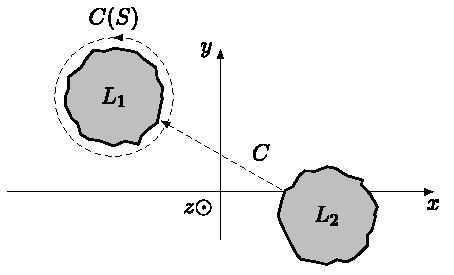
\includegraphics{res/LT1}
\end{center}
%Es soll zudem die \textbf{Dünndrahtnäherung} angesetzt werden, was bedeutet, dass die Stromdichte konstant über den gesamten Leiterquerschnitt ist. Folglich wird der Skin-Effekt ($\nearrow$\ref{skin}) vernachlässigt (das macht man in der Leitungstheorie immer so). Außerdem wird zunächst ein idealer Leiter angesetzt, d.h. es gilt $\kappa\to\infty$. 
Damit folgt
\begin{equation}
	\int\limits_{C}\left(\frac{\partial \vec{\ubar{E}}}{\partial z}+\mathrm{j} \omega \mu \vec{\ubar{H}} \times \vec{e}_{z}\right) \mathrm{d} \vec{r}=\frac{\partial}{\partial z} \underbrace{\int\limits_{C} \vec{\ubar{E}} \mathrm{~d} \vec{r}}_{=\ubar{U}}+\mathrm{j} \omega \mu \int\limits_{C}\left(\vec{\ubar{H}} \times \vec{e}_{z}\right) \mathrm{d} \vec{r}\stackrel{\text{\ref{indang}}}{=}0 
\end{equation}
wobei das magnetische Feld gemäß der Bestimmungsgleichung ($\nearrow$\ref{bestH}) ersetzt und damit die Relation
\begin{equation}
\begin{split}
	\frac{\partial \ubar{U}}{\partial z}+\mathrm{j} \omega \mu \int\limits_{C}\left[\frac{1}{\mathrm{j} \omega \mu} (\vec{e}_{z} \times \grad \ubar{\phi}(x, y))  \frac{\partial \ubar{g}(z)}{\partial z}\right] \times \vec{e}_{z} \mathrm{~d} \vec{r}&=0 \\
	\frac{\partial \ubar{U}}{\partial z}+\frac{\partial \ubar{g}(z)}{\partial z} \int\limits_{C} \grad \ubar{\phi}(x, y) \mathrm{d} \vec{r}&=0 
\end{split}
\end{equation}
erhalten wird. Die partielle Ableitung der Funktion $\ubar{g}(z)$ kann hierfür ohne Weiteres vor das Integral gezogen werden, da die Integration in der $x y$-Ebene erfolgt. ${\partial \ubar{g}(z)}/{\partial z}$ bestimmt man nun in einem nächsten Schritt durch Anwendung des Durchflutungsgesetzes ($\nearrow$\ref{durchf}). Aus der Integration auf dem geschlossenen Weg $C(S)$ entlang der Oberfläche bzw. Berandung eines Leiters folgt der in den Leitern fließende Strom $\ubar{I}$ (in quasistatischer Näherung) gemäß
\begin{equation}\label{fliesstromLT}
	\ubar{I}=\oint\limits_{C(S)} \vec{\ubar{H}} \mathrm{~d} \vec{r}=\frac{1}{\mathrm{j} \omega \mu} \oint\limits_{C(S)}\left(\vec{e}_{z} \times \grad \ubar{\phi}\right) \frac{\partial \ubar{g}(z)}{\partial z} \mathrm{d} \vec{r}=\frac{\partial \ubar{g}(z)}{\partial z} \frac{1}{\mathrm{j} \omega \mu} \oint\limits_{C(S)}\left(\vec{e}_{z} \times \grad \ubar{\phi}\right) \mathrm{d} \vec{r} 
\end{equation}
mit dem sich nach Umstellen die Beziehung
\begin{equation}
	\frac{\partial \ubar{g}(z)}{\partial z}=\frac{\mathrm{j} \omega \mu}{\oint\limits_{C(S)}\left(\vec{e}_{z} \times \grad \ubar{\phi}\right) \mathrm{d} \vec{r}} \cdot \ubar{I} 
\end{equation}
ergibt. Einsetzen in Gleichung \ref{fliesstromLT} führt schließlich auf die \textbf{erste Telegraphengleichung}
\begin{equation}\label{ersttel}
	\frac{\partial \ubar{U}}{\partial z}+\mathrm{j} \omega \underbrace{\mu\frac{\int\limits_{C} \grad \ubar{\phi} \mathrm{d} \vec{r}}{\oint\limits_{C(S)}\left(\vec{e}_{z} \times \grad \ubar{\phi}\right) \mathrm{d} \vec{r}}}_{=: L^{\prime}} \ubar{I}=\boxed{\frac{\partial \ubar{U}}{\partial z}+\mathrm{j} \omega L^{\prime} \ubar{I}=0 }
\end{equation}
Darin wird $L^{\prime}$ als der Induktivitätsbelag der Leitung mit
\begin{equation}\label{indbelag}
	\boxed{L^{\prime}:=\mu \frac{\int\limits_{C} \grad \ubar{\phi}(x, y) \mathrm{d} \vec{r}}{\oint\limits_{C(S)}\left(\vec{e}_{z} \times \grad \ubar{\phi}(x, y)\right) \mathrm{d} \vec{r}} }
\end{equation}
definiert und in der Einheit Henry pro Meter (H/m) angegeben.
\subsubsection{Zweite Telegraphengleichung}
 Die zweite Telegraphengleichung leitet sich in analoger Weise aus dem Durchflutungsgesetz ab. Es ist
\begin{align}
\oint\limits_{C(S)}\left(\frac{\partial \vec{\ubar{H}}}{\partial z}-\mathrm{j} \omega \varepsilon \vec{\ubar{E}} \times \vec{e}_z\right) \mathrm{d} \vec{r} & =\frac{\partial}{\partial z} \oint\limits_{C(S)} \vec{\ubar{H}} \mathrm{~d} \vec{r}-\mathrm{j} \omega \varepsilon \oint\limits_{C(S)}\left(\vec{\ubar{E}} \times \vec{e}_z\right) \mathrm{d} \vec{r} \\
& =\frac{\partial \ubar{I}}{\partial z}+\mathrm{j} \omega \varepsilon \oint\limits_{C(S)}\left(\ubar{g}(z) \grad \ubar{\phi} \times \vec{e}_z\right) \mathrm{d} \vec{r}\stackrel{\text{\ref{indang}}}{=}0
\end{align}
Die unbekannte Funktion $\ubar{g}(z)$ bestimmt sich hier direkt aus der Definition der Spannung $\ubar{U}$ zwischen den Leitern gemäß der Gleichung
\begin{equation}
	\ubar{U}=\int\limits_{C} \vec{\ubar{E}} \mathrm{~d} \vec{r}=-\ubar{g}(z) \int_{C} \grad \ubar{\phi} \mathrm{d} \vec{r} \quad \Rightarrow \quad \ubar{g}(z)=-\frac{\ubar{U}}{\int\limits_{C} \grad \ubar{\phi} \mathrm{d} \vec{r}} 
\end{equation}
sodass man nach Einsetzen die \textbf{zweite Telegraphengleichung} zu
\begin{equation}\label{zweittel}
	\frac{\partial \ubar{I}}{\partial z}+\mathrm{j} \omega \underbrace{\varepsilon\frac{\oint\limits_{C(S)}\left(\vec{e}_z \times\grad \ubar{\phi}\right) \mathrm{d} \vec{r}}{\int\limits_C\grad \ubar{\phi} \mathrm{d} \vec{r}}}_{=: C^{\prime}} \ubar{U}=\boxed{\frac{\partial \ubar{I}}{\partial z}+\mathrm{j} \omega C^{\prime} \ubar{U}=0} \end{equation}

mit der Größe $C^{\prime}$ als dem Kapazitätsbelag der Leitung erhält. Dieser ist über
\begin{equation}\label{kapbelag}
	\boxed{C^{\prime}:=\varepsilon \frac{\oint\limits_{C(S)}\left(\vec{e}_{z} \times \grad \ubar{\phi}\right) \mathrm{d} \vec{r}}{\int\limits_{C} \grad \ubar{\phi} \mathrm{d} \vec{r}}} 
\end{equation}
definiert und wird in der Einheit Farad pro Meter (F/m) angegeben. 
\subsubsection{Interpretation und Entkopplung der Telegraphengleichungen}
Aus den Formeln \ref{indbelag} und \ref{kapbelag} für den Induktivitäts- bzw. Kapazitätsbelag ist ersichtlich, dass die Größen $C^\prime$ und $L^\prime$ vollständig durch die Lösung des statischen 2D-Randwertproblems für $\ubar{\phi}$ im Lösungsvolumen $V$ definiert sind. Das bedeutet, dass man um diese Größen auszurechnen $\Delta \ubar{\phi}=0$ mit $\ubar{\phi}=0$ auf einem Leiter und $\ubar{\phi}=\ubar{U}(z)$ auf dem anderen Leiter lösen muss. % PLENUM: Warum nicht problematisch, wenn man U kennen muss?
Offensichtlich gilt:
\begin{equation}
	L^\prime C^\prime =\varepsilon\mu=\frac{1}{v_\mathrm{c}^2}\quad \implies \quad \boxed{v_\mathrm{c}=\frac{1}{\sqrt{L^\prime C^\prime}}}
\end{equation}
Außerdem kann man die Gleichungen entkoppeln:
	\begin{equation}\label{entkoptel}\begin{split}
	\frac{\partial^2  \ubar{U}(z)}{\partial z^2} + \omega^2 L^\prime C^\prime  \ubar{U}(z) &= 0 \\
	 \frac{\partial^2  \ubar{I}(z)}{\partial z^2} + \omega^2 L^\prime C^\prime  \ubar{I}(z) &= 0
\end{split}\end{equation}
Die Lösungen sind (natürlich) vor- und zurücklaufende Wellen (als ruhende Zeiger):
\begin{equation}\begin{split}
	\ubar{U}(z) &=  \ubar{U}_0  \mathrm{e}^{\pm\mathrm{j}kz} \\
	  \ubar{I}(z)& =  \ubar{I}_0  \mathrm{e}^{\pm\mathrm{j}kz}
	\end{split}\end{equation}
Die Gesamtlösung ist wieder eine Überlagerung aus hin- und rücklaufenden Wellen.
\subsubsection{Matrixschreibweise}
Kompakter können die Gleichungen \ref{ersttel} und \ref{zweittel} in der Matrixform

\begin{equation} \label{matrixformgl}
	\frac{\partial}{\partial z}\binom{\ubar{U}}{\ubar{I}}+\mathrm{j} \omega\left(\begin{array}{cc}
		0 & L^{\prime}  \\
		C^{\prime} & 0
	\end{array}\right)\binom{\ubar{U}}{\ubar{I}}=\binom{0}{0}
\end{equation}
notiert werden.
\subsection{Konstruktion des Leitungsersatzschaltbildes}
\subsubsection{Verlustloser Fall}
Auf Grundlage der Telegraphengleichungen ist ein Übergang zu folgendem Leitungsersatzschaltbild möglich
\begin{center}
	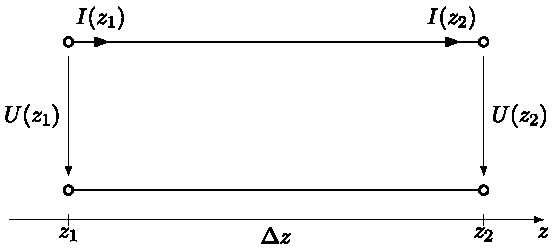
\includegraphics{res/LT2}
\end{center}
Zu einer Lösung des Differentialgleichungssystems gelangt man durch Entkoppeln beider Gleichungen, indem eine von ihnen erneut nach $z$ abgeleitet und anschließend die jeweils andere Gleichung darin eingesetzt wird. Das wird in Gleichung \ref{entkoptel} angedeutet. Für Differentialgleichungssysteme der Form
\begin{equation}
	\frac{\mathrm{d} \vec{y}(x)}{\mathrm{d} x}+\mathbf{A} \vec{y}(x)=\vec{0} 
\end{equation}
mit konstanter Koeffizientenmatrix $\mathbf{A}$ ist eine formale Lösung allerdings auch über den Exponentialansatz
\begin{equation}
	\vec{y}(x)=\vec{C} \mathrm{e}^{-\mathbf{A} x}
\end{equation}
möglich. Der Konstantenvektor $\vec{C} \in \mathbb{C}^{n}$ bestimmt sich dann aus einem Randwert $x_{0}$ und man erhält
\begin{equation}
	\begin{array}{rlrl}
		\vec{y}\left(x_{0}\right) & =\vec{C} \mathrm{e}^{-\mathbf{A} x_{0}} \quad \rightarrow \quad \vec{C}=\mathrm{e}^{\mathbf{A} x_{0}} \vec{y}\left(x_{0}\right) \\
		\vec{y}(x) & =\mathrm{e}^{-\mathbf{A}\left(x-x_{0}\right)} \vec{y}\left(x_{0}\right) & 
	\end{array}
\end{equation}
Für das konkrete Differentialgleichungssystem \ref{matrixformgl} folgt also mit den Randwerten am Leitungsabschluss
\begin{equation}
	\binom{\ubar{U}(z)}{\ubar{I}(z)}=\mathrm{e}^{-\mathbf{A}\left(z-z_{2}\right)}\binom{\ubar{U}\left(z_{2}\right)}{\ubar{I}\left(z_{2}\right)}=\mathrm{e}^{\mathbf{A}\left(z_{2}-z\right)}\binom{\ubar{U}\left(z_{2}\right)}{\ubar{I}\left(z_{2}\right)} 
\end{equation}
Am Anfang des Leiterstückes an der Stelle $z_{1}$ gilt dann mit der Leitungslänge $\Delta z=z_{2}-z_{1}$
\begin{equation}
\binom{\ubar{U}\left(z_{1}\right)}{\ubar{I}\left(z_{1}\right)}=\mathrm{e}^{\mathbf{A} \Delta z}\binom{\ubar{U}\left(z_{2}\right)}{\ubar{I}\left(z_{2}\right)} \quad \text { mit } \quad \mathbf{A}=\mathrm{j} \omega\left(\begin{array}{cc}
	0 & L^{\prime}  \\
	C^{\prime} & 0
\end{array}\right)
\end{equation}
Für eine hinreichend kleine Leiterlänge $\Delta z$ lässt sich der Matrixexponent dann über
\begin{equation}
	\mathrm{e}^{\mathbf{A} \Delta z}=\mathbf{E}+\mathbf{A} \Delta z+\frac{1}{2} \mathbf{A}^{2}(\Delta z)^{2}+\frac{1}{3} \mathbf{A}^{3}(\Delta z)^{3}+\ldots 
\end{equation}
in eine Reihe entwickeln, wobei nach dem linearen Term abgebrochen werden kann. Somit folgt
\begin{equation}\begin{split}
\binom{\ubar{U}\left(z_{1}\right)}{\ubar{I}\left(z_{1}\right)}=\left[\left(\begin{array}{ll}
	1 & 0  \\
	0 & 1
\end{array}\right)+\mathrm{j} \omega\left(\begin{array}{cc}
	0 & L^{\prime} \\
	C^{\prime} & 0
\end{array}\right) \Delta z\right]\binom{\ubar{U}\left(z_{2}\right)}{\ubar{I}\left(z_{2}\right)}&\\
=\left(\begin{array}{cc}
	1 & \mathrm{j} \omega L^{\prime} \Delta z \\
	\mathrm{j} \omega C^{\prime} \Delta z & 1
\end{array}\right)\binom{\ubar{U}\left(z_{2}\right)}{\ubar{I}\left(z_{2}\right)}
\end{split}\end{equation}
Als nächster Schritt ist zur Bestimmung eines Ersatzschaltbildes der Leitung ein Vierpol in $A$-Parameterdarstellung bzw. Kettenmatrixform mit
\begin{equation}
\binom{\ubar{U}_{1}}{\ubar{I}_{1}}=\left(\begin{array}{ll}
	A_{11} & A_{12}  \\
	A_{21} & A_{22}
\end{array}\right)\binom{\ubar{U}_{2}}{\ubar{I}_{2}}
\end{equation}
gesucht. Welcher Vierpol besitzt also die zuvor bestimmten $A$-Parameter? Man betrachte dazu das in folgender Abbildung dargestellte Zweitor mit der Reiheninduktivität $L^{\prime} \Delta z$ und der Parallelkapazität $C^{\prime} \Delta z$.
\begin{center}
	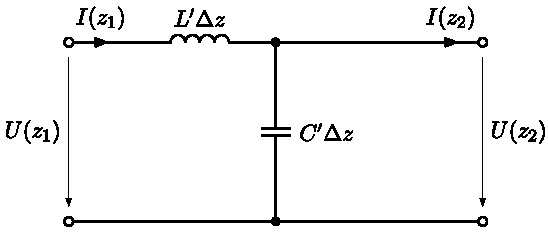
\includegraphics{res/LT3}
\end{center}
Dessen Parametermatrix stellt sich folgendermaßen dar
\begin{equation}
\left(\begin{array}{cc}
	1 & \mathrm{j} \omega L^{\prime} \Delta z  \\
	0 & 1
\end{array}\right)\left(\begin{array}{cc}
	1 & 0 \\
	\mathrm{j} \omega C^{\prime} \Delta z & 1
\end{array}\right)=\left(\begin{array}{cc}
	1-\omega^{2} L^{\prime} C^{\prime} \Delta z^{2} & \mathrm{j} \omega L^{\prime} \Delta z \\
	\mathrm{j} \omega C^{\prime} \Delta z & 1
\end{array}\right)
\end{equation}
Bis auf den additiven Term $\omega^{2} L^{\prime} C^{\prime}(\Delta z)^{2}$ stimmt diese Darstellung mit dem vorigen Ergebnis überein. Das bedeutet, für den Fall $\omega^{2} L^{\prime} C^{\prime}(\Delta z)^{2} \ll 1$ ist das verwendete Ersatzschaltbild gültig. Anders ausgedrückt heißt dies
\begin{equation}
	(\Delta z)^{2} \ll \frac{1}{\omega^{2} L^{\prime} C^{\prime}} \stackrel{L^{\prime} C^{\prime}=\frac{1}{v_\mathrm{c}^{2}}}{=} \frac{v_\mathrm{c}^{2}}{\omega^{2}} \stackrel{k=\frac{\omega}{v_\mathrm{c}}}{=} \frac{1}{k^{2}} \stackrel{k=\frac{2 \pi}{\lambda}}{=} \frac{\lambda^{2}}{(2 \pi)^{2}} 
\end{equation}
Als Bedingung für die Wellenlänge der sich auf der Leitung ausbreitenden Welle leitet sich hieraus das sogenannte $\lambda / 10-$ Kriterium
\begin{equation}
	\lambda \gg 2 \pi \Delta z \approx 6 \Delta z \approx 10 \Delta z 
\end{equation}
ab. Ist dieses erfüllt, kann obiges Ersatzschaltbild als Leitungsmodell herangezogen werden. Im Grenzfall $\Delta z \to 0$ ist das Ersatzschaltbild sogar exakt. Das kann beispielsweise gezeigt werden, indem für das obige Ersatzschaltbild Maschen- und Knotensatz aufgestellt werden:
\begin{itemize}
	\item  Maschensatz:
	\begin{equation}\begin{split}
			\ubar{U}(z_1) = \mathrm{j}\omega \underbrace{L}_{L'\Delta z}  \ubar{I}(z_1) +  \ubar{U}(\underbrace{z_1+\Delta z}_{z_2})\\
			\ubar{U}(z_1+\Delta z) - \ubar{U}(z_1) + \mathrm{j}\omega L  \ubar{I}(z_1) =0  \\
			\frac{\Delta  \ubar{U}}{\Delta z} + \mathrm{j}\omega \frac{L}{\Delta z}  \ubar{I}(z_1) =0
	\end{split}\end{equation}
	
	\item Knotensatz:
	\begin{equation}
		\ubar{I}(z_1+\Delta z) =  \ubar{I}(z_1) - \mathrm{j}\omega \underbrace{C}_{C'\Delta z}  \ubar{U}(z_1+\Delta z) \Rightarrow \frac{\Delta  \ubar{I}}{\Delta z} + \mathrm{j}\omega \frac{C}{\Delta z}  \ubar{U}(z_1+\Delta z) = 0
	\end{equation}
\end{itemize}
Im Grenzübergang $\Delta z \to 0$ entsprechen diese Gleichungen exakt den Telegraphengleichungen \ref{ersttel} und \ref{zweittel}, weshalb der Vierpol das Ersatzschaltbild für ein verlustloses Stück Leitung (für das gelten die Telegraphengleichungen) sein muss.
\subsubsection{Verallgemeinerung zum verlustbehafteten Fall}
Anhand der gefundenen Vierpoldarstellung konnte nun gezeigt werden, dass ein \textbf{Leitungsmodell} mit \textbf{Längsinduktivität} und \textbf{Querkapazität} ein gültiges \textbf{Ersatzschaltbild} des \textbf{differentiellen Leiterstückes} darstellt. Hieraus lässt sich auch ein um die \textbf{Leitungsverluste} \textbf{erweitertes Modell} ableiten, mithilfe dessen eine entkoppelte Lösung für Spannung $\ubar{U}(z)$ und Strom $\ubar{I}(z)$ entlang der Leitung bestimmt werden kann. Dafür werden Spule und Kondensator durch ihre verlustbehafteten Äquivalente substituiert. Für ein Segment der Länge $\Delta z$ stellt sich das Ersatzschaltbild für eine verlustbehaftete Leitung also wie in folgender Grafik dar:
\begin{center}
	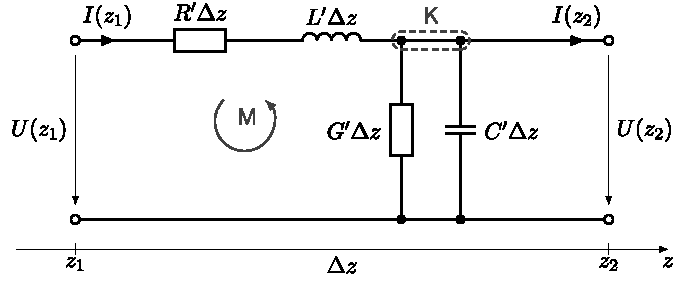
\includegraphics{res/LT4}
\end{center}
Der \textbf{Widerstandsbelag} $R'$ entspricht den ohmschen Leitungsverlusten pro Längeneinheit, der \textbf{Leitwertbelag} $G'$ entspricht den dielektrischen Verlusten. Zusammengefasst spricht man auch von \textbf{Impdeanzbelag} $R^{\prime}+\mathrm{j} \omega L^{\prime}$ und \textbf{Admittanzbelag} $G^{\prime}+\mathrm{j} \omega C^{\prime}$. Anwendung von Maschen- und Knotensatz liefert
\begin{align}
	&& M: \quad \ubar{U}(z)&=\ubar{U}(z+\Delta z)+\left(R^{\prime} \Delta z\right) \ubar{I}(z)+\mathrm{j} \omega\left(L^{\prime} \Delta z\right) \ubar{I}(z)  \\
	&& K: \quad \ubar{I}(z)&=\ubar{I}(z+\Delta z)+\ubar{U}(z+\Delta z)\left(G^{\prime} \Delta z\right)+\mathrm{j} \omega\left(C^{\prime} \Delta z\right) \ubar{U}(z+\Delta z) 
\end{align}
\subsubsection{Differentialgleichungssystem für den verlustbehafteten Fall}
Nach Übergang vom Differenzenquotienten zum Differentialquotienten mit $\Delta z \rightarrow 0$ erhält man
\begin{equation}
\frac{\mathrm{d}}{\mathrm{d} z}\binom{\ubar{U}(z)}{\ubar{I}(z)}+\left(\begin{array}{cc}
	0 & R^{\prime}+\mathrm{j} \omega L^{\prime}  \\
	G^{\prime}+\mathrm{j} \omega C^{\prime} & 0
\end{array}\right)\binom{\ubar{U}(z)}{\ubar{I}(z)}=\binom{0}{0}
\end{equation}
Die Entkopplung dieses Differentialgleichungssystems führt auf die DGL zweiter Ordnung
\begin{equation}\begin{split}
	\frac{\mathrm{d}^{2}}{\mathrm{~d} z^{2}} \ubar{U}(z)&=-\left(R^{\prime}+\mathrm{j} \omega L^{\prime}\right) \frac{\mathrm{d} \ubar{I}(z)}{\mathrm{d} z}=\underbrace{\left(R^{\prime}+\mathrm{j} \omega L^{\prime}\right)\left(G^{\prime}+\mathrm{j} \omega C^{\prime}\right)}_{=: \ubar{\gamma}^{2}} \ubar{U}(z)\\
	\Aboxed{\ubar{\gamma}&=\sqrt{\left(R^{\prime}+\mathrm{j} \omega L^{\prime}\right)\left(G^{\prime}+\mathrm{j} \omega C^{\prime}\right)}}
\end{split}\end{equation}
deren Lösung man zu
\begin{equation} \label{loesULT}
	\boxed{\ubar{U}(z)=\ubar{U}^{+} \mathrm{e}^{-\ubar{\gamma} z}+\ubar{U}^{-} \mathrm{e}^{+\ubar{\gamma} z} }
\end{equation}
bestimmt. Diese stellt im Grunde eine Überlagerung der in positiver (erster Summand) und negativer $z$-Richtung (zweiter Summand) propagierenden Welle dar. Die additive (anstelle einer subtraktiven) Überlagerung ist Konvention. Für den Strom $\ubar{I}(z)$ gilt dann
\begin{align}
	\ubar{I}(z) & =-\frac{1}{R^{\prime}+\mathrm{j} \omega L^{\prime}} \frac{\mathrm{d} \ubar{U}(z)}{\mathrm{d} z}=\frac{\ubar{\gamma}}{R^{\prime}+\mathrm{j} \omega L^{\prime}}\left(\ubar{U}^{+} \mathrm{e}^{-\ubar{\gamma} z}-\ubar{U}^{-} \mathrm{e}^{+\ubar{\gamma} z}\right)  \\
	& =\underbrace{\sqrt{\frac{G^{\prime}+\mathrm{j} \omega C^{\prime}}{R^{\prime}+\mathrm{j} \omega L^{\prime}}}}_{=: \frac{1}{\ubar{Z}_{\mathrm{C}}}}\left(\ubar{U}^{+} \mathrm{e}^{-\ubar{\gamma} z}-\ubar{U}^{-} \mathrm{e}^{+\ubar{\gamma} z}\right)=\boxed{\frac{1}{\ubar{Z}_{\mathrm{C}}}\left(\ubar{U}^{+} \mathrm{e}^{-\ubar{\gamma} z}-\ubar{U}^{-} \mathrm{e}^{+\ubar{\gamma} z}\right)=\ubar{I}(z)} \label{loesILT}
\end{align}
Hierin ist die Größe
\begin{equation}
	\boxed{\ubar{Z}_{\mathrm{C}}=\sqrt{\frac{R^{\prime}+\mathrm{j} \omega L^{\prime}}{G^{\prime}+\mathrm{j} \omega C^{\prime}}} }
\end{equation}
die sogenannte \textbf{charakteristische Impedanz} bzw. \textbf{Leitungswellenwiderstand} der Leitung. Es ist zu beachten, dass dieser nicht gleich dem Feldwellenwiderstand ist. Weiterhin nennt man $R^{\prime}, G^{\prime}, L^{\prime}$ und $C^{\prime}$ die \textbf{primären Leitungsparameter}, während man $\ubar{\gamma}$ und $\ubar{Z}_{\mathrm{C}}$ als \textbf{sekundäre Leitungsparameter} bezeichnet.
Die noch unbekannten Integrationskonstanten $\ubar{U}^{+}$und $\ubar{U}^{-}$lassen sich aus den Anfangswerten von Spannung und Strom am Leitungseingang ermitteln. Für $z=0$ ist
\begin{equation}
	\ubar{U}(0)=\ubar{U}^{+}+\ubar{U}^{-} \quad \text { und } \quad \ubar{I}(0)=\frac{1}{\ubar{Z}_{\mathrm{C}}}\left(\ubar{U}^{+}-\ubar{U}^{-}\right)
\end{equation}
Hiermit bestimmen sich die Konstanten zu
\begin{equation}
	\ubar{U}^{+}=\frac{1}{2}\left[\ubar{U}(0)+\ubar{Z}_{\mathrm{C}} I(0)\right] \quad \text { bzw. } \quad \ubar{U}^{-}=\frac{1}{2}\left[\ubar{U}(0)-\ubar{Z}_{\mathrm{C}} \ubar{I}(0)\right] 
\end{equation}
Einsetzen in \ref{loesULT} und anschließende Umformung liefert
\begin{align}
	\ubar{U}(z) & =\ubar{U}^{+} \mathrm{e}^{-\ubar{\gamma} z}+\ubar{U}^{-} \mathrm{e}^{+\ubar{\gamma} z}=\frac{1}{2}\left[\ubar{U}(0)+\ubar{Z}_{\mathrm{C}} \ubar{I}(0)\right] \mathrm{e}^{-\ubar{\gamma} z}+\frac{1}{2}\left[\ubar{U}(0)-\ubar{Z}_{\mathrm{C}} \ubar{I}(0)\right] \mathrm{e}^{+\ubar{\gamma} z}  \\
	\Aboxed{\ubar{U}(z)& =\ubar{U}(0) \cosh (\ubar{\gamma} z)-\ubar{Z}_{\mathrm{C}} \ubar{I}(0) \sinh (\ubar{\gamma} z) }
\end{align}
Gleichfalls folgt für den Strom
\begin{equation}
	\boxed{\ubar{I}(z)=-\frac{1}{\ubar{Z}_{\mathrm{C}}} \ubar{U}(0) \sinh (\ubar{\gamma} z)+\ubar{I}(0) \cosh (\ubar{\gamma} z)}
\end{equation}
Die vollständige Leitung wird somit durch einen Vierpol mit der Matrixform

\begin{equation}
\binom{\ubar{U}(z)}{\ubar{I}(z)}=\left(\begin{array}{cc}
	\cosh (\ubar{\gamma} z) & -\ubar{Z}_{\mathrm{C}} \sinh (\ubar{\gamma} z)  \\
	-\frac{1}{\ubar{Z}_{\mathrm{C}}} \sinh (\ubar{\gamma} z) & \cosh (\ubar{\gamma} z)
\end{array}\right)\binom{\ubar{U}(0)}{\ubar{I}(0)}
\end{equation}
beschrieben. 
\subsubsection{Impedanztransformation entlang einer Leitung}
Stellt man diese Gleichung nun um und wertet das Ganze bei $z=L$ aus, dann erhält man 
\begin{equation}
\binom{\ubar{U}(0)}{\ubar{I}(0)}=\left(\begin{array}{cc}
	\cosh (\ubar{\gamma} L) & Z_{\mathrm{C}} \sinh (\ubar{\gamma} L)  \\
	\frac{1}{Z_{\mathrm{C}}} \sinh (\ubar{\gamma} L) & \cosh (\ubar{\gamma} L)
\end{array}\right)\binom{\ubar{U}(L)}{\ubar{I}(L)}
\end{equation}
Damit könnte man nun ${\ubar{U}(0)}/{\ubar{I}(0)}$ bilden und würde die Eingangsimpedanz bei $z=0$ erhalten, die bei einer gewissen Ausgangsimpedanz ${\ubar{U}(L)}/{\ubar{I}(L)}$ zu sehen ist. Das lässt sich verallgemeinern, sodass man die Eingangsimpedanz bei einem beliebigen $z$ berechnen kann, wenn am Ausgang bei $z=L$ die Ausgangsimpedanz ${\ubar{U}(L)}/{\ubar{I}(L)}$ zu sehen ist. Dafür ist eine Auswertung bei $z$ anstatt bei $0$ erforderlich. Der Abstand von $z$ zu $L$ (also die transformierende Leitungslänge) ist dann $L-z$ anstelle von $L$. Mit
\begin{equation}
	\frac{\ubar{U}(z)}{\ubar{I}(z)}=\frac{\cosh (\ubar{\gamma}(L-z)) \ubar{U}(L)+\ubar{Z}_{\mathrm{C}} \sinh (\ubar{\gamma}(L-z)) \ubar{I}(L)}{\frac{1}{\ubar{Z}_{\mathrm{C}}} \sinh (\ubar{\gamma}(L-z)) \ubar{U}(L)+\cosh (\ubar{\gamma}(L-z)) \ubar{I}(L)} 
\end{equation}
lässt sich nun die Eingangsimpedanz an der Stelle $z$ berechnen. Weitere Umformung durch teilen des Zählers und Nenners durch $\ubar{I}(L)\cosh (\ubar{\gamma}(L-z))$ liefert schließlich
\begin{align}
	 \frac{\ubar{U}(z)}{\ubar{I}(z)}&=\frac{\frac{\ubar{U}(L)}{\ubar{I}(L)}+\ubar{Z}_{\mathrm{C}} \tanh (\ubar{\gamma}(L-z))}{\frac{1}{\ubar{Z}_{\mathrm{C}}} \frac{\ubar{U}(L)}{\ubar{I}(L)} \tanh (\ubar{\gamma}(L-z))+1}=\frac{\ubar{Z}_{\mathrm{a}}+\ubar{Z}_{\mathrm{C}} \tanh (\ubar{\gamma}(L-z))}{1+\frac{\ubar{Z}_{\mathrm{a}}}{\ubar{Z}_{\mathrm{C}}} \tanh (\ubar{\gamma}(L-z))}  \\
	\Aboxed{\ubar{Z}(z)&=Z_{\mathrm{a}} \frac{1+\frac{\ubar{Z}_{\mathrm{C}}}{\ubar{Z}_{\mathrm{a}}} \tanh (\ubar{\gamma}(L-z))}{1+\frac{\ubar{Z}_{\mathrm{a}}}{\ubar{Z}_{\mathrm{C}}} \tanh (\ubar{\gamma}(L-z))}}
\end{align}
mit der Last- bzw. Abschlussimpedanz $\ubar{Z}_{\mathrm{a}}=\frac{\ubar{U}(L)}{\ubar{I}(L)}$. 
\subsubsection{Reflektionsfaktor}
Der Reflexionsfaktor $\ubar{\Gamma}(z)$ der Leitung an der Stelle $z$ ist nun definiert als das Verhältnis von rücklaufender zu hinlaufender Welle mit
\begin{align}
	\ubar{U}(z) & =\ubar{U}^{+} \mathrm{e}^{-\ubar{\gamma} z}+\ubar{U}^{-} \mathrm{e}^{+\ubar{\gamma} z}=\ubar{U}^{+} \mathrm{e}^{-\ubar{\gamma} z}\left(1+\frac{\ubar{U}^{-}}{\ubar{U}^{+}} \mathrm{e}^{2 \ubar{\gamma} z}\right)  \\
	& =\ubar{U}^{+} \mathrm{e}^{-\ubar{\gamma} z}(1+\ubar{\Gamma}(z)) \quad \text { mit } \quad \boxed{\ubar{\Gamma}(z):=\frac{\ubar{U}^{-}}{\ubar{U}^{+}} \mathrm{e}^{2 \ubar{\gamma} z} }
\end{align}
Für die Eingangsimpedanz schreibt sich damit
\begin{equation}
	\ubar{Z}(z)=\frac{\ubar{U}(z)}{\ubar{I}(z)}=\frac{\ubar{U}^{+} \mathrm{e}^{-\ubar{\gamma} z}+\ubar{U}^{-} \mathrm{e}^{+\ubar{\gamma} z}}{\frac{1}{\ubar{Z}_{\mathrm{C}}}\left(\ubar{U}^{+} \mathrm{e}^{-\ubar{\gamma} z}-\ubar{U}^{-} \mathrm{e}^{+\ubar{\gamma} z}\right)}=\ubar{Z}_{\mathrm{C}} \frac{1+\ubar{\Gamma}(z)}{1-\ubar{\Gamma}(z)} 
\end{equation}
Umstellen nach dem Reflexionsfaktor liefert
\begin{equation}
	\boxed{\ubar{\Gamma}(z)=\frac{\ubar{Z}(z)-\ubar{Z}_{\mathrm{C}}}{\ubar{Z}(z)+\ubar{Z}_{\mathrm{C}}}} \quad, \quad \ubar{\Gamma}(L)=\frac{\ubar{Z}(L)-\ubar{Z}_{\mathrm{C}}}{\ubar{Z}(L)+\ubar{Z}_{\mathrm{C}}}=\frac{\ubar{Z}_{\mathrm{a}}-\ubar{Z}_{\mathrm{C}}}{\ubar{Z}_{\mathrm{a}}+\ubar{Z}_{\mathrm{C}}} 
\end{equation}
Eine Impedanz korrespondiert also über eine Möbius-Transformation mit einem Reflektionsfaktor. Es ist also möglich das Verhältnis der einlaufenden zur reflektierten Welle vorherzusagen, ohne die Wellen explizit zu berechnen.
\subsubsection{Beispiel (Dämpfungsferrite auf Leitungen)}
Zur Unterdrückung von Gleichtaktstörungen auf Versorgungs- oder Datenleitungen werden in der Praxis Dämpfungsferrite eingesetzt. Zur konkreten Auslegung ist eine analytische Beschreibung der Leitung mit Ferrit notwendig. Intuitiv würde man zunächst folgendes Modell mit einer frequenzabhängigen Ferritimpedanz $Z_{\mathrm{Fe}}$ annehmen:
\begin{center}
	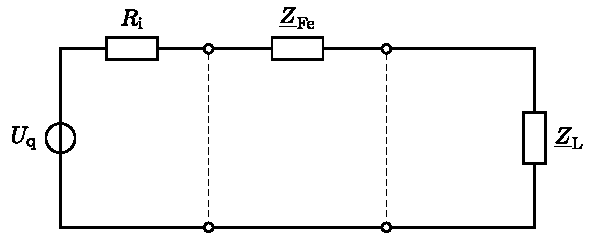
\includegraphics{res/LT51}
\end{center}
Diese Vorstellung stellt sich jedoch als physikalisch falsch heraus, da bei offenem Abschluss mit $\ubar{Z}_{\mathrm{e}} \rightarrow \infty$ kein Strom fließen dürfte. Durch einfache Messungen mit einem Netzwerkanalysator kann allerdings gezeigt werden, dass aufgrund der Leitungskapazität stets ein gewisser Verschiebungsstrom feststellbar ist. Man darf also nicht ohne Weiteres verteilte Leitungsparameter mit konzentrierten elektrischen Elementen kombinieren.
Als alternatives Beschreibungsmittel bietet sich hingegen die Leitungstheorie an. Dazu werde der nachfolgend dargestellte Versuchsaufbau betrachtet.
\begin{center}
	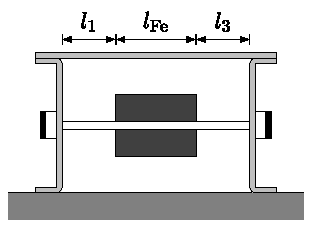
\includegraphics{res/LT52}
\end{center}
Mithilfe eines Netzwerkanalysators werden die $S$-Parameter der Leitung bei Einspeisung an Port 2 und Messung an Port 1 bestimmt, wobei der Übertragungsfaktor $\ubar{S}_{21}$ die interessierende Größe darstellt. Zur rechnerischen Bestimmung von $\ubar{S}_{21}$ und der Eingangsimpedanz $\ubar{Z}_{\mathrm{e}}$ müssen die drei Leitungsabschnitte $z \in[0 ; L],\left[L_{1} ; L_{2}\right]$ und $\left[L_{2} ; L\right]$ zusammengefasst werden, wofür die Nutzung von Ketternparametern sinnvoll ist.
\subsection{Mehrfachleitungen}
Unter einer Mehrfachleitung versteht man eine Gruppe von $n$ Leitern zuzüglich eines Referenzleiters (siehe nachfolgende Grafik). Zur Bestimmung der Spannungen und Ströme innerhalb einer solchen Anordnung müssen die Leitungsgleichungen entsprechend erweitert werden.
\begin{center}
	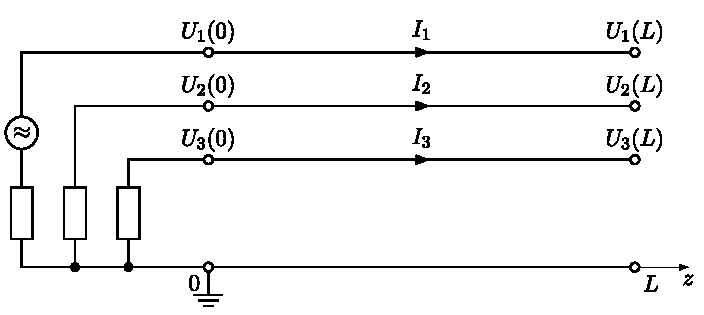
\includegraphics{res/LT7}
\end{center}
Für ein allgemeines $n$-Leitersystem formulieren sich die Telegraphengleichungen \ref{ersttel} und \ref{zweittel} (bzw. in Matrixform: \ref{matrixformgl}) in der verallgemeinerten Matrixform
\begin{equation}\label{verallgmatr}\begin{split}
	\frac{\mathrm{d}}{\mathrm{d} z}\left(\begin{array}{c}
		\ubar{U}_{1}  \\
		\ubar{U}_{2} \\
		\vdots \\
		\ubar{U}_{n}
	\end{array}\right)+\ubar{\mathbf{Z}}^{\prime}\left(\begin{array}{c}
		\ubar{I}_{1} \\
		\ubar{I}_{2} \\
		\vdots \\
		\ubar{I}_{n}
	\end{array}\right)&=\left(\begin{array}{c}
		0 \\
		0 \\
		\vdots \\
		0
	\end{array}\right) \\ \frac{\mathrm{d}}{\mathrm{d} z}\left(\begin{array}{c}
		\ubar{I}_{1} \\
		\ubar{I}_{2} \\
		\vdots \\
		\ubar{I}_{n}
	\end{array}\right)+\ubar{\mathbf{Y}}^{\prime}\left(\begin{array}{c}
		\ubar{U}_{1} \\
		\ubar{U}_{2} \\
		\vdots \\
		\ubar{U}_{n}
	\end{array}\right)&=\left(\begin{array}{c}
		0 \\
		0 \\
		\vdots \\
		0
	\end{array}\right)
\end{split}\end{equation}

mit den $n$-Spaltenvektoren $\vec{\ubar{U}}$ und $\vec{\ubar{I}}$ der Leiterspannungen bzw. Leiterströme. Zudem bezeichnen darin $\ubar{\mathbf{Z}}^{\prime}=\mathbf{R}^{\prime}+\mathrm{j} \omega \mathbf{L}^{\prime}$ die $n \times n$ Impedanzmatrix und $\ubar{\mathbf{Y}}^{\prime}=\mathbf{G}^{\prime}+\mathrm{j} \omega \mathbf{C}^{\prime}$ die $n \times n$ Admittanzmatrix. Sie repräsentieren die Resistivitäten, Konduktivitäten, Induktivitäten und Kapazitäten der Einzelleiter sowie der Leitungen untereinander und bilden somit die wechselseitige Beeinflussung innerhalb des Leitersystems ab. Die Impedanzmatrix besitzt die Gestalt
\begin{equation}
	\ubar{\mathbf{Z}}^{\prime}=\left(\begin{array}{cccc}
		R_{1}^{\prime}+R_{\mathrm{G} 11}^{\prime} & R_{\mathrm{G} 12}^{\prime} & \cdots & R_{\mathrm{G} 1 n}^{\prime}  \\
		R_{\mathrm{G} 21}^{\prime} & R_{2}^{\prime}+R_{\mathrm{G} 22}^{\prime} & \cdots & R_{\mathrm{G} 2 n}^{\prime} \\
		\vdots & \vdots & \ddots & \vdots \\
		R_{\mathrm{G} n 1}^{\prime} & R_{\mathrm{G} n 2}^{\prime} & \cdots & R_{n}^{\prime}+R_{\mathrm{G} n n}^{\prime}
	\end{array}\right)+\mathrm{j} \omega\left(\begin{array}{cccc}
		L_{11}^{\prime} & M_{12}^{\prime} & \cdots & M_{1 n}^{\prime} \\
		M_{21}^{\prime} & L_{22}^{\prime} & \cdots & M_{2 n}^{\prime} \\
		\vdots & \vdots & \ddots & \vdots \\
		M_{n 1}^{\prime} & M_{n 2}^{\prime} & \cdots & L_{n n}^{\prime}
	\end{array}\right)
\end{equation}
und enthält die Widerstandsbeläge $R_{i}^{\prime}$ und Selbstinduktivitätsbeläge $L_{i i}^{\prime}$ eines jeden Einzelleiters $i$ sowie die Widerstandbeläge $R_{\mathrm{G} i j}^{\prime}$ des gemeinsamen Rückleiters und Gegeninduktivitätsbeläge $M_{i j}^{\prime}$ zwischen den Leitern $i$ und $j$. Ähnlich verhält es sich mit der Admittanzmatrix
\begin{equation}
	\ubar{\mathbf{Y}}^{\prime}=\left(\begin{array}{cccc}
		G_{11}^{\prime} & G_{12}^{\prime} & \cdots & G_{1 n}^{\prime}  \\
		G_{21}^{\prime} & G_{22}^{\prime} & \cdots & G_{2 n}^{\prime} \\
		\vdots & \vdots & \ddots & \vdots \\
		G_{n 1}^{\prime} & G_{n 2}^{\prime} & \cdots & G_{n n}^{\prime}
	\end{array}\right)+\mathrm{j} \omega\left(\begin{array}{cccc}
		C_{11}^{\prime} & -C_{12}^{\prime} & \cdots & -C_{1 n}^{\prime} \\
		-C_{21}^{\prime} & C_{22}^{\prime} & \cdots & -C_{2 n}^{\prime} \\
		\vdots & \vdots & \ddots & \vdots \\
		-C_{n 1}^{\prime} & -C_{n 2}^{\prime} & \cdots & C_{n n}^{\prime}
	\end{array}\right)
\end{equation}
deren Elemente aus den Leitwertbelägen $G_{i j}^{\prime}$ und Koppelkapazitätsbelägen $C_{i j}^{\prime}$ zwischen den Leitern $i$ und $j$ gebildet werden.
Obiges Differentialgleichungssystem lässt sich aufgrund der Tatsache, dass die Systemmatrizen jeweils voll besetzt sind, nicht auf herkömmlichem Wege mit einem Exponentialansatz oder einer Variation der Konstanten lösen. Man nutzt hierzu stattdessen die sogenannte \textbf{modale Analyse}.
\section{Allgemeine Leitungstheorie}\label{allgleit}
Im Gegensatz zur klassischen Leitungstheorie, welche Gegenstand des vorigen Abschnitts war und die sich im Wesentlichen auf die Ausbreitung dominierender TEM-Wellenmoden auf homogenen und geradlinigen Leiteranordnungen beschränkt (in den dort betrachteten Fällen sind exakte Beziehungen zwischen Feld- und Leitergrößen angebbar), berücksichtigt die allgemeine Leitungstheorie auch inhomogene Strukturen und ungleichförmige Leitungen inklusive der auftretenden elektromagnetischen Strahlungsphänomene. Im Gegensatz zum vorherigen Abschnitt muss hier genähert werden, dafür sind die betrachteten Anordnungen realistischer (z.B. keine unendlichen Leitungen).\\
Beispielsweise lassen sich die in der folgenden Abbildung dargestellten Leiteranordnungen durch die klassische Theorie nicht mehr exakt beschreiben, da es vor allem an Leiterunstetigkeiten zur Beschleunigung elektrischer Ladungen und infolgedessen zu elektromagnetischer Abstrahlung kommt.\\
\begin{center}
	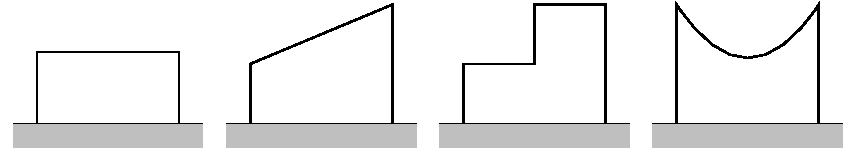
\includegraphics{res/LT15}
\end{center}
Für \textbf{ein Beispiel} soll im Folgenden eine näherungsweise mathematische Beschreibungsweise ähnlich den Telegraphengleichungen gefunden werden.
\subsection{Grundsätzliche Betrachtungen}
Üblicherweise nutzt man im Kontext elektromagnetischer Wellen die Lorenz-Eichung ($\nearrow$\ref{lorenzeich}). Mit der Greenschen Funktion 
\begin{equation}
	\ubar{G}\left(\vec{r}, \vec{r}^{\prime}, k\right)=\frac{\mathrm{e}^{-\mathrm{j} k\left|\vec{r}-\vec{r}^{\prime}\right|}}{|\vec{r}-\vec{r}|} 
\end{equation}
im Freiraum erhält man die partikulären Lösungen ($\nearrow$\ref{skalarpotlor},\ref{vekpotlor})
\begin{align}
	\ubar{\phi}(\vec{r}) & =\frac{1}{4 \pi \varepsilon} \iiint\limits_{V^{\prime}} \ubar{\rho}_{\mathrm{V}}\left(\vec{r}^{\prime}\right) \ubar{G}\left(\vec{r}, \vec{r}^{\prime}, k\right) \mathrm{d} V^{\prime} \label{partLT1}  \\
	\vec{\ubar{A}}(\vec{r}) & =\frac{\mu}{4 \pi} \iiint\limits_{V^{\prime}} \vec{\ubar{J}}\left(\vec{r}^{\prime}\right) \ubar{G}\left(\vec{r}, \vec{r}^{\prime}, k\right) \mathrm{d} V^{\prime}  \label{partLT2}
\end{align}
als die sogenannten retardierten Potentiale, wobei $k=\frac{\omega}{v_\mathrm{c}}=\frac{2 \pi}{\lambda}$ wiederum die Wellenzahl im Medium darstellt. Die betrachtete Übertragungsleitung sei weiterhin als beliebig im Raum entlang der Kurve $C$ verlaufende, \textbf{dünne Drahtstruktur} eines idealen Leiters angenommen, die den Strom $\ubar{I}\left(\vec{r}^{\prime}\right)$ trage (links in folgender Abbildung).
\begin{center}
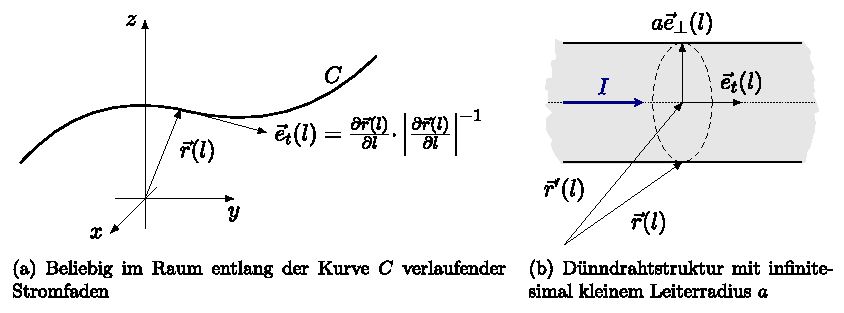
\includegraphics{res/LT16}
\end{center}
Der räumliche Kurvenverlauf wird dabei in krummlinigen Koordinaten durch den Parameter $l \in[0 ; L]$ beschrieben, welcher zwischen Null und der Leiterlänge $L$ variiert. Jene entspricht somit der Bogenlänge der Kurve, die über das Wegintegral
\begin{equation}
	L=\int\limits_{\vec{r}(0)}^{\vec{r}(L)}\left|\frac{\partial \vec{r}(l)}{\partial l}\right| \mathrm{d} l 
\end{equation}
berechenbar ist. Zur Umgehung der Singularität an der Stelle $\vec{r}=\vec{r}^{\prime}$ wird bei der Lösung der Integrale in \ref{partLT1} und \ref{partLT2} anstelle der Anwendung des Residuensatzes von einem sehr kleinen Leiterradius $a \rightarrow 0$ und dem auf der Leiteroberfläche befindlichen Aufpunkt $\vec{r}$ ausgegangen (rechts in obiger Abbildung). Die Stromdichte $\vec{\ubar{J}}$ in Gleichung \ref{partLT2} lässt sich mithilfe des Tangentialeinheitsvektors $\vec{e}_{t}(l)$ der Leiterkurve durch
\begin{equation}
	\vec{\ubar{J}}(l)=\ubar{I}(l) \vec{e}_{t}(l) \delta\left(\vec{r}-\vec{r}^{\prime}\right) 
\end{equation}
als eindimensionaler Linienstromfluss in axialer Richtung entlang der Drahtmitte ausdrücken. Trotzdem der Dirac hier als Argument einen Vektor hat, handelt es sich um ein $\delta^2(=\delta(x)\delta(y)$, wenn ein Koordinatensystem mit Ursprung in der Leitermitte und $\vu{t}=\vu{z}$ betrachtet wird). Der Dirac verwandelt so ein Volumenintegral in ein Linienintegral. Analog verhält es sich mit der Raumladungsdichte $\ubar{\rho}_{\mathrm{V}}$ in der Gleichung des Skalarpotentials, die man gemäß
\begin{equation}
	\ubar{\rho}_{\mathrm{V}}(l)=\ubar{\rho}_{\mathrm{L}}(l) \delta\left(\vec{r}-\vec{r}^{\prime}\right) 
\end{equation}
als Linienladungsdichte $\ubar{\rho}_{\mathrm{L}}$ schreiben kann (der Dirac ist auch hier ein $\delta^2$). Entsprechend formulieren sich die Volumenintegrale über das Quellgebiet $V^{\prime}$ der Leiterstruktur in beiden Lösungsdarstellungen nun jeweils zu Kurvenintegralen entlang des parametrisierten Weges $C$ mit
\begin{align}
	 \ubar{\phi}(\vec{r})&=\frac{1}{4 \pi \varepsilon} \int\limits_{0}^{L} \ubar{G}\left(l, l^{\prime}, k\right) \ubar{\rho}_{\mathrm{L}}\left(l^{\prime}\right) \mathrm{d} l^{\prime} \label{intLT1} \\
	\Aboxed{ \vec{\ubar{A}}(\vec{r})&=\frac{\mu}{4 \pi} \int\limits_{0}^{L} \ubar{G}\left(l, l^{\prime}, k\right) \ubar{I}\left(l^{\prime}\right) \vec{e}_{t}\left(l^{\prime}\right) \mathrm{d} l^{\prime} } \label{aleiter}
\end{align}
um. Für die Greensche Funktion wurde dabei gleichfalls der Formalismus mit den Kurvenparametern $l$ und $l^{\prime}$ für den enthaltenen Aufpunktvektor $\vec{r}(l)$ bzw. Quellpunktvektor $\vec{r}^{\prime}\left(l^{\prime}\right)$ genutzt. Weiterhin ergibt sich in diesem Fall mit der aus dem Durchflutungsgesetz gewonnenen Kontinuitätsgleichung ($\nearrow$\ref{kont})
\begin{align}
	 \div(\rot \vec{\ubar{H}})&=0=\div(\vec{\ubar{J}}+\mathrm{j} \omega \vec{\ubar{D}})=\div \vec{\ubar{J}}+\mathrm{j} \omega \underbrace{\div \vec{\ubar{D}}}_{=\ubar{\rho}_{\mathrm{V}}}  \\
	 \implies\quad\frac{\partial \ubar{I}(l)}{\partial l}&=-\mathrm{j} \omega \ubar{\rho}_{\mathrm{L}}(l) 
\end{align}
ein Zusammenhang zwischen Leiterstrom $\ubar{I}(l)$ und Ladungsdichte $\ubar{\rho}_{\mathrm{L}}(l)$, mit dem \ref{intLT1} schließlich noch zu
\begin{equation}\label{phileiter}
	\boxed{\ubar{\phi}(\vec{r})=\frac{\mathrm{j}}{4 \pi \varepsilon \omega} \int\limits_{0}^{L} \ubar{G}\left(l, l^{\prime}, k\right) \frac{\partial \ubar{I}\left(l^{\prime}\right)}{\partial l^{\prime}} \mathrm{d} l^{\prime}} 
\end{equation}
umgeschrieben werden kann. Das elektrische Feld der Leiteranordnung lässt sich mithilfe dieser Potentiale und Gleichung \ref{potsdef} sowie der Aufteilung
\begin{equation}
	\vec{\ubar{E}}=\vec{\ubar{E}}^{\mathrm{sct}}+\vec{\ubar{E}}^{\mathrm{exc}} 
\end{equation}
in den Anteil $\vec{\ubar{E}}^{\text {exc }}$ einer externen Anregung (Quellenfeld, engl. excitation field) und den eines Streufeldes $\vec{\ubar{E}}^{\text {sct }}$ (Abstrahlung in die Umgebung, Reflexion an einer Groundplane etc., engl scattered field) gemäß
\begin{equation}
	\vec{\ubar{E}}(\vec{r})=-\grad \ubar{\phi}(\vec{r})-\mathrm{j} \omega \vec{\ubar{A}}(\vec{r})+\vec{\ubar{E}}^{\operatorname{exc}}(\vec{r}) 
\end{equation}
ausdrücken. Als Randbedingung des verlustlosen Leiters verschwindet das tangentiale elektrische Feld auf der Leiteroberfläche % PLENUM: WARUM?? -> Verlustlos heißt ja nicht kappa -> infty, weil dann ja gar kein e-feld im Medium oder?
\begin{equation}\label{RBLT1}
	\vec{e}_{t}\left(\vec{r}\left(l^{\prime}\right)+a \vec{e}_{\perp}\left(l^{\prime}\right)\right) \cdot \vec{\ubar{E}}\left(\vec{r}\left(l^{\prime}\right)+a \vec{e}_{\perp}\left(l^{\prime}\right)\right)=0 
\end{equation}
und für sehr kleine Radien $a$ ist der Tangentialvektor der Kurve näherungsweise der gleiche wie auf der Oberfläche
\begin{equation}
	\vec{e}_{t}\left(\vec{r}\left(l^{\prime}\right)+a \vec{e}_{\perp}\left(l^{\prime}\right)\right) \approx \vec{e}_{t}(\vec{r}(l)) 
\end{equation}
Einsetzen in die Gleichung des elektrischen Feldes ergibt
\begin{align}
	0=\vec{e}_{t}(\vec{r}(l)) \vec{\ubar{E}}\left(\vec{r}\left(l^{\prime}\right)+a \vec{e}_{\perp}\left(l^{\prime}\right)\right) & =-\vec{e}_{t}(\vec{r}(l)) \grad \ubar{\phi}-\mathrm{j} \omega \vec{e}_{t}(\vec{r}(l)) \vec{\ubar{A}}+\vec{e}_{t}(\vec{r}(l)) \vec{\ubar{E}}^{\text {exc }}  \\
	& =-\frac{\partial \ubar{\phi}}{\partial l}-\mathrm{j} \omega \vec{e}_{t}(\vec{r}(l)) \vec{\ubar{A}}+\vec{e}_{t}(\vec{r}(l)) \vec{\ubar{E}}^{\text {exc }} 
\end{align}
woraus schließlich
\begin{equation}
	\frac{\partial \ubar{\phi}}{\partial l}=-\mathrm{j} \omega \vec{e}_{t}(\vec{r}(l)) \vec{\ubar{A}}+\vec{e}_{t}(\vec{r}(l)) \vec{\ubar{E}}^{\mathrm{exc}} 
\end{equation}
folgt.

\subsection{Beispiel: Geradlinige Paralleldrahtanordnung}
Betrachtet werde zunächst eine homogene Leitung gemäß folgender Abbildung, bestehend aus Hin- und Rückleiter mit einem Leiterradius $a$ und im Abstand $h$ von der sowie parallel zur $z$-Achse.
\begin{center}
	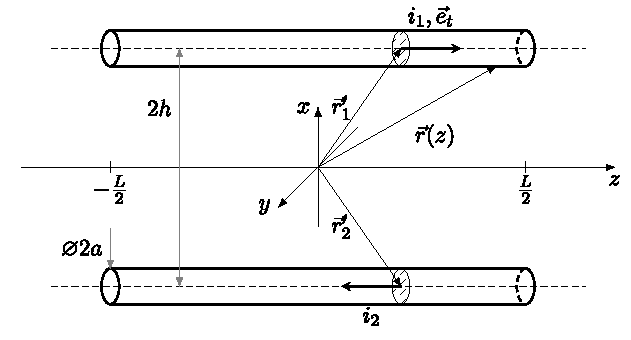
\includegraphics{res/LT17}
\end{center}
Der Aufpunktvektor $\vec{r}$ auf der Oberfläche des oberen Leiters bestimmt sich zu
\begin{equation}
	\vec{r}=(h-a) \vec{e}_{x}+z \vec{e}_{z} 
\end{equation}
während für die beiden Quellpunktvektoren $\vec{r}_{1}$ und $\vec{r}_{2}$ die Darstellung
\begin{equation}
	\vec{r}_{1 / 2}^{\prime}= \pm h \vec{e}_{x}+z^{\prime} \vec{e}_{z} 
\end{equation}
gilt. Die Abstände zum Aufpunkt bzw. die Beträge der beiden Differenzvektoren lauten folglich
\begin{align}
	& R_{1}:=\left|\vec{r}-\vec{r}_{1}\right|=\sqrt{a^{2}+\left(z-z^{\prime}\right)^{2}}  \\
	& R_{2}:=\left|\vec{r}-\vec{r}_{2}\right|=\sqrt{(2 h-a)^{2}+\left(z-z^{\prime}\right)^{2}} 
\end{align}
womit sich die Potentiale \ref{aleiter} und \ref{phileiter} in der Form (Achtung in $R_i$ steckt $z'$ drin)
\begin{align}
	 \ubar{\phi}(\vec{r})&=-\frac{\mathrm{j}}{4 \pi \varepsilon \omega} \int\limits_{-\frac{L}{2}}^{\frac{L}{2}}\left[\frac{\mathrm{e}^{-\mathrm{j} k R_{1}}}{R_{1}}-\frac{\mathrm{e}^{-\mathrm{j} k R_{2}}}{R_{2}}\right] \frac{\partial \ubar{I}\left(z^{\prime}\right)}{\partial z^{\prime}} \mathrm{d} z^{\prime}\label{LTform3}  \\
	\vec{\ubar{A}}(\vec{r})&=\frac{\mu}{4 \pi} \int\limits_{-\frac{L}{2}}^{\frac{L}{2}}\left[\frac{\mathrm{e}^{-\mathrm{j} k R_{1}}}{R_{1}}-\frac{\mathrm{e}^{-\mathrm{j} k R_{2}}}{R_{2}}\right] \ubar{I}\left(z^{\prime}\right) \vec{e}_{t}\left(z^{\prime}\right) \mathrm{d} z^{\prime} 
\end{align}
ausdrücken lassen. Mit der Randbedingung \ref{RBLT1} erhält man
\begin{equation}\begin{split}
	0=\vec{r}_{t}(z)(-\grad \ubar{\phi}-\mathrm{j} \omega \vec{\ubar{A}}) & =-\frac{\partial \ubar{\phi}}{\partial z}-\mathrm{j} \omega \vec{e}_{t}(z) \vec{\ubar{A}}  \\
	\frac{\partial \ubar{\phi}}{\partial z} & =-\mathrm{j} \omega \vec{e}_{t}(z) \vec{\ubar{A}} 
\end{split}\end{equation}
und kann somit schreiben
\begin{equation}\label{LTglsomit}
	\frac{\partial \ubar{\phi}}{\partial z}=-\mathrm{j} \omega \frac{\mu}{4 \pi} \int\limits_{-\frac{L}{2}}^{\frac{L}{2}}\left[\frac{\mathrm{e}^{-\mathrm{j} k R_{1}}}{R_{1}}-\frac{\mathrm{e}^{-\mathrm{j} k R_{2}}}{R_{2}}\right] \ubar{I}\left(z^{\prime}\right) \vec{e}_{t}(z) \vec{e}_{t}\left(z^{\prime}\right) \mathrm{d} z^{\prime} 
\end{equation}
Das Skalarprodukt der beiden Tangentialvektoren $\vec{e}_{t}(z) \vec{e}_{t}\left(z^{\prime}\right)$ innerhalb des Integrals ist dabei im allgemeinen Fall eines beliebig geformten Leiters ungleich Eins. Für das vorliegende Beispiel stimmen diese jedoch mit dem Einheitsvektor $\vec{e}_{z}$ überein und entfallen entsprechend. Durch Ausklammern von $\mathrm{e}^{-\mathrm{j} k R_{1}}$ vereinfacht man die Greensche Funktion im Integranden zu
\begin{equation}\label{greenfktintegrand}
	\frac{\mathrm{e}^{-\mathrm{j} k R_{1}}}{R_{1}}-\frac{\mathrm{e}^{-\mathrm{j} k R_{2}}}{R_{2}}=\mathrm{e}^{-\mathrm{j} k R_{1}}\left(\frac{1}{R_{1}}-\frac{\mathrm{e}^{-\mathrm{j} k\left(R_{2}-R_{1}\right)}}{R_{2}}\right) 
\end{equation}
Die Differenz der Abstände $R_{2}-R_{1}$ schätzt man nun unter Anwendung der Dreiecksungleichung $|\vec{a}-\vec{b}| \geq|\vec{a}|-|\vec{b}|$ zu
\begin{equation}
\begin{split}
	\left(\vec{r}-\vec{r}_{1}\right)-\left(\vec{r}-\vec{r}_{2}\right) & =-a \vec{e}_{x}+2 h \vec{e}_{x}+a \vec{e}_{x}=2 h \vec{e}_{x}  \\
	R_{2}-R_{1} & =\sqrt{(2 h-a)^{2}+\left(z-z^{\prime}\right)^{2}}-\sqrt{a^{2}+\left(z-z^{\prime}\right)^{2}} \leq 2 h 
\end{split}
\end{equation}
ab. Mit der Formulierung der Wellenzahl $k=\frac{2 \pi}{\lambda}$ und der Näherung $\lambda \gg 2 h$ kleiner Leiterabstände im Verhältnis zur Wellenlänge gilt für den Exponenten in Gleichung \ref{greenfktintegrand} also
\begin{equation}
	k\left(R_{2}-R_{1}\right) \leq \frac{2 \pi}{\lambda} 2 h=4 \pi \frac{h}{\lambda} \ll 1 
\end{equation}
Mithilfe die Reihenentwicklung des Exponentialterms gemäß
\begin{equation}
	\mathrm{e}^{x}=\sum_{k=0}^{\infty} \frac{x^{k}}{k!}=1+x+\frac{x^{2}}{2!}+\frac{x^{3}}{3!}+\ldots 
\end{equation}
wird deutlich, dass der Ausdruck $\mathrm{e}^{-\mathrm{j} k\left(R_{2}-R_{1}\right)} \approx 1$ ist. Das Integral in Gleichung \ref{LTglsomit} vereinfacht sich entsprechend
\begin{align}
	\int\limits_{-\frac{L}{2}}^{\frac{L}{2}}\left(\frac{1}{R_{1}}-\frac{1}{R_{2}}\right) \mathrm{e}^{-\mathrm{j} k R_{1}} \ubar{I}\left(z^{\prime}\right) \mathrm{d} z^{\prime} & \approx \int\limits_{-\frac{L}{2}}^{\frac{L}{2}}\left(\frac{1}{R_{1}}-\frac{1}{R_{2}}\right) \mathrm{e}^{-\mathrm{j} k a} \ubar{I}\left(z^{\prime}\right) \mathrm{d} z^{\prime}  \\
	& \stackrel{\mathrm{e}^{-\mathrm{j} k a} \approx 1}{\approx} \ubar{I}(z) \int\limits_{-\frac{L}{2}}^{\frac{L}{2}}\left(\frac{1}{R_{1}}-\frac{1}{R_{2}}\right) \mathrm{d} z^{\prime} 
\end{align}
Der letztere Näherungsschritt folgt dabei wiederum aus der Betrachtung für vergleichsweise große Wellenlängen, womit über große Leiterbereiche $z=z^{\prime}$ gilt und ein TEM-Mode der propagierenden Welle vorherrscht. Gleichfalls kann hierdurch der Leiterstrom bzw. die entsprechende Ableitung als konstant angenommen und aus der Integration gezogen werden. Die Spannung $\ubar{U}(z)$ an einer Stelle $z$ bestimmt sich letztlich aus der Potentialdifferenz zwischen den Leitern, wobei mit $\ubar{\phi}_{1}(z)=-\ubar{\phi}_{2}(z)$ (Symmetrie) die Relation
\begin{equation}
	\ubar{U}(z)=\ubar{\phi}_{1}(z)-\ubar{\phi}_{2}(z)=2 \ubar{\phi}_{1}(z) 
\end{equation}
folgt.
Aus \ref{LTglsomit} und \ref{LTform3} erhält man schließlich eine zu den Telegraphengleichungen äquivalente Darstellung der Form
\begin{align}
	 \frac{\partial \ubar{U}(z)}{\partial z}&=-\mathrm{j} \omega \underbrace{\frac{\mu}{2 \pi} \int_{-\frac{L}{2}}^{\frac{L}{2}}\left(\frac{1}{R_{1}}-\frac{1}{R_{2}}\right) \mathrm{d} z^{\prime} }_{=: L^{\prime}} \cdot \ubar{I}(z)  \\
	 \ubar{U}(z)&=\frac{\mathrm{j}}{2 \pi \varepsilon \omega} \int_{-\frac{L}{2}}^{\frac{L}{2}}\left(\frac{1}{R_{1}}-\frac{1}{R_{2}}\right) \mathrm{d} z^{\prime} \cdot \frac{\partial \ubar{I}(z)}{\partial z}  \\
	\rightarrow \quad \frac{\partial \ubar{I}(z)}{\partial z}&=-\mathrm{j} \omega 2 \pi \varepsilon \frac{1}{\underbrace{\int_{-\frac{L}{2}}^{\frac{L}{2}}\left(\frac{1}{R_{1}}-\frac{1}{R_{2}}\right) \mathrm{d} z^{\prime}}_{:=C^{\prime}}} \cdot \ubar{U}(z) 
\end{align}
mit $L^{\prime}$ als Induktivitätsbelag und $C^{\prime}$ als Kapazitätsbelag der Leitung. Im Falle eines unendlich langen Leiters mit $L \rightarrow \infty$ ergibt sich für jene Leitungsgrößen
\begin{align}
	L^{\prime} & =\frac{\mu}{2 \pi} \int_{-\infty}^{\infty}\left(\frac{1}{R_{1}}-\frac{1}{R_{2}}\right) \mathrm{d} z^{\prime}=\frac{\mu}{2 \pi} \ln \left(\frac{2 h}{a}\right)  \\
	C^{\prime} & =2 \pi \varepsilon\left[\int_{-\infty}^{\infty}\left(\frac{1}{R_{1}}-\frac{1}{R_{2}}\right) \mathrm{d} z^{\prime}\right]^{-1}=\frac{2 \pi \varepsilon}{\ln \left(\frac{2 h}{a}\right)} 
\end{align}



\iffalse\subsection{Klassische Leitungstheorie}\label{leitungstheorie}
\begin{itemize}
	\item Die \textbf{klassische Leitungstheorie} dient der Beschreibung von \textbf{langen Leitungen} mittels \textbf{Strom und Spannung}.
	\item Von einer \textbf{langen Leitung} spricht man, wenn die Länge der Leitung nicht mehr als klein im Vergleich zur \textbf{Wellenlänge} angesehen werden kann.
	\centerline{%
		\begin{tabular}{c||c|c|c|c|c|c}
			$f$                                   & $50\mathrm{Hz}$      & $1\mathrm{kHz}$    & $100\mathrm{MHz}$ & $1\mathrm{GHz}$   & $10\mathrm{GHz}$ \\
			\hline
			$\lambda_{\text{Vakuum}}=\frac{c}{f}$ & $5995.8 \mathrm{km}$ & $299.8\mathrm{km}$ & $2.99\mathrm{m}$  & $29.9\mathrm{cm}$ & $2.9\mathrm{cm}$
	\end{tabular}}
	\item Im einfachsten Fall wird die Leitung als \textbf{verlustlose, homogene Einfachleitung} angesehen. Es handelt sich also um einen \textbf{zylindrischen Wellenleiter}.
	\item Das Querschnittsgebiet ist \textbf{nicht einfach zusammenhängend} und daher existiert ein (quasi) {TEM-Mode}.
	\item Nur der TEM-Mode wird betrachtet: daher kann mit \textbf{Spannungen in der Transversalebene} gerechnet werden.
	\item Verallgemeinerungen bis hin zu einer \textbf{full-wave} Beschreibung sind möglich!
	\item Beispielstrukturen, die gerne mit Leitungstheorie beschrieben werden: Koaxialkabel, Zweidrahtleitung, Mikrostreifenleitung
\end{itemize}
\subsection{Ausgangspunkt}
\begin{itemize}
	\item Ziel ist die Entwicklung eines \textbf{Ersatzschaltbilds} für ein \textbf{differentielles Leitungselement}.
	\item Ausgangspunkt ist feldtheoretische Beschreibung für den \textbf{verlustlosen Fall}.
	\item Das Ersatzschaltbild kann dann einfach \textbf{verallgemeinert} werden.
	\item Maxwellgleichungen (lin. hom. iso. Dielektrikum, harmonische ZA, keine Quellen):
	\begin{align}
		\div \ubar{\vec{E}} & = 0 & \rot \ubar{\vec{E}} + \mathrm{j}\omega\mu \vec{\ubar{H}}         & =\vec{0} \\
		\div \vec{\ubar{H}} & = 0 & \rot \vec{\ubar{H}} - \mathrm{j}\omega\varepsilon \ubar{\vec{E}} & =\vec{0}
	\end{align}
	\item Wir betrachten nur den \textbf{TEM-Mode}. Die \textbf{Ausbreitungsrichtung} sei \(\pm\vu{z}\). Es gilt:
	\begin{align}
		\text{TEM-Mode: } &  & \ubar{\vec{E}}\cdot \vu{z}                    & =0                                           & \vec{\ubar{H}}\cdot \vu{z}                    & =0                                           \\
		&  & \left( \rot \ubar{\vec{E}}\right)\times\vu{z} & = \frac{\partial \ubar{\vec{E}}}{\partial z} & \left( \rot \vec{\ubar{H}}\right)\times\vu{z} & = \frac{\partial \vec{\ubar{H}}}{\partial z}
	\end{align}
	\begin{equation}
		\text{Transversalebene: }  \rot _t\ubar{\vec{E}} = \left( \frac{\partial \ubar{E}_y}{\partial x}-\frac{\partial \ubar{E}_x}{\partial y}\right)\vu{z} \Rightarrow\left(\rot _t\ubar{\vec{E}}\right)\cdot\vu{x,y} =0
	\end{equation}
\end{itemize}
\subsection{Felder -- Transversalebene (\(z=\text{const.}\))}
\begin{itemize}
	\item Transversalkomponente des Induktionsgesetztes (in der Transversalebene):
	\begin{align}
		\rot \ubar{\vec{E}} + \mathrm{j}\omega\mu\vec{\ubar{H}} & =\vec{0} \Rightarrow & \left(\rot \ubar{\vec{E}}\right)\times\vu{z} + \mathrm{j}\omega\mu\vec{\ubar{H}} \times\vu{z}       & =\vec{0}  \\
		&                      & \Aboxed{\frac{\partial \ubar{\vec{E}}}{\partial z} + \mathrm{j}\omega\mu\vec{\ubar{H}} \times\vu{z} & =\vec{0}}
	\end{align}
	\item Das elektrische Feld ist ein \textbf{Gradientenfeld} in allen Transversalebenen. Ansatz:
	\begin{equation}
		\boxed{\ubar{\vec{E}} = -\grad \phi(x,y) \; g(z)} \text{ mit } \boxed{\Delta \phi(x,y) = 0} \text{ statische 2D Laplace Gleichung}
	\end{equation}
	\item Magnetfeld direkt ausrechnen:
	\begin{align}
		\frac{\partial \ubar{\vec{E}}}{\partial z} + \mathrm{j}\omega\mu\vec{\ubar{H}} \times\vu{z} & =\vec{0} & \Rightarrow \vu{z}\times\frac{\partial \ubar{\vec{E}}}{\partial z} & + \mathrm{j}\omega\mu\, \vu{z}\times\left(\vec{\ubar{H}} \times\vu{z}\right) =\vec{0}                \\
		&          & \vec{\ubar{H}}                                                     & = -\frac{1}{\mathrm{j}\omega\mu} \left(\vu{z}\times\frac{\partial \ubar{\vec{E}}}{\partial z}\right) \\
		&          & \Aboxed{\vec{\ubar{H}}                                             & = \frac{1}{\mathrm{j}\omega\mu} \left(\vu{z}\times\grad \phi\right)\frac{\partial g}{\partial z}}
	\end{align}
\end{itemize}
\subsection{Übergang zu Strom und Spannung}
\begin{center}
	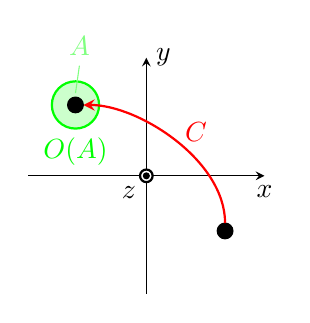
\begin{tikzpicture}
	\draw[thin,-stealth] (-1.5,0) -- (+1.5,0) node[below]{$x$};
	\draw[thin,-stealth] (0,-1.5) -- (0,+1.5) node[right]{$y$};
	\draw[fill=black] (1,-0.7) circle (0.1);
	\draw[fill=green!20,draw=green,thick] (-0.9,0.9) circle (0.3) node[color=green,below,yshift=-8]{$O(A)$};
	\draw[fill=black] (-0.9,0.9) circle (0.1);
	\draw[thick,red,-stealth] (1,-0.6) .. controls (1,.2) and (-0.1,0.9) .. (-0.8,0.9) node[midway,right,yshift=3] {$C$};
	\draw[color=green!50] (-0.9,1.05) -- (-0.85,1.4) node[color=green!50,above]{$A$};
	\draw[thick, fill=white] (0,0) circle (0.08) node[anchor=north east]{$z$};
	\draw[thick, fill=black] (0,0) circle (0.03);
\end{tikzpicture}
\end{center}

\begin{itemize}
	\item Stromdichte konstant im Leiterquerschnitt \(\to\) \textbf{Dünndrahtnäherung}
	\item Perfekte Leiter: \(\kappa \to \infty\)
	\item Rotationsfreiheit des elektrischen Felds in der Transversalebene \(\to\) \textbf{Spannung}:
	\begin{equation}
		\ubar{U} = \int\limits_C \ubar{\vec{E}} \cdot \dd \vec{s} \; \text{ mit \(z =\) const. auf \(C\)}
	\end{equation}
	\item Aus dem Durchflutungsgesetz \(\to\) \textbf{Strom:}
	\begin{equation}
		\ubar{I} = \oint\limits_{O(A)} \vec{\ubar{H}} \cdot \dd\vec{s}
	\end{equation}
\end{itemize}

\begin{itemize}
	\item Damit können die Ausdrücke für die Felder umgeformt werden:
	\begin{equation}
		\frac{\partial \ubar{\vec{E}}}{\partial z} + \mathrm{j}\omega\mu\vec{\ubar{H}} \times\vu{z} =\vec{0} \quad\text{und}\quad \vec{\ubar{H}}= \frac{1}{\mathrm{j}\omega\mu} \left(\vu{z}\times\grad \phi\right)\frac{\partial g}{\partial z}
	\end{equation}
	\item Ausdrücke für die Felder:
	\begin{equation}
		\frac{\partial \ubar{\vec{E}}}{\partial z} + \mathrm{j}\omega\mu\vec{\ubar{H}} \times\vu{z} =\vec{0} \quad\text{und}\quad \vec{\ubar{H}}= \frac{1}{\mathrm{j}\omega\mu} \left(\vu{z}\times\grad \phi\right)\frac{\partial g}{\partial z}
	\end{equation}
	\item Wir bilden das Wegintegral der ersten Gleichung entlang \(C\) und setzen dann \(\vec{\ubar{H}}\) ein:
	\begin{equation}\begin{split}
			\int\limits_C \frac{\partial \ubar{\vec{E}}}{\partial z} \cdot \dd \vec{s} + \mathrm{j}\omega\mu \int\limits_C\left(\vec{\ubar{H}} \times\vu{z}\right) \cdot \dd \vec{s} &= 0  \\
			\Aboxed{\frac{\partial  \ubar{U}}{\partial z} + \frac{\partial g}{\partial z} \int\limits_C\grad \phi \cdot \dd \vec{s} = 0}
	\end{split}\end{equation}
	\item Weiter gilt für den Strom:
	\begin{align}
		II = \oint\limits_{O(A)} \vec{\ubar{H}} \cdot \dd\vec{s} & = \oint\limits_{O(A)} \frac{1}{\mathrm{j}\omega\mu} \left(\vu{z}\times\grad \phi\right)\frac{\partial g}{\partial z} \cdot \dd\vec{s} \\
		\Rightarrow \Aboxed{\frac{\partial g}{\partial z}        & = \mathrm{j}\omega\mu \frac{ \ubar{I}}{\oint\limits_{O(A)} \left(\vu{z}\times\grad \phi\right) \cdot \dd\vec{s}}}
	\end{align}
	\item Wir betrachten die Formeln
	\begin{equation}
		\frac{\partial  \ubar{U}}{\partial z} + \frac{\partial g}{\partial z} \int\limits_C\grad \phi \cdot \dd \vec{s} = 0 \text{ und } \frac{\partial g}{\partial z} = \mathrm{j}\omega\mu \frac{ \ubar{I}}{\oint\limits_{O(A)} \left(\vu{z}\times\grad \phi\right) \cdot \dd\vec{s}}
	\end{equation}
	\item Einsetzen der rechten in die linke Gleichung eliminiert offensichtlich die unbekannte Funktion \(g(z)\) und wie erhalten die \textbf{erste Leitungsgleichung} (Telegraphengleichung):
	\begin{equation}
		\frac{\partial  \ubar{U}(z)}{\partial z} + \mathrm{j}\omega \underbrace{\frac{\mu\int\limits_C\grad \phi \cdot \dd \vec{s}}{\oint\limits_{O(A)} \left(\vu{z}\times\grad \phi\right) \cdot \dd\vec{s}}}_{L^\prime}  \ubar{I}(z)=\boxed{\frac{\partial  \ubar{U}(z)}{\partial z} + \mathrm{j}\omega L^\prime  \ubar{I}(z)= 0} \quad [L^\prime] = \mathrm{\frac{H}{m}}
	\end{equation}
	\item Der \textbf{Induktivitätsbelag} der Leitung \(L^\prime\) ist vollständig bestimmt durch die Lösung des statischen 2D Laplace-Randwertproblems für \(\phi\) im Lösungsvolumen \(V\)
	\begin{equation}
		\Delta \phi(x,y) = 0 \text{ mit }  \phi = 0 \text{ auf einem Leiter und } \phi =  U(z) \text{ auf dem anderen Leiter}
	\end{equation}
	
	\item Analog folgt die \textbf{zweite Leitungsgleichung} aus den Formeln:
	\begin{equation}
		\frac{\partial \vec{\ubar{H}}}{\partial z} - \mathrm{j}\omega\varepsilon\ubar{\vec{E}} \times\vu{z} =\vec{0} \text{ und } \ubar{\vec{E}} = -\grad \phi \; g(z)
	\end{equation}
	\item Umlaufintegral der ersten Gleichung entlang \(O(A)\) und Einsetzen von \(\ubar{\vec{E}}\) ergibt:
	\begin{equation}\begin{split}
			\oint\limits_{O(A)} \frac{\partial \vec{\ubar{H}}}{\partial z} \cdot \dd \vec{s} - \mathrm{j}\omega\varepsilon \oint\limits_{O(A)}\left(\ubar{\vec{E}} \times\vu{z}\right) \cdot \dd \vec{s} &= 0  \\
			\frac{\partial  \ubar{I}}{\partial z} -\mathrm{j}\omega\varepsilon\; g(z) \oint\limits_{O(A)}\left(\vu{z}\times \grad \phi\right) \cdot \dd \vec{s} &= 0
	\end{split}\end{equation}
	\item Die Funktion \(g(z)\) folgt sofort aus \( \ubar{U}\):
	\begin{equation}
		\ubar{U} = \int\limits_C \ubar{\vec{E}}\cdot\dd\vec{s} = -g(z) \int\limits_C \grad \phi\cdot\dd\vec{s} \to g(z) = -\frac{ \ubar{U}}{\int\limits_C \grad \phi\cdot\dd\vec{s}}
	\end{equation}
	\item Damit lautet die \textbf{zweite Leitungsgleichung}:
	\begin{equation}
		\frac{\partial  \ubar{I}}{\partial z} +\mathrm{j}\omega \underbrace{\frac{\varepsilon\oint\limits_{O(A)}\left(\vu{z}\times \grad \phi\right) \cdot \dd \vec{s}}{\int\limits_C \grad \phi\cdot\dd\vec{s}}}_{C^\prime}  \ubar{U} = 0 \quad [C^\prime]=\mathrm{\frac{F}{m}}
	\end{equation}
\end{itemize}
\subsection{Leitungsgleichungen -- Leitungsbeläge}
\begin{itemize}
	\item Zusammenfassend haben wir für verlustlose Leitungen die folgenden \textbf{Leitungsgleichungen} gefunden:
	\begin{align}
		\frac{\partial  \ubar{U}(z)}{\partial z} + \mathrm{j}\omega L^\prime  \ubar{I}(z) & = 0 & L^\prime & =\frac{\mu\int\limits_C\grad \phi \cdot \dd \vec{s}}{\oint\limits_{O(A)} \left(\vu{z}\times\grad \phi\right) \cdot \dd\vec{s}}         \\
		\frac{\partial  \ubar{I}(z)}{\partial z} +\mathrm{j}\omega C^\prime  \ubar{U}(z)  & = 0 & C^\prime & = \frac{\varepsilon\oint\limits_{O(A)}\left(\vu{z}\times \grad \phi\right) \cdot \dd \vec{s}}{\int\limits_C \grad \phi\cdot\dd\vec{s}}
	\end{align}
	\item Offensichtlich gilt
	\begin{equation}
		L^\prime C^\prime = \varepsilon\mu = \frac{1}{ v_\mathrm{p}^2} \Rightarrow \boxed{ v_\mathrm{p} = \frac{1}{\sqrt{L^\prime C^\prime}}}
	\end{equation}
	\item Entkoppelte Gleichungen:
	\begin{equation}
		\frac{\partial^2  \ubar{U}(z)}{\partial z^2} + \omega^2 L^\prime C^\prime  \ubar{U}(z) = 0 \text{ und } \frac{\partial^2  \ubar{I}(z)}{\partial z^2} + \omega^2 L^\prime C^\prime  \ubar{I}(z) = 0
	\end{equation}
	\item Die Lösungen sind (natürlich) vor- und zurücklaufende Wellen (als ruhende Zeiger):
	\begin{equation}
		\ubar{U}(z) =  \ubar{U}_0  \mathrm{e}^{\pm\mathrm{j}kz} \text{ und }  \ubar{I}(z) =  \ubar{I}_0  \mathrm{e}^{\pm\mathrm{j}kz}
	\end{equation}
\end{itemize}
\subsection{Übergang zum Ersatzschaltbild}
\begin{center}
	\ctikzset{voltage/bump b=1.1}
\begin{circuitikz}[european voltages,scale=.75]
	\draw (0,0) to[short,o-o] (4,0);
	\draw (0,2) to [short, i=$\ubar{I}(z)$,o-] (1,2) to[L=L,-] (3,2) coordinate(a);
	\draw (a) to[short, i=$\ubar{I}(z+\Delta z)$,-o]  (4,2);
	\draw (a) to[C,l_=C,*-*] ++(0,-2);

	% Voltage labels
	\draw (0,2) to[open,v=$\ubar{U}(z)$] ++(0,-2);
	\draw (4,2) to[open, v^=$\ubar{U}(z+\Delta z)$] ++(0,-2);
\end{circuitikz}
\end{center}

\begin{itemize}
	\item Maschensatz:
	\begin{equation}\begin{split}
			\ubar{U}(z) = \mathrm{j}\omega L  \ubar{I}(z) +  \ubar{U}(z+\Delta z)\\
			\ubar{U}(z+\Delta z) - \ubar{U}(z) + \mathrm{j}\omega L  \ubar{I}(z) =0  \\
			\frac{\Delta  \ubar{U}}{\Delta z} + \mathrm{j}\omega \frac{L}{\Delta z}  \ubar{I}(z) =0
	\end{split}\end{equation}
	
	\item Knotensatz:
	\begin{equation}
		\ubar{I}(z+\Delta z) =  \ubar{I}(z) - \mathrm{j}\omega C  \ubar{U}(z+\Delta z) \Rightarrow \frac{\Delta  \ubar{I}}{\Delta z} + \mathrm{j}\omega \frac{C}{\Delta z}  \ubar{U}(z+\Delta z) = 0
	\end{equation}
	\item Im Grenzfall \(\Delta z \to 0\) und mit \(C^\prime=\lim_{\Delta z \to 0} \frac{C}{\Delta z}\) und \(L^\prime=\lim_{\Delta z \to 0} \frac{L}{\Delta z}\) ist der obige Vierpol das \textbf{Ersatzschaltbild eines differentiellen Stückes einer verlustlosen Leitung.}
	\item Verallgemeinerung für \textbf{verlustbehaftete} Leitungen:
	\begin{center}
		\ctikzset{voltage/bump b=1.1}
\ctikzset{bipoles/length=.7cm}
\begin{circuitikz}[european voltages,scale=.75]
	\draw (0,0) to[short,o-o] (7,0);
	\draw (0,1.5) to [short, i=$\ubar{I}(z)$,o-] (1,1.5) to[R=$R^\prime \dd z$] (2,1.5) to[L=$L^\prime \dd z$,-] (4,1.5) coordinate(a);
	\draw (a) to[short, -] (5,1.5) coordinate(b);
	\draw (b) to[short, i=$\ubar{I}(z+\dd z)$,-o]  (7,1.5);
	\draw (a) to[C,l_=$C^\prime \dd z$,*-*] ++(0,-1.5);
	\draw (b) to[R,l=$G^\prime \dd z$,*-*] ++(0,-1.5);

	% Voltage labels
	\draw (0,1.5) to[open,v=$\ubar{U}(z)$] ++(0,-1.5);
	\draw (7,1.5) to[open, v^=$\ubar{U}(z+\dd z)$] ++(0,-1.5);
\end{circuitikz}
	\end{center}
	
\end{itemize}
\subsection{Verlustbehaftete Leitungen}
\begin{itemize}
	\item Aus dem Ersatzschaltbild ergeben sich die \textbf{Leitungsgleichungen für verlustbehaftete Leitungen}.
	\begin{align}
		\frac{\partial  \ubar{U}(z)}{\partial z} + \left(R^\prime + \mathrm{j}\omega L^\prime\right)  \ubar{I}(z) & = 0 & L^\prime & =\frac{\mu\int\limits_C\grad \phi \cdot \dd \vec{s}}{\oint\limits_{O(A)} \left(\vu{z}\times\grad \phi\right) \cdot \dd\vec{s}}         \\
		\frac{\partial  \ubar{I}(z)}{\partial z} +\left(G^\prime + \mathrm{j}\omega C^\prime\right)  \ubar{U}(z)  & = 0 & C^\prime & = \frac{\varepsilon\oint\limits_{O(A)}\left(\vu{z}\times \grad \phi\right) \cdot \dd \vec{s}}{\int\limits_C \grad \phi\cdot\dd\vec{s}}
	\end{align}
	\item Der \textbf{Widerstandsbelag} \(R^\prime\) entspricht den ohmschen Leitungsverlusten pro Längeneinheit.
	\item Der \textbf{Leitwertbelag} \(G^\prime\)  entspricht den dielektrischen Verlusten pro Längeneinheit.
	\item Zusammengefasst spricht man auch vom \textbf{Impedanzbelag} \(Z^\prime = R^\prime + \mathrm{j}\omega L^\prime\) und vom \textbf{Admittanzbelag} \(Y^\prime = G^\prime + \mathrm{j}\omega C^\prime\)
\end{itemize}
\subsection{Allgemeine Lösung -- Leitungswellenwiderstand}
\begin{itemize}
	\item Wir können die entkoppelten Leitungsgleichungen jetzt auch allgemein hinschreiben:
	\begin{equation}
		\frac{\partial^2  \ubar{U}(z)}{\partial z^2} -  Z^\prime Y^\prime  \ubar{U}(z) = 0 \text{ und } \frac{\partial^2  \ubar{I}(z)}{\partial z^2} -  Z^\prime Y^\prime  \ubar{I}(z) = 0
	\end{equation}
	\item Ansatz:
	\begin{equation}
		\ubar{U}(z) = u  \mathrm{e}^{\pm\ubar{\gamma} z} \Rightarrow \ubar{\gamma} = \sqrt{Z^\prime Y^\prime} = \sqrt{\left(R^\prime + \mathrm{j}\omega L^\prime\right) \left(G^\prime + \mathrm{j}\omega C^\prime\right)} \text{ Ausbreitungskonstante}
	\end{equation}
	\item Mit der Spannung \( \ubar{U}(z) = u_1  \mathrm{e}^{-\ubar{\gamma} z} + u_2  \mathrm{e}^{\ubar{\gamma} z}\) ergibt sich der Strom zu
	\begin{equation}
		\ubar{I}(z) = - \frac{1}{Z^\prime} \frac{\partial  \ubar{U}(z)}{\partial z} = \frac{\ubar{\gamma}{Z^\prime} \left( u_1  \mathrm{e}^{-\ubar{\gamma} z} - u_2  \mathrm{e}^{\ubar{\gamma} z}\right) = \frac{1}{Z_L} \left( u_1  \mathrm{e}^{-\ubar{\gamma} z} - u_2  \mathrm{e}^{\ubar{\gamma} z}\right)
	\end{equation}
	\item Hierbei ist \(Z_L\) der \textbf{Leitungswellenwiderstand}:
	\begin{equation}
		Z_L= \frac{Z^\prime}{\ubar{\gamma} = \sqrt{\frac{Z^\prime}{Y^\prime}} = \sqrt{\frac{R^\prime + \mathrm{j}\omega L^\prime}{G^\prime + \mathrm{j}\omega C^\prime}}
	\end{equation}
	\item Abschluss mit Leitungswellenwiderstand \(\to\) Eingangsimpedanz = Leitungswellenwiderstand \(\to\) \textbf{keine Reflexion}
\end{itemize}
\subsection{Matrixschreibweise -- Mehrfachleitungen}
\begin{itemize}
	\item Die gefundenen Leitungsgleichungen werden üblicherweise in eine \textbf{Matrixgleichung} zusammengefasst:
	\begin{equation}
		\left.
		\begin{array}{rl}
			\frac{\partial  \ubar{U}(z)}{\partial z} + \left(R^\prime + \mathrm{j}\omega L^\prime\right)  \ubar{I}(z) & = 0 \\
			\frac{\partial  \ubar{I}(z)}{\partial z} +\left(G^\prime + \mathrm{j}\omega C^\prime\right)  \ubar{U}(z)  & = 0
		\end{array}\right\} \Rightarrow
		\frac{\partial}{\partial z}\begin{pmatrix} \ubar{U}(z)\\ \ubar{I}(z) \end{pmatrix}
		+
		\begin{pmatrix}
			0        & Z^\prime \\
			Y^\prime & 0
		\end{pmatrix}
		\begin{pmatrix} \ubar{U}(z)\\ \ubar{I}(z) \end{pmatrix} = 0
	\end{equation}
	\item Die Matrixgleichung ist sofort für \textbf{Mehrfachleitungen} verallgemeinbar. Hierzu bilden wir
	\begin{itemize}
		\item den Vektor der Spannungen relativ zum Bezugsleiter \(\vec{ \ubar{U}}(z) = \left( \ubar{U}_1(z),\ldots ,  \ubar{U}_n(z) \right)^T\).
		\item den Vektor der Ströme im Leiter  \(\vec{ \ubar{I}}(z) = \left( \ubar{I}_1(z),\ldots ,  \ubar{I}_n(z) \right)^T\).
		\item die Matrix mit den Impedanzbelägen in der Hauptdiagonalen \(\left(Z^\prime\right)\)
		\item die Matrix mit den Admittanzbelägen in der Hauptdiagonalen \(\left(Y^\prime\right)\)
		\begin{equation}
			\frac{\partial}{\partial z}\begin{pmatrix}\vec{ \ubar{U}}(z)\\\vec{ \ubar{I}}(z) \end{pmatrix}
			+
			\begin{pmatrix}
				0                            & \left(Z^\prime\right) \\
				\left(Y^\prime\right)^\prime & 0
			\end{pmatrix}
			\begin{pmatrix}\vec{ \ubar{U}}(z)\\\vec{ \ubar{I}}(z) \end{pmatrix} = 0
		\end{equation}
		
	\end{itemize}
\end{itemize}
\subsection{Bemerkungen}
\begin{itemize}
	\item Die Leitungstheorie kann hier nur angerissen werden.
	\item Die Anwendungen sind extrem vielfältig: Beschreibung von Leitungen, Impedanztransformationen, Anpassungen, Filter, \dots
	\item Vierpolparameter: Z, S, Y \(\to\) bekannt aus Grundlagen (Vierpole)
	\item \textbf{Ungleichförmige Leitungen}: ortsabhängigen Leitungsbeläge
	\item Wichtigste Einschränkung der klassischen Leitungstheorie: \textbf{nur TEM-Mode}
	\item Deshalb auch: Abstrahlung und Einkopplung in Leitungen nur bedingt beschreibbar.
	\item Lösung: \textbf{Transmission Line Super Theory (TLST)}, z.B. F. Ossevorth, R. Jacobs, H.G. Krauthäuser,
	\enquote{A full wave description for thin wire structures with TLST and perturbation theory}, Advances in Radio Science (16), 123--133, 2018. \url{https://ars.copernicus.org/articles/16/123/2018/}, DOI = 10.5194/ars-16-123-2018 und dort zitierte Arbeiten (insbesondere: S. Tkachenko und J. Nitsch)
\end{itemize}
\subsection{Netzwerkbeschreibung mithilfe der Baum-Liu-Tesche-Gleichung}
Neben der Beschreibung von Leitungen mit den Telegrafengleichungen besteht ebenfalls die Möglichkeit der Modellierung eines Netzwerkes unter Nutzung der sogenannten Baum-Liu-Tesche-Gleichung (benannt nach Begründern, kurz BLT-Gleichung). Hierbei werden Leitungen an ihren Abschlüssen ausgewertet, sodass eine umfassende Berechnung komplexer Netzwerke möglich ist.

Man betrachte das folgende Netzwerk mit einer Spannungs- oder einer Stromeinkopplung $U_{0}$ bzw. $I_{0}$ an einer beliebigen Stelle $z_{\mathrm{S}}$ der Leitung.

\begin{center}
	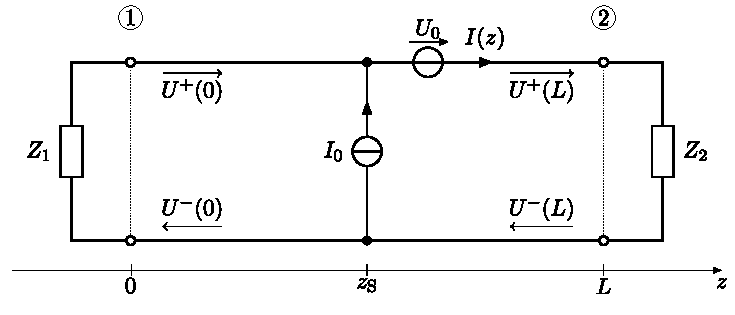
\includegraphics{res/LT6}
\end{center}

Darin bezeichnen die eingezeichneten Spannungen $U^{+}(0)=U_{1}^{\text {refl }}$ und $U^{-}(0)=U_{1}^{\text {inc }}$ die reflektierte und in positive $z$-Richtung propagierende bzw. die inzidente und in negative $z$-Richtung laufende Welle am Leitungsanfang (Tor 1) bei $z=0$. Gleichermaßen stellen $U^{+}(L)=U_{2}^{\text {inc }}$ und $U^{-}(L)=U_{2}^{\text {refl }}$ die inzidente bzw. reflektierte Welle am Leitungsende bei $z=L$ (Tor 2) dar.

Zunächst soll zur Berechnung der Spannung $U(z)$ an einer Stelle $z$ der Leitung mit konzentrierten Schaltungselementen gerechnet werden. Die dargestellten Impedanzen $Z_{1}$ und $Z_{2}$ sind dabei entsprechend als zusammengefasste Leitungsimpedanzen der Übertragungsleitung aufzufassen. Als Ansatz für die Spannung am Ort $z \in\left[z_{S} ; L\right]$ wählt man nun die Superposition einer in $z$-Richtung fortschreitenden und einer am Leitungsende reflektierten und in entgegengesetzte Richtung laufenden Welle gemäß


\begin{equation}\label{LTreflwell}
	U(\tilde{z})=\left(\tilde{U}+Z_{\mathrm{C}} \tilde{I}\right)\left(\mathrm{e}^{-\ubar{\gamma} \tilde{z}}+r_{2} \mathrm{e}^{+\ubar{\gamma} \tilde{z}}\right) \quad \text { für } \quad z_{\mathrm{S}}-L \leq \tilde{z} \leq 0 
\end{equation}


mit der Notation $\tilde{z}=z-L=-(L-z)$. Der vorangestellte Klammerterm ist ein konstanter Vorfaktor, welcher die noch unbekannten Integrationskonstanten $\tilde{U}$ und $\tilde{I}$ als Wirkung der beiden Anregungsquellen beinhaltet. Diese lassen sich aus den Randbedingungen am Erregungsort bestimmen, wobei die auftretende Gesamtspannung als Summe der Spannungswirkungen von Spannungs- und Stromquelle durch


\begin{equation}
	U\left(z_{\mathrm{S}}-L\right)=\underbrace{U_{1}\left(z_{\mathrm{S}}-L\right)}_{\text {Spannungsquelle }}+\underbrace{U_{2}\left(z_{\mathrm{S}}-L\right)}_{\text {Stromquelle }} 
\end{equation}


ausgedrückt und die Spannungs- bzw. Stromteilerregel zur Lösung angewendet wird. Für ersteren Summanden gilt dann


\begin{equation}\label{summand1LT}
	U_{1}\left(z_{\mathrm{S}}-L\right)=\tilde{U}\left(\mathrm{e}^{-\ubar{\gamma}\left(z_{\mathrm{S}}-L\right)}+r_{2} \mathrm{e}^{+\ubar{\gamma}\left(z_{\mathrm{S}}-L\right)}\right)=U_{0} \frac{Z_{2}}{Z_{1}+Z_{2}} 
\end{equation}

mit den Leitungsimpedanzen


\begin{equation}
	Z_{1}=\frac{U\left(z_{\mathrm{S}}\right)}{I\left(z_{\mathrm{S}}\right)}=Z_{\mathrm{C}} \frac{1+r_{1} \mathrm{e}^{-2 \ubar{\gamma} z_{\mathrm{S}}}}{1-r_{1} \mathrm{e}^{-2 \ubar{\gamma} z_{\mathrm{S}}}} \quad \text { und } \quad Z_{2}=\frac{U\left(z_{\mathrm{S}}-L\right)}{I\left(z_{\mathrm{S}}-L\right)}=Z_{\mathrm{C}} \frac{1+r_{2} \mathrm{e}^{2 \ubar{\gamma}\left(z_{\mathrm{S}}-L\right)}}{1-r_{2} \mathrm{e}^{2 \ubar{\gamma}\left(z_{\mathrm{S}}-L\right)}} 
\end{equation}


für die Abschnitte links und rechts der Einkopplung. Somit erhält man aus \ref{summand1LT} den Ausdruck


\begin{equation}
	\frac{\tilde{U}}{U_{0}}=\frac{Z_{2}}{Z_{1}+Z_{2}} \cdot \frac{1}{\mathrm{e}^{-\ubar{\gamma}\left(z_{\mathrm{s}}-L\right)}+r_{2} \mathrm{e}^{+\ubar{\gamma}\left(z_{\mathrm{s}}-L\right)}} 
\end{equation}


Analog folgt für den zweiten Summanden


\begin{align}
	U_{2}\left(z_{\mathrm{S}}-L\right) & =Z_{\mathrm{C}} \tilde{I}\left(\mathrm{e}^{-\ubar{\gamma}\left(z_{\mathrm{s}}-L\right)}-r_{2} \mathrm{e}^{+\ubar{\gamma}\left(z_{\mathrm{S}}-L\right)}\right)=Z_{\mathrm{C}} I_{0} \cdot \frac{Z_{1}}{Z_{1}+Z_{2}}  \\
	\frac{\tilde{I}}{I_{0}} & =\frac{Z_{1}}{Z_{1}+Z_{2}} \cdot \frac{1}{\mathrm{e}^{-\ubar{\gamma}\left(z_{\mathrm{s}}-L\right)}+r_{2} \mathrm{e}^{+\ubar{\gamma}\left(z_{\mathrm{S}}-L\right)}} 
\end{align}


Die Konstanten bestimmt man damit zu


\begin{align}
	& \tilde{U}=U_{0} \frac{\frac{1+r_{2} \mathrm{e}^{2 \ubar{\gamma}\left(z_{\mathrm{S}}-L\right)}}{1-r_{2} \mathrm{e}^{\ubar{\gamma} \ubar{\gamma}\left(z_{\mathrm{s}}-L\right)}}}{\frac{1+r_{1} \mathrm{e}^{-2 \ubar{\gamma} z_{\mathrm{S}}}}{1-r_{1} \mathrm{e}^{-2 \ubar{\gamma} z_{\mathrm{S}}}}+\frac{1+r_{2} \mathrm{e}^{2 \ubar{\gamma}\left(z_{\mathrm{S}}-L\right)}}{1-r_{2} \mathrm{e}^{2 \ubar{\gamma}\left(z_{\mathrm{S}}-L\right)}}} \cdot \frac{1}{\mathrm{e}^{-\ubar{\gamma}\left(z_{\mathrm{S}}-L\right)}+r_{2} \mathrm{e}^{+\ubar{\gamma}\left(z_{\mathrm{S}}-L\right)}}  \\
	& =\ldots=U_{0} \frac{1-r_{1} \mathrm{e}^{-2 \ubar{\gamma} z_{\mathrm{S}}}}{2\left(1-r_{1} r_{2} \mathrm{e}^{-2 \ubar{\gamma} L}\right)} \mathrm{e}^{\ubar{\gamma}\left(z_{\mathrm{S}}-L\right)}  \\
	& \tilde{I}=I_{0} \frac{1+r_{1} \mathrm{e}^{-2 \ubar{\gamma} z_{\mathrm{S}}}}{2\left(1-r_{1} r_{2} \mathrm{e}^{-2 \ubar{\gamma} L}\right)} \mathrm{e}^{\ubar{\gamma}\left(z_{\mathrm{S}}-L\right)} 
\end{align}


Einsetzen in die Ausgangsgleichung \ref{LTreflwell} führt auf einen Ausdruck für die Spannung und den Strom im Bereich zwischen Erregungsort $z=z_{\mathrm{S}}$ und Port 2 bei $z=L$


\begin{align}
	U(z) & =\frac{\mathrm{e}^{-\ubar{\gamma} z}+r_{2} \mathrm{e}^{\ubar{\gamma}(z-2 L)}}{2\left(1-r_{1} r_{2} \mathrm{e}^{-2 \ubar{\gamma} L}\right)}\left[U_{0}\left(\mathrm{e}^{\ubar{\gamma} z \mathrm{~s}}-r_{1} \mathrm{e}^{-\ubar{\gamma} z \mathrm{~s}}\right)+Z_{\mathrm{C}} I_{0}\left(\mathrm{e}^{\ubar{\gamma} z \mathrm{~s}}+r_{1} \mathrm{e}^{-\ubar{\gamma} z \mathrm{~s}}\right)\right]  \\
	I(z) & =\frac{1}{Z_{\mathrm{C}}}\left(\tilde{U}^{+} \mathrm{e}^{-\ubar{\gamma} \tilde{z}}-\tilde{U}^{-} \mathrm{e}^{+\ubar{\gamma} \tilde{z}}\right)  \\
	& =\frac{\mathrm{e}^{-\ubar{\gamma} z}-r_{2} \mathrm{e}^{\ubar{\gamma}(z-2 L)}}{2 Z_{\mathrm{C}}\left(1-r_{1} r_{2} \mathrm{e}^{-2 \ubar{\gamma} L}\right)}\left[U_{0}\left(\mathrm{e}^{\ubar{\gamma} z z_{\mathrm{S}}}-r_{1} \mathrm{e}^{-\ubar{\gamma} z \mathrm{~s}}\right)+Z_{\mathrm{C}} I_{0}\left(\mathrm{e}^{\ubar{\gamma} z \mathrm{~S}}+r_{1} \mathrm{e}^{-\ubar{\gamma} z \mathrm{~s}}\right)\right] 
\end{align}


Im Gegensatz zu dieser Betrachtung des Ersatzschaltbildes soll nun die Berechnung unter Nutzung des Wellenmodells der Leitung ausgeführt werden. Im Schaltbild s.o. sind die beiden Impedanzen $Z_{1}$ und $Z_{2}$ also nunmehr als zusätzliche Abschlussimpedanzen der Leitung anzusehen. Für die inzidenten Wellen an Leitungsanfang und -Ende gilt dann


\begin{align}
	& U_{1}^{\text {inc }}=U_{2}^{\text {refl }} \mathrm{e}^{-\ubar{\gamma} L}-\frac{1}{2}\left(U_{0}-Z_{\mathrm{C}} I_{0}\right) \mathrm{e}^{-\ubar{\gamma} z_{\mathrm{S}}}  \\
	& U_{2}^{\text {inc }}=U_{1}^{\text {refl }} \mathrm{e}^{-\ubar{\gamma} L}+\frac{1}{2}\left(U_{0}+Z_{\mathrm{C}} I_{0}\right) \mathrm{e}^{-\ubar{\gamma}\left(L-z_{\mathrm{S}}\right)} 
\end{align}


bzw. in Matrixform geschrieben

\begin{equation}
	\binom{U_{1}^{\text {inc }}}{U_{2}^{\text {inc }}}=\left(\begin{array}{cc}
		0 & \mathrm{e}^{-\ubar{\gamma} L}  \\
		\mathrm{e}^{-\ubar{\gamma} L} & 0
	\end{array}\right)\binom{U_{1}^{\text {refl }}}{U_{2}^{\text {refl }}}+\frac{1}{2}\binom{-\left(U_{0}-Z_{\mathrm{C}} I_{0}\right) \mathrm{e}^{-\ubar{\gamma} z_{\mathrm{S}}}}{\left.\left(U_{0}+Z_{\mathrm{C}} I_{0}\right) \mathrm{e}^{-\ubar{\gamma}\left(L-z_{\mathrm{s}}\right)}\right)}
\end{equation}

Umstellen nach den reflektierten Wellentermen liefert

\begin{equation}\label{reflekwell}
	\binom{U_{1}^{\text {inc }}}{U_{2}^{\text {inc }}}+\frac{1}{2}\binom{\left(U_{0}-Z_{\mathrm{C}} I_{0}\right) \mathrm{e}^{-\ubar{\gamma} z_{\mathrm{S}}}}{-\left(U_{0}+Z_{\mathrm{C}} I_{0}\right) \mathrm{e}^{-\ubar{\gamma}\left(L-z_{\mathrm{s}}\right)}}=\left(\begin{array}{cc}
		0 & \mathrm{e}^{-\ubar{\gamma} L}  \\
		\mathrm{e}^{-\ubar{\gamma} L} & 0
	\end{array}\right)\binom{U_{1}^{\text {refl }}}{U_{2}^{\text {refl }}}
\end{equation}

Weiterhin können die reflektierten Wellen noch über die Reflektionsfaktoren durch die jeweiligen inzidenten Wellen gemäß

\begin{equation}
	\binom{U_{\text {ref }}^{\text {ref }}}{U_{2}^{\text {refl }}}=\left(\begin{array}{cc}
		r_{1} & 0  \\
		0 & r_{2}
	\end{array}\right)\binom{U_{\text {inc }}^{\text {inc }}}{U_{2}^{\text {inc }}}
\end{equation}

ausgedrückt werden. Damit wird Gleichung \ref{reflekwell} dann zu


\begin{align}
	\left(\begin{array}{cc}
		0 & \mathrm{e}^{\ubar{\gamma} L} \\
		\mathrm{e}^{\ubar{\gamma} L} & 0
	\end{array}\right)\left[\binom{U_{1}^{\text {inc }}}{U_{2}^{\text {inc }}}+\frac{1}{2}\binom{\left(U_{0}-Z_{\mathrm{C}} I_{0}\right) \mathrm{e}^{-\ubar{\gamma} z_{\mathrm{S}}}}{\left.-\left(U_{0}+Z_{\mathrm{C}} I_{0}\right) \mathrm{e}^{-\ubar{\gamma}\left(L-z_{\mathrm{s}}\right)}\right)}\right] & =\left(\begin{array}{cc}
		r_{1} & 0 \\
		0 & r_{2}
	\end{array}\right)\binom{U_{1}^{\text {inc }}}{U_{2}^{\text {inc }}} \\
	\frac{1}{2}\left(\begin{array}{cc}
		0 & \mathrm{e}^{\ubar{\gamma} L} \\
		\mathrm{e}^{\ubar{\gamma} L} & 0
	\end{array}\right)\binom{-\left(U_{0}-Z_{\mathrm{C}} I_{0}\right) \mathrm{e}^{-\ubar{\gamma} z_{\mathrm{s}}}}{\left(U_{0}+Z_{\mathrm{C}} I_{0}\right) \mathrm{e}^{-\ubar{\gamma}\left(L-z_{\mathrm{s}}\right)}} & =\left(\begin{array}{ll}
		-r_{1} & \mathrm{e}^{\ubar{\gamma} L} \\
		\mathrm{e}^{\ubar{\gamma} L} & -r_{2}
	\end{array}\right)\binom{U_{1}^{\text {inc }}}{U_{2}^{\text {inc }}} 
\end{align}


und nach Dividieren durch die voranstehende Matrix ergibt sich

\begin{equation}
	\binom{U_{1}^{\text {inc }}}{U_{2}^{\text {inc }}}=\frac{1}{2}\left(\begin{array}{ll}
		-r_{1} & \mathrm{e}^{\ubar{\gamma} L}  \\
		\mathrm{e}^{\ubar{\gamma} L} & -r_{2}
	\end{array}\right)^{-1}\binom{\left.\left(U_{0}+Z_{\mathrm{C}} I_{0}\right)\right)^{\ubar{\gamma} \ubar{\gamma}_{\mathrm{S}}}}{-\left(U_{0}-Z_{\mathrm{C}} I_{0}\right) \mathrm{e}^{\left.\ubar{\gamma} L-z_{\mathrm{s}}\right)}}
\end{equation}

Die vollständige Spannung erhält man schließlich aus der Überlagerung von inzidenten und reflektierten Wellen


\begin{align}
	\binom{U_{1}}{U_{2}} & =\binom{U_{1}^{\text {inc }}}{U_{2}^{\text {inc }}}+\binom{U_{1}^{\text {refl }}}{U_{2}^{\text {refl }}}=\left(\begin{array}{cc}
		1+r_{1} & 0 \\
		0 & 1+r_{2}
	\end{array}\right)\binom{U_{1}^{\text {inc }}}{U_{2}^{\text {inc }}}  \\
	& =\frac{1}{2}\left(\begin{array}{cc}
		1+r_{1} & 0 \\
		0 & 1+r_{2}
	\end{array}\right)\left(\begin{array}{cc}
		-r_{1} & \mathrm{e}^{\ubar{\gamma} L} \\
		\mathrm{e}^{\ubar{\gamma} L L} & -r_{2}
	\end{array}\right)^{-1}\binom{\left.\left(U_{0}+Z_{\mathrm{C}} I_{0}\right)\right)^{\ubar{\gamma} z z_{\mathrm{S}}}}{\left.-\left(U_{0}-Z_{\mathrm{C}} I_{0}\right) \mathrm{e}^{\ubar{\gamma}\left(L-z_{\mathrm{s}}\right)}\right)} 
\end{align}


Dies ist die BLT-Gleichung der Spannung $U_{1}=U(0)$ und $U_{2}=U(L)$. Analog stellt man gemäß

\begin{equation}
	\binom{I_{1}}{I_{2}}=\frac{1}{2 Z_{\mathrm{C}}}\left(\begin{array}{cc}
		1-r_{1} & 0  \\
		0 & 1-r_{2}
	\end{array}\right)\left(\begin{array}{cc}
		-r_{1} & \mathrm{e}^{\ubar{\gamma} L} \\
		\mathrm{e}^{\ubar{\gamma} L} & -r_{2}
	\end{array}\right)^{-1}\binom{\left(U_{0}+Z_{\mathrm{C}} I_{0}\right) \mathrm{e}^{\ubar{\gamma} z_{\mathrm{S}}}}{-\left(U_{0}-Z_{\mathrm{C}} I_{0}\right) \mathrm{e}^{\ubar{\gamma}\left(L-z_{\mathrm{s}}\right)}}
\end{equation}

die BLT-Gleichung für den Strom $I_{1}=I(0)$ und $I_{2}=I(L)$ auf. Mithilfe der verkürzten Vektornotation


\begin{equation}
	\vec{U}=\binom{U_{1}}{U_{2}} \quad, \quad \vec{I}=\binom{I_{1}}{I_{2}} \quad, \quad \vec{U}_{\mathrm{S}}=\frac{1}{2}\binom{\left(U_{0}+Z_{\mathrm{C}} I_{0}\right) \mathrm{e}^{\ubar{\gamma} z_{\mathrm{S}}}}{-\left(U_{0}-Z_{\mathrm{C}} I_{0}\right) \mathrm{e}^{\ubar{\gamma}\left(L-z_{\mathrm{S}}\right)}} 
\end{equation}


sowie mit den Matrixdefinitionen

\begin{equation}
	\boldsymbol{\gamma}=\left(\begin{array}{cc}
		r_{1} & 0  \\
		0 & r_{2}
	\end{array}\right) \quad, \quad \mathbf{D}=\left(\begin{array}{cc}
		-r_{1} & \mathrm{e}^{\ubar{\gamma} L} \\
		\mathrm{e}^{\ubar{\gamma} L} & -r_{2}
	\end{array}\right)
\end{equation}

formulieren sich diese schließlich in der kompakten Form


\begin{align}
	\vec{U} & =(\mathbf{E}+\boldsymbol{{\gamma}}) \mathbf{D}^{-1} \vec{U}_{\mathrm{S}}  \\
	\vec{I} & =\frac{1}{Z_{\mathrm{C}}}(\mathbf{E}-\boldsymbol{\gamma}) \mathbf{D}^{-1} \vec{U}_{\mathrm{S}} 
\end{align}


\section{Mehrfachleitungen}
\subsection{Erweiterung der Telegraphengleichungen}
Unter einer Mehrfachleitung versteht man eine Gruppe von $n$ Leitern zuzüglich eines Referenzleiters (siehe nachfolgende Grafik). Zur Bestimmung der Spannungen und Ströme innerhalb einer solchen Anordnung müssen die Leitungsgleichungen entsprechend erweitert werden.

\begin{center}
	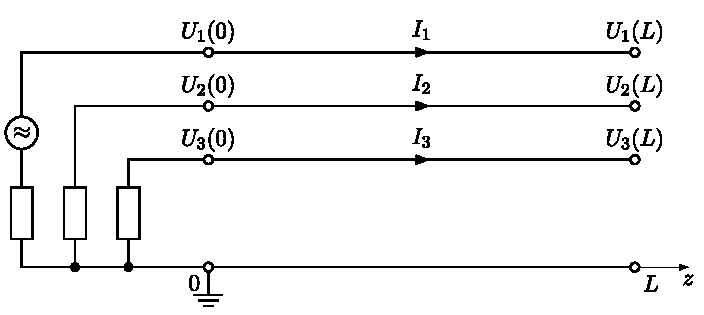
\includegraphics{res/LT7}
\end{center}

Für ein allgemeines $n$-Leitersystem formulieren sich die Telegraphengleichungen \ref{ersttel} und \ref{zweittel} in der verallgemeinerten Matrixform

\begin{equation}\label{verallgmatr}
	\frac{\mathrm{d}}{\mathrm{d} z}\left(\begin{array}{c}
		U_{1}  \\
		U_{2} \\
		\vdots \\
		U_{n}
	\end{array}\right)+\mathbf{Z}^{\prime}\left(\begin{array}{c}
		I_{1} \\
		I_{2} \\
		\vdots \\
		I_{n}
	\end{array}\right)=\left(\begin{array}{c}
		0 \\
		0 \\
		\vdots \\
		0
	\end{array}\right) \quad \frac{\mathrm{d}}{\mathrm{d} z}\left(\begin{array}{c}
		I_{1} \\
		I_{2} \\
		\vdots \\
		I_{n}
	\end{array}\right)+\mathbf{Y}^{\prime}\left(\begin{array}{c}
		U_{1} \\
		U_{2} \\
		\vdots \\
		U_{n}
	\end{array}\right)=\left(\begin{array}{c}
		0 \\
		0 \\
		\vdots \\
		0
	\end{array}\right)
\end{equation}

mit den $n$-Spaltenvektoren $\vec{U}$ und $\vec{I}$ der Leiterspannungen bzw. Leiterströme. Zudem bezeichnen darin $\mathbf{Z}^{\prime}=\mathbf{R}^{\prime}+\mathrm{j} \omega \mathbf{L}^{\prime}$ die $n \times n$ Impedanzmatrix und $\mathbf{Y}^{\prime}=\mathbf{G}^{\prime}+\mathrm{j} \omega \mathbf{C}^{\prime}$ die $n \times n$ Admittanzmatrix. Sie repräsentieren die Resistivitäten, Konduktivitäten, Induktivitäten und Kapazitäten der Einzelleiter sowie der Leitungen untereinander und bilden somit die wechselseitige Beeinflussung innerhalb des Leitersystems ab. Die Impedanzmatrix besitzt die Gestalt

\begin{equation}
	\mathbf{Z}^{\prime}=\left(\begin{array}{cccc}
		R_{1}^{\prime}+R_{\mathrm{G} 11}^{\prime} & R_{\mathrm{G} 12}^{\prime} & \cdots & R_{\mathrm{G} 1 n}^{\prime}  \\
		R_{\mathrm{G} 21}^{\prime} & R_{2}^{\prime}+R_{\mathrm{G} 22}^{\prime} & \cdots & R_{\mathrm{G} 2 n}^{\prime} \\
		\vdots & \vdots & \ddots & \vdots \\
		R_{\mathrm{G} n 1}^{\prime} & R_{\mathrm{G} n 2}^{\prime} & \cdots & R_{n}^{\prime}+R_{\mathrm{G} n n}^{\prime}
	\end{array}\right)+\mathrm{j} \omega\left(\begin{array}{cccc}
		L_{11}^{\prime} & M_{12}^{\prime} & \cdots & M_{1 n}^{\prime} \\
		M_{21}^{\prime} & L_{22}^{\prime} & \cdots & M_{2 n}^{\prime} \\
		\vdots & \vdots & \ddots & \vdots \\
		M_{n 1}^{\prime} & M_{n 2}^{\prime} & \cdots & L_{n n}^{\prime}
	\end{array}\right)
\end{equation}

und enthält die Widerstandsbeläge $R_{i}^{\prime}$ und Selbstinduktivitätsbeläge $L_{i i}^{\prime}$ eines jeden Einzelleiters $i$ sowie die Widerstandbeläge $R_{\mathrm{G} i j}^{\prime}$ des gemeinsamen Rückleiters und Gegeninduktivitätsbeläge\\
$M_{i j}^{\prime}$ zwischen den Leitern $i$ und $j$. Ähnlich verhält es sich mit der Admittanzmatrix

\begin{equation}
	\mathbf{Y}^{\prime}=\left(\begin{array}{cccc}
		G_{11}^{\prime} & G_{12}^{\prime} & \cdots & G_{1 n}^{\prime}  \\
		G_{21}^{\prime} & G_{22}^{\prime} & \cdots & G_{2 n}^{\prime} \\
		\vdots & \vdots & \ddots & \vdots \\
		G_{n 1}^{\prime} & G_{n 2}^{\prime} & \cdots & G_{n n}^{\prime}
	\end{array}\right)+\mathrm{j} \omega\left(\begin{array}{cccc}
		C_{11}^{\prime} & -C_{12}^{\prime} & \cdots & -C_{1 n}^{\prime} \\
		-C_{21}^{\prime} & C_{22}^{\prime} & \cdots & -C_{2 n}^{\prime} \\
		\vdots & \vdots & \ddots & \vdots \\
		-C_{n 1}^{\prime} & -C_{n 2}^{\prime} & \cdots & C_{n n}^{\prime}
	\end{array}\right)
\end{equation}

deren Elemente aus den Leitwertbelägen $G_{i j}^{\prime}$ und Koppelkapazitätsbelägen $C_{i j}^{\prime}$ zwischen den Leitern $i$ und $j$ gebildet werden.

Obiges Differentialgleichungssystem lässt sich aufgrund der Tatsache, dass die Systemmatrizen jeweils voll besetzt sind, nicht auf herkömmlichem Wege mit einem Exponentialansatz oder einer Variation der Konstanten lösen. Man nutzt hierzu stattdessen die sogenannte modale Analyse, die im Folgenden näher erläutert wird.

\subsection{Lösung mittels modaler Analyse}
Aus den beiden Differentialgleichungssystemen erster Ordnung bildet man durch erneutes Ableiten und ineinander Einsetzen zunächst ein System zweiter Ordnung. Für die Leiterspannungen folgt somit


\begin{equation}\label{loesmodan}
	\frac{\mathrm{d}^{2} \vec{U}(z)}{\mathrm{d} z^{2}}-\mathbf{Z}^{\prime} \mathbf{Y}^{\prime} \vec{U}(z)=\overrightarrow{0} 
\end{equation}


Durch eine geeignete und im Weiteren noch zu bestimmende Transformationsmatrix $\mathbf{T}$ soll nun eine Entkopplung der Einzelgleichungen erreicht werden. Mit dieser transformiert sich der Vektor $\vec{U}$ der Leiterspannungen gemäß $\vec{u}=\mathbf{T} \vec{U}$ zu einem modalen Spannungsvektor $\vec{u}$. Umgekehrt erhält man aus dieser rein mathematischen Größe mit der Rücktransformation $\vec{U}=\mathbf{T}^{-1} \vec{u}$ wieder die physikalischen Spannungen der Anordnung. Multiplikation des Differentialgleichungssystems \ref{loesmodan} mit der Matrix $\mathbf{T}$ und Ersetzen des Vektors $\vec{U}$ führt auf das äquivalente System


\begin{align}
	& \frac{\mathrm{d}^{2}}{\mathrm{~d} z^{2}}(\mathbf{T} \vec{U})-\mathbf{T Z} \mathbf{Z}^{\prime} \mathbf{Y}^{\prime}\left(\mathbf{T}^{-1} \vec{u}\right)=\overrightarrow{0}  \\
	& \frac{\mathrm{d}^{2} \vec{u}}{\mathrm{~d} z^{2}}-\underbrace{\mathbf{T Z} \mathbf{Y}^{\prime} \mathbf{T}^{-1}}_{=: \mathbf{D}^{2}} \vec{u}=\overrightarrow{0} 
\end{align}


wobei $\mathbf{D}^{2}$ eine Diagonalmatrix mit den Quadraten der Ausbreitungsparameter $\ubar{\gamma}_{i}$ der $i=1 \ldots n$ Einzelleiter auf der Hauptdiagonale ist. Es gilt

\begin{equation}
	\mathbf{D}^{2}=\mathbf{T Z}^{\prime} \mathbf{Y}^{\prime} \mathbf{T}^{-1}=\left(\begin{array}{cccc}
		\ubar{\gamma}_{1}^{2} & 0 & \cdots & 0  \\
		0 & \ubar{\gamma}_{2}^{2} & \cdots & 0 \\
		\vdots & \vdots & \ddots & \vdots \\
		0 & 0 & \cdots & \ubar{\gamma}_{n}^{2}
	\end{array}\right)=\operatorname{diag}\left(\ubar{\gamma}_{1}^{2}, \ldots, \ubar{\gamma}_{n}^{2}\right)
\end{equation}

Die diagonalisierte Matrixgleichung gestattet es, jeden Einzelleiter separat zu behandeln, da ihre Gleichungen nun nicht mehr miteinander verkoppelt sind. Es lassen sich somit in Analogie zur Einzelleiteranordnung ($\nearrow$\ref{loesULT}) Lösungen der Form


\begin{align}
	\vec{u}(z) & =\mathbf{E}^{+} \vec{u}^{-}+\mathbf{E}^{-} \vec{u}^{+} \label{LTloesform} \\
	\mathbf{T}^{-1} \vec{u}(z)=\vec{U}(z) & =\mathbf{T}^{-1}\left(\mathbf{E}^{+} \mathbf{T} \vec{U}^{-}+\mathbf{E}^{-} \mathbf{T} \vec{U}^{+}\right) 
\end{align}


als Überlagerung von $n$ in positiver bzw. negativer $z$-Richtung propagierenden Spannungsmoden ansetzen, welche im Allgemeinen jeweils unterschiedliche Ausbreitungsgeschwindigkeiten aufweisen. Die Konstantenvektoren $\vec{u}^{ \pm}$bzw. $\vec{U}^{ \pm}$beinhalten dabei die Amplituden der jeweiligen Moden, welche aus entsprechenden Randbedingungen bestimmt werden müssen. Bei der Propagationsmatrix $\mathbf{E}^{ \pm}$handelt es sich um eine Diagonalmatrix der Gestalt

\begin{equation}
	\mathbf{E}^{ \pm}=\left(\begin{array}{cccc}
		\mathrm{e}^{\mp \ubar{\gamma}_{1} z} & 0 & \cdots & 0  \\
		0 & \mathrm{e}^{\mp \ubar{\gamma}_{2} z} & \cdots & 0 \\
		\vdots & \vdots & \ddots & \vdots \\
		0 & 0 & \cdots & \mathrm{e}^{\mp \ubar{\gamma}_{n} z}
	\end{array}\right)=\operatorname{diag}\left(\mathrm{e}^{\mp \ubar{\gamma}_{1} z}, \ldots, \mathrm{e}^{\mp \ubar{\gamma}_{n} z}\right)=\mathrm{e}^{\mp \mathbf{D} z}
\end{equation}

die auf ihrer Hauptdiagonale Exponentialterme enthält, welche die Ausbreitung der einzelnen Moden innerhalb des Leitersystems beschreiben. Ähnlich den Leiterspannungen existieren gleichfalls modale Leiterströme $\vec{i}$, welche man unter Nutzung der Transformationsmatrix $\mathbf{V}$ in äquivalenter Weise aus den physikalischen Strömen $\vec{I}$ gewinnt. Das zugehörige modale Differentialgleichungssystem hierfür lautet


\begin{equation}
	\frac{\mathrm{d}^{2} \vec{i}(z)}{\mathrm{d} z^{2}}-\underbrace{\mathbf{V} \mathbf{Y}^{\prime} \mathbf{Z}^{\prime} \mathbf{V}^{-1}}_{=: \mathbf{D}^{2}} \vec{i}(z)=\overrightarrow{0} 
\end{equation}


und dessen Lösungen lassen sich über die charakteristische modale Impedanzmatrix $\mathbf{z}_{\mathrm{c}}$ bzw. die charakteristische Admittanzmatrix $\mathbf{Y}_{\mathrm{c}}$ gemäß


\begin{align}
	\vec{i}(z) & =\mathbf{z}_{\mathrm{c}}^{-1}\left(\mathbf{E}^{+} \vec{u}^{-}-\mathbf{E}^{-} \vec{u}^{+}\right) \label{loesiform} \\
	\mathbf{V}^{-1} \vec{i}=\vec{I}(z) & =\underbrace{\mathbf{V}^{-1} \mathbf{z}^{-1} \mathbf{T}}_{=: \mathbf{Y}_{\mathrm{c}}} \mathbf{T}^{-1}\left(\mathbf{E}^{+} \mathbf{T} \vec{U}^{-}-\mathbf{E}^{-} \mathbf{T} \vec{U}^{+}\right) \label{loesiform2}
\end{align}


mit den korrespondierenden modalen Spannungen verknüpfen (vergleiche hierzu \ref{loesILT}). Zu jenen Beziehungen gelangt man, indem die erste Telegraphengleichung \ref{verallgmatr} durch linksseitige Multiplikation mit der Matrix $\mathbf{T}$ und unter Anwendung der obigen Transformationsrelationen für die modalen Größen zu


\begin{equation}
	\frac{\mathrm{d} \vec{u}(z)}{\mathrm{d} z}+\mathbf{T Z}^{\prime} \mathbf{V}^{-1} \vec{i}(z)=\overrightarrow{0} 
\end{equation}


umgeformt wird. Einsetzen der Lösung \ref{LTloesform} für die modale Spannung $\vec{u}(z)$ liefert dann


\begin{align}
	-\mathbf{D}\left(\mathbf{E}^{+} \vec{u}^{-}-\mathbf{E}^{-} \vec{u}^{+}\right)+\mathbf{T} \mathbf{T Z}^{\prime} \mathbf{V}^{-1} \vec{i}(z) & =\overrightarrow{0} \quad \mid-\mathbf{D}^{-1} \cdot(\ldots)  \\
	\underbrace{\mathbf{D}^{-1} \mathbf{D}}_{=1}\left(\mathbf{E}^{+} \vec{u}^{-}-\mathbf{E}^{-} \vec{u}^{+}\right)-\underbrace{\mathbf{D}^{-1} \mathbf{T} \mathbf{Z}^{\prime} \mathbf{V}^{-1}}_{=: \mathbf{z}_{c}} \vec{i}(z) & =\overrightarrow{0} 
\end{align}


Umstellen nach dem modalen Leiterstromvektor und Rücktransformation durch linksseitige Multiplikation mit der Matrix $\mathbf{V}^{-1}$ führt schließlich auf die obigen Ausdrücke \ref{loesiform} und \ref{loesiform2}. Die charakteristische Impedanzmatrix $\mathbf{Z}_{c}$ ergibt sich dann aus der inversen Admittanzmatrix unter Anwendung der Regel $(\mathbf{A B})^{-1}=\mathbf{B}^{-1} \mathbf{A}^{-1}$ zur Invertierung des Produktes zweier Matrizen. Es gilt


\begin{align}
	\mathbf{Z}_{c}=\mathbf{Y}_{c}^{-1} & =\left(\mathbf{V}^{-1} \mathbf{z}_{c}^{-1} \mathbf{T}\right)^{-1}=\mathbf{T}^{-1}\left(\mathbf{V}^{-1} \mathbf{z}_{c}^{-1}\right)^{-1}=\mathbf{T}^{-1} \mathbf{z}_{c} \mathbf{V}  \\
	& =\mathbf{T}^{-1}(\mathbf{D}^{-1} \mathbf{T} \mathbf{Z}^{\prime} \underbrace{\left.\mathbf{V}^{-1}\right) \mathbf{V}}_{=1}=\mathbf{T}^{-1} \mathbf{D}^{-1} \mathbf{T} \mathbf{Z}^{\prime} 
\end{align}


Wie werden nun die zur Diagonalisierung genutzten Transformationsmatrizen $\mathbf{T}$ und $\mathbf{V}$ konkret bestimmt? Man betrachte hierzu die Gleichung


\begin{equation}
	\operatorname{det}\left(\mathbf{Z}^{\prime} \mathbf{Y}^{\prime}-\mathbf{D}\right)=\operatorname{det}\left(\mathbf{Z}^{\prime} \mathbf{Y}^{\prime}-\lambda \mathbb{1}\right)=0 
\end{equation}


zur Berechnung der Eigenwerte $\lambda_{i}=\ubar{\gamma}_{i}^{2}$ für das System aus $i=1, \ldots, n$ Leitern. Aus den zugehörigen Eigenvektoren $\vec{t}_{i}$ lässt sich dann die Transformationsmatrix $\mathbf{T}$ gemäß


\begin{equation}
	\left(\mathbf{Z}^{\prime} \mathbf{Y}^{\prime}-\lambda_{i} \mathbb{1}\right) \vec{t}_{i}=\overrightarrow{0} \quad \rightarrow \quad \mathbf{T}=\left(\vec{t}_{i}\right) 
\end{equation}


bilden. Analog verfährt man zur Bestimmung der Matrix $\mathbf{V}$ im Falle der Leiterströme.

Bemerkung 2.1 (Transformationsmatrix für die Lösung des Leiterstromes)

Die Transformationsmatrix $\mathbf{V}$ der Leiterströme $\vec{I}$ unterscheidet sich prinzipiell von der Matrix T zur Transformation der Spannungen $\vec{U}$, da die Matrixmultiplikation nicht kommutativ ist $\left(\mathbf{Y}^{\prime} \mathbf{Z}^{\prime} \neq \mathbf{Z}^{\prime} \mathbf{Y}^{\prime}\right)$ und sich bei deren Bestimmung dementsprechend andere Eigenwerte bzw. Eigenvektoren ergeben. Man kann also nicht wie bei der Einfachleitung die Lösung des Stromes direkt aus der Lösung für die Spannung ableiten.

\subsection{Bestimmung der Impedanz- und Admittanzmatrizen}
\subsubsection{Induktivitätsbestimmung}
Messtechnische Bestimmung: Alle Leiter werden an ihrem Ende gegen Masse kurzgeschlossen. Einer der Leiter (der $j$-te Leiter) wird über eine harmonische Spannungsquelle mit $U_{j}$ angeregt, während alle anderen Leitereingänge offen bleiben. Mit einem Spannungsmesser wird dann die induktive Kopplung zu einem der übrigen Leiter $i$ bestimmt:

\begin{center}
	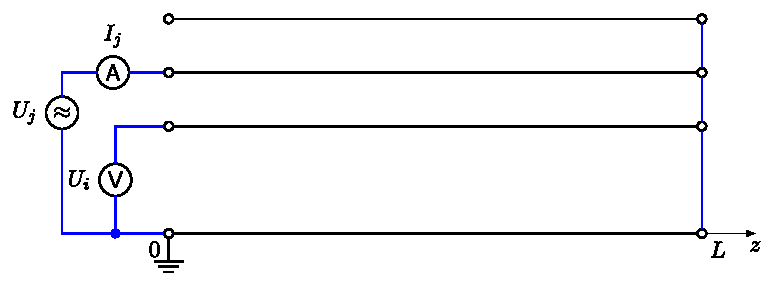
\includegraphics{res/LT8}
\end{center}

Der konkrete Zusammenhang zwischen Spannung und Strom des Messleiters folgt aus \ref{verallgmatr} und wird durch die Gleichung


\begin{equation}
	-\frac{\mathrm{d} U_{i}}{\mathrm{~d} z}=Z_{i 1}^{\prime} I_{1}+Z_{i 2}^{\prime} I_{2}+Z_{i 3}^{\prime} I_{3}+\ldots+Z_{i n}^{\prime} I_{n} 
\end{equation}


beschrieben. Sofern die betrachtete Wellenlänge $\lambda$ sehr viel größer als die Leitungslänge $L$ ist (bei Hochspannungs-Überlandleitungen ist dies zum Beispiel der Fall), kann mit der statischen Näherung $\mathrm{d} z \approx L$ ein Übergang vom Differentialquotienten zum Differenzenquotienten


\begin{equation}
	-\frac{U_{i}(L)-U_{i}(0)}{L}=Z_{i 1}^{\prime} I_{1}+Z_{i 2}^{\prime} I_{2}+Z_{i 3}^{\prime} I_{3}+\ldots+Z_{i n}^{\prime} I_{n} 
\end{equation}


erfolgen. Aufgrund des Kurzschlusses am Leiterende ist nun $U_{i}(L)=0$. Gleichsam fließt in den Leitern mit offenem Eingang bzw. in dem mit einem hochohmigen Spannungsmesser beschalteten Leiter $i$ keinerlei Strom und es ist $I_{k}=0$ für alle $k \neq j$. Damit erhält man schließlich die Relation


\begin{equation}
	U_{i}(0)=Z_{i j}^{\prime} I_{j} L=\mathrm{j} \omega L_{i j}^{\prime} I_{j} L 
\end{equation}


und der Induktivitätsbelag lässt sich durch


\begin{equation}
	L_{i j}^{\prime}=\frac{U_{i}(0)}{j \omega I_{j} L} 
\end{equation}


berechnen. Da die Matrix wegen $L_{i j}^{\prime}=L_{j i}^{\prime}$ eine symmetrische Gestalt hat, müssen insgesamt lediglich $\sum_{k=1}^{n}=\frac{n}{2}(n+1)$ Elemente bestimmt werden.

Analytische Bestimmung: Für eine analytische Berechnung von Gegen- und Selbstinduktivität bedient man sich einer auf James Clerk Maxwell zurückgehenden Vorgehensweise, bei welcher der mittlere geometrische Abstand bzw. mittlere geometrische Radius \footnote{geometric mean distance (GMD) bzw. geometric mean radius (GMR)} einer Leiteranordnung genutzt wird. Man betrachte dazu den Querschnitt eines Leitersystems aus zwei Hin- und zwei Rückleitern gemäß der folgenden Grafik, wobei die Größenordnung der Leiterdimensionen und gegenseitigen Abstände als näherungsweise gleich angenommen werde.

\begin{center}
	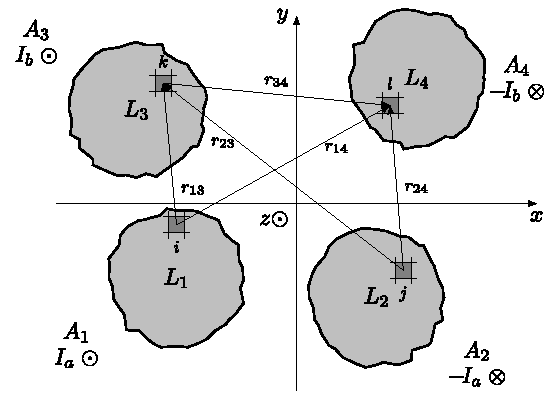
\includegraphics{res/LT9}
\end{center}


Durch die beiden Leiter 1 und 2, welche zusammen den Stromkreis a bilden, fließe der Strom $I_{a}$, durch die Leiter 3 und 4 des Stromkreises b hingegen der Strom $I_{b}$. Dabei werde im Folgenden die Stromverdrängung im Leiter, d.h. der Einfluss von Skin-Effekt und Proximity-Effekt vernachlässigt. Jeder der vier Querschnitte wird nun für die Berechnung in kleine Teilelemente zerlegt. In jedem Leitersegment fließt dann der differentielle Stromanteil


\begin{equation}
	\mathrm{d} I=\vec{J} \mathrm{~d} \vec{A} 
\end{equation}


mit der über der Querschnittsfläche $\vec{A}=A \vec{e}_{z}$ als konstant angenommenen Stromdichte $\vec{J}=J \vec{e}_{z}$. Die einzelnen Segmente der Leiter 1 und 2 tragen demzufolge den Strom


\begin{equation}
	I_{\mathrm{S} 1}=I_{a} \frac{\mathrm{d} A_{1}}{A_{1}} \quad \text { bzw. } \quad I_{\mathrm{S} 2}=-I_{a} \frac{\mathrm{d} A_{2}}{A_{2}} 
\end{equation}


und koppeln damit über das resultierende magnetische Feld in den Stromkreis b ein. Der partielle magnetische Fluss $\mathrm{d} \phi_{k l, i}$ durch die zwischen den Leitersegmenten $k$ und $l$ entlang des Leiterlängenstückes $\mathrm{d} z$ aufgespannten Fläche $A_{34}$, hervorgerufen durch den Strom $\mathrm{d} I_{a}$ im Leitersegment $i$, ist definiert durch


\begin{align}
	\mathrm{d} \phi_{k l, i} & =\iint_{A_{34}} \mathrm{~d} \vec{B} \mathrm{~d} \vec{A}=\mu_{0} \underbrace{\int \mathrm{d} z}_{=\Delta z} \int_{r_{13}}^{r_{14}} \frac{\mathrm{d} I_{a}}{2 \pi r} \mathrm{~d} r=\frac{\mu_{0}}{2 \pi} \Delta z I_{a} \frac{\mathrm{d} A_{1}}{A_{1}} \int_{r_{13}}^{r_{14}} \frac{\mathrm{d} r}{r}  \\
	& =\frac{\mu_{0} \Delta z}{2 \pi} I_{a} \frac{\mathrm{d} A_{1}}{A_{1}}\left(\ln r_{14}-\ln r_{13}\right) 
\end{align}


Der Beitrag des Elementes $j$ des Leiters 2 ergibt sich analog zu


\begin{equation}
	\mathrm{d} \phi_{k l, j}=-\frac{\mu_{0} \Delta z}{2 \pi} I_{a} \frac{\mathrm{d} A_{2}}{A_{2}} \int_{r_{23}}^{r_{24}} \frac{\mathrm{d} r}{r}=-\frac{\mu_{0} \Delta z}{2 \pi} I_{a} \frac{\mathrm{d} A_{2}}{A_{2}}\left(\ln r_{24}-\ln r_{23}\right) 
\end{equation}

Den vollständigen magnetischen Fluss zwischen den Leitersegmenten $k$ und $l$, hervorgerufen durch den Gesamtstrom $I_{a}$ in den Leitern 1 und 2, erhält man nun durch eine Integration über die jeweiligen Leiterffächen $A_{1}$ und $A_{2}$ gemäß


\begin{equation}
	\phi_{k l, a}=\frac{\mu_{0} \Delta z}{2 \pi} I_{a}\left[\frac{1}{A_{1}} \iint_{A_{1}} \ln r_{14} \mathrm{~d} A_{1}-\frac{1}{A_{1}} \iiint_{A_{1}} \ln r_{13} \mathrm{~d} A_{1}-\frac{1}{A_{2}} \iint_{A_{2}} \ln r_{24} \mathrm{~d} A_{2}+\frac{1}{A_{2}} \iint_{A_{2}} \ln r_{23} \mathrm{~d} A_{2}\right] 
\end{equation}


Dieser ist jedoch je nach Lage der Segmente $k$ und $l$ innerhalb der Leiterquerschnitte verschieden, sodass für die Berechnung des vollständigen gekoppelten Flusses zwischen den Leitern 3 und 4 bei der Integration über die Leiterflächen $A_{3}$ und $A_{4}$ der algebraische Mittelwert zu verwenden ist. Letztlich führt dies auf folgende Summe aus doppelten Flächenintegralen

\begin{equation}
	\begin{array}{r}
		\bar{\phi}_{a b}=\frac{\mu_{0} \Delta z}{2 \pi} I_{a}\left[\frac{1}{A_{1} A_{4}} \iint_{A_{4}} \iint_{A_{1}} \ln r_{14} \mathrm{~d} A_{1} \mathrm{~d} A_{4}-\frac{1}{A_{1} A_{3}} \iint_{A_{3}} \iint_{A_{1}} \ln r_{13} \mathrm{~d} A_{1} \mathrm{~d} A_{3}\right. \\
		\left.-\frac{1}{A_{2} A_{4}} \iint_{A_{4}} \iint_{A_{2}} \ln r_{24} \mathrm{~d} A_{2} \mathrm{~d} A_{4}+\frac{1}{A_{2} A_{3}} \iint_{A_{3}} \iint_{A_{2}} \ln r_{23} \mathrm{~d} A_{2} \mathrm{~d} A_{3}\right] 
	\end{array}
\end{equation}

Die längenbezogene Gegeninduktivität zwischen den Leiterstromkreisen a und b infolge des Stromes $I_{a}$ ist dann durch


\begin{equation}\label{leitstromkrei}
	M_{a b}^{\prime}=\frac{\bar{\phi}_{a b}}{I_{a} \Delta z}=\frac{\bar{\phi}_{b a}}{I_{a} \Delta z}=M_{b a}^{\prime} 
\end{equation}


gegeben.

Führt man nun den mittleren geometrischen Abstand $g_{i j}$ ein und definiert diesen über seinen natürlichen Logarithmus gemäß


\begin{equation}
	\ln g_{i j}:=\frac{1}{A_{i} A_{j}} \iint_{A_{i}} \iint_{A_{j}} \ln r_{i j} \mathrm{~d} A_{j} \mathrm{~d} A_{i} 
\end{equation}


mit $r_{i j}$ als dem Abstand zwischen einem Segment $\mathrm{d} A_{i}$ des Leiterquerschnittes $A_{i}$ zu einem Element $\mathrm{d} A_{j}$ der Leiterfläche $A_{j}$, so wird der Ausdruck \ref{leitstromkrei} für die Gegeninduktivität damit schließlich zu


\begin{equation}\label{gengenindschlieszu}
	M_{a b}^{\prime}=\frac{\mu_{0}}{2 \pi}\left(\ln g_{14}-\ln g_{13}-\ln g_{24}+\ln g_{23}\right)=\frac{\mu_{0}}{2 \pi} \ln \left(\frac{g_{14} g_{23}}{g_{13} g_{24}}\right) 
\end{equation}


Im Spezialfall einer lateralen Anordnung der Leiter mit kreisförmigen Leiterquerschnitten und den gegenseitigen Abständen $d_{a}, d_{b}$ und $D$ entsprechend der Grafik:

\begin{center}
	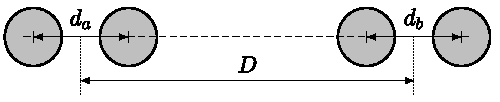
\includegraphics{res/LT10}
\end{center}

sowie unter der Bedingung $d_{a}, d_{b} \ll D$ vereinfachen sich die jeweiligen mittleren geometrischen Abstände zu

\begin{equation}
	\begin{array}{ll}
		g_{14} \approx r_{14}=D+\frac{d_{a}+d_{b}}{2} & g_{23} \approx r_{23}=D-\frac{d_{a}+d_{b}}{2} \\
		g_{13} \approx r_{13}=D+\frac{d_{a}-d_{b}}{2} & g_{24} \approx r_{24}=D-\frac{d_{a}-d_{b}}{2} 
	\end{array}
\end{equation}

Insbesondere in der Energietechnik ist die äquidistante Leiteranordnung mit $d:=d_{a}=d_{b}$ ein häufig anzutreflender praktischer Fall. Hierfür folgt dann entsprechend


\begin{equation}
	g_{14}=D+d \quad, \quad g_{23}=D-d \quad, \quad g_{13}=g_{24}=D 
\end{equation}


was auf einen Gegeninduktivitätsbelag der Übertragungsleitungen von


\begin{equation}
	M_{a b}^{\prime}=\frac{\mu_{0}}{\pi} \ln \left(\frac{\sqrt{D^{2}-d^{2}}}{D}\right) 
\end{equation}


führt. Haben die beiden Stromkreise weiterhin einen gemeinsamen Rückleiter $n$, so stellt sich der Gegeninduktivitätsbelag zwischen den Leiterkreisen $i-n$ und $j-n$ dagegen in der Form


\begin{equation}
	M_{i j}^{\prime}=\frac{\mu_{0}}{2 \pi} \ln \left(\frac{g_{i n} g_{j n}}{g_{i j} g_{n n}}\right) 
\end{equation}


dar, wobei $g_{i n}, g_{j n}$ und $g_{i j}$ die mittleren geometrischen Abständen der Leiter $i$ und $j$ zum Referenzleiter $n$ bzw. der Leiter $i$ und $j$ zueinander bezeichnen. Die Größe $g_{n n}$ ist dagegen der mittlere geometrische Abstand


\begin{equation}
	\ln g_{n n}=\frac{1}{A_{n}^{2}} \iint_{A_{n}} \iint_{A_{n}} \ln r_{n n} \mathrm{~d} A_{n} \mathrm{~d} A_{n} 
\end{equation}


der Querschnittsfläche $A_{n}$ des Neutralleiters zu sich selbst; $r_{n n}$ nimmt während der Integration somit alle möglichen Werte des Abstandes zwischen zwei verschiedenen Leitersegmenten $\mathrm{d} A_{n}$ der Fläche $A_{n}$ an.

Berechnung der Selbstinduktivität Auf analoge Weise erfolgt die Berechnung der Selbstinduktivität, die als der Quotient des Koppelflusses eines Stromkreises infolge des durch ihn hindurchfließenden Stromes und ebenjenen Leiterstromes definiert ist. Hierfür werde der nachfolgend dargestellte zusammengefasste Querschnitt des Vierleitersystems betrachtet, es wurden wurden die Hin- und Rückleiter $L_{1}$ und $L_{3}$ bzw. $L_{2}$ und $L_{4}$ zusammengefasst.

\begin{center}
	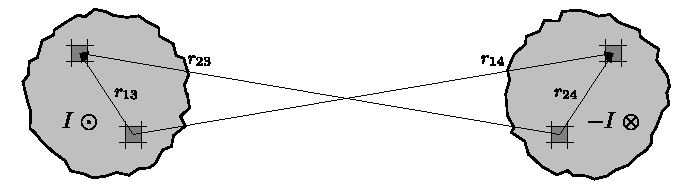
\includegraphics{res/LT11}
\end{center}


Durch die Überlagerung der Stromkreise a und b fallen die Leiterquerschnittsflächen mit $A_{1}=A_{3}$ und $A_{2}=A_{4}$ zusammen und gilt für die Abstände zwischen den Segmenten folglich $r_{14}=r_{23}$, $r_{13}=r_{33}=r_{11}, r_{24}=r_{44}=r_{22}$ und $r_{33}=r_{44}$. Somit folgt für die mittleren geometrischen Abstände unmittelbar $g_{14}=g_{23}$ usw. und der Selbstinduktivitätsbelag bestimmt sich aus dem vorigen Ergebnis in Gleichung \ref{gengenindschlieszu} gemäß


\begin{equation}\label{gleigem}
	M_{a}^{\prime}=\frac{\mu_{0}}{2 \pi} \ln \left(\frac{g_{23}^{2}}{g_{13} g_{24}}\right)=\frac{\mu_{0}}{2 \pi} \ln \left(\frac{g_{23}^{2}}{g_{33} g_{44}}\right) 
\end{equation}


Praktisch kann die Berechnung der Logarithmenterme Probleme bereiten, falls sich das Argument zu Null ergibt und der Wert des Logarithmus demzufolge unbestimmt wird. In diesem Fall muss dann bei der Auswertung der Integrale der Hauptwert gebildet werden.

Verallgemeinert man Gleichung \ref{gleigem} für ein Mehrleitersystem mit einem Neutral- bzw. Rückleiter $n$, so lautet der Ausdruck für den Selbstinduktivitätsbelag des $i$-ten Leiters nun


\begin{equation}
	M_{i i}^{\prime}=\frac{\mu_{0}}{2 \pi} \ln \left(\frac{g_{i n}^{2}}{g_{i i} g_{n n}}\right) 
\end{equation}


Selbst- und Gegeninduktivität von Leitern über einer leitfähigen Ebene Im Falle von Leitersystemen über einer leitfähigen Ebene, wie dies z.B. bei Überlandleitungen zur elektrischen Energieübertragung gegeben ist, werden die involvierten Ströme an der Ebene gespiegelt \footnote{Zur Anwendung des Spiegelungsprinzips sei der Einfachheit halber von einer ideal leitenden Ebene ausgegangen. In der Realität besitzt das Erdreich einer Überlandleitung jedoch stets eine endliche Leitfähigkeit, sodass sich die Berechnung hier etwas komplizierter darstellt.}. Für die Bestimmung der Selbst- und Gegeninduktivitätsbeläge kann dann auf die zuvor erhaltenen Ergebnisse zurückgegriffen werden. Beispielhaft sie hierzu die nachfolgend abgebildete Querschnittsanordnung betrachtet.

\begin{center}
	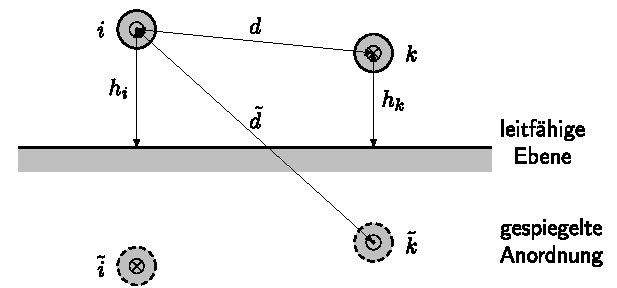
\includegraphics{res/LT12}
\end{center}


Im vorliegenden Fall berechnet sich der Gegeninduktivitätsbelag eines Leiters anhand von Gleichung \ref{gengenindschlieszu} und unter Berücksichtigung der jeweiligen Spiegelströme also gemäß


\begin{equation}
	M_{i k}^{\prime}=\frac{1}{2} \frac{\mu_{0}}{2 \pi} \ln \left(\frac{g_{i \tilde{k}} g_{k \tilde{i}}}{g_{i k} g_{i \tilde{k}}}\right) 
\end{equation}


Der Vorfaktor $\frac{1}{2}$ resultiert dabei aus der Tatsache, dass für die Gegeninduktivität lediglich der tatsächliche Fluss oberhalb der leitfähigen Ebene berücksichtigt werden darf. Zusammen mit den Beziehungen $g_{i \tilde{k}}=\tilde{d}=g_{i k}$ und $g_{i k}=g_{i \tilde{i}}=d$ für die gegenseitigen Abstände der Leiter und ihrer Spiegelbilder ergibt sich demnach


\begin{equation}
	M_{i k}^{\prime}=\frac{\mu_{0}}{4 \pi} \ln \left(\frac{g_{i \tilde{k}}}{g_{i k}}\right)^{2}=\frac{\mu_{0}}{2 \pi} \ln \left(\frac{g_{i \tilde{i}}}{g_{i k}}\right)=\frac{\mu_{0}}{2 \pi} \ln \left(\frac{\tilde{d}}{d}\right) 
\end{equation}


Gleichfalls erhält man für den Selbstinduktivitätsbelag nach Gleichung \ref{gleigem} mit $i=k$ und $g_{i \tilde{i}}=2 h_{i}$ sowie $g_{i i}=g_{i \tilde{i}}=r_{i i}$ den Ausdruck


\begin{equation}
	M_{i i}^{\prime}=\frac{\mu_{0}}{4 \pi} \ln \left(\frac{g_{i \tilde{i}}^{2}}{g_{i i} g_{\tilde{i i}}}\right)=\frac{\mu_{0}}{2 \pi} \ln \left(\frac{2 h_{i}}{r_{i i}}\right) 
\end{equation}

\subsubsection{Kapazitätsbestimmung}
Messtechnische Bestimmung: Einer der Leiter (der $j$-te Leiter) wird über eine Spannungsquelle mit der harmonischen Spannung $U_{j}$ angeregt, während alle übrigen an ihrem Leitungsanfang gegen den Referenzleiter kurzgeschlossen werden. Sämtliche Leiterabschlüsse bleiben hingegen offen. Im Leiter $i$ wird nun der aufgrund der kapazitiven Kopplung hervorgerufene Strom $I_{i}$ mittels eines Amperemeters gemessen:

\begin{center}
	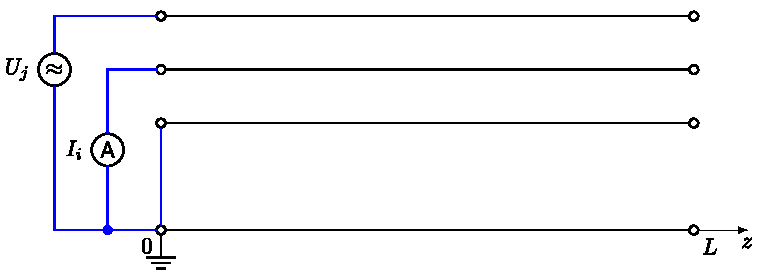
\includegraphics{res/LT13}
\end{center}

Für den gemessenen Leiterstrom lässt sich nach \ref{verallgmatr} die Differentialgleichung


\begin{equation}
	-\frac{\mathrm{d}}{\mathrm{d} z} I_{i}=Y_{i 1}^{\prime} U_{1}+Y_{i 2}^{\prime} U_{2}+Y_{i 3}^{\prime} U_{3}+\ldots+Y_{i n}^{\prime} U_{n} 
\end{equation}


aufstellen. Unter der Bedingung einer im Vergleich zur verwendeten Wellenlänge kurzen Leiterlänge $L \ll \lambda$ (statische Näherung) kann wiederum ein Übergang zum Differenzenquotienten


\begin{equation}
	-\frac{I_{i}(L)-I_{i}(0)}{L}=Y_{i 1}^{\prime} U_{1}+Y_{i 2}^{\prime} U_{2}+Y_{i 3}^{\prime} U_{3}+\ldots+Y_{i n}^{\prime} U_{n} 
\end{equation}


erfolgen. An den kurzgeschlossenen Leitereingängen gilt nun für die Spannung $U_{k}(0)=0$ mit $k \neq j$. Gleichsam sind alle Ströme am offenen Leiterende Null und mit $I_{i}(L)=0$ folgt schließlich die Beziehung


\begin{equation}
	I_{i}(0)=Y_{i j}^{\prime} U_{j} L=\mathrm{j} \omega C_{i j}^{\prime} U_{j} L 
\end{equation}


sodass der Kapazitätsbelag über


\begin{equation}
	C_{i j}^{\prime}=\frac{I_{i}(0)}{j \omega U_{j} L} 
\end{equation}


berechnet werden kann. Problematisch ist in der Praxis die Messungenauigkeit bei niedrigen Frequenzen und den hierbei geringen Strömen, wodurch der Ausdruck für $C_{i j}^{\prime}$ unbestimmt wird. Gleichfalls ist die Anwendbarkeit der Messmethode auch zu hohen Frequenzen hin limitiert, wenn die Leiterlänge nicht mehr als klein im Verhältnis zur Wellenlänge angenommen werden kann.

Analytische Bestimmung: Die Kapazität ist allgemein als das Verhältnis von Ladungsmenge $Q$ zur Spannung $U$ definiert. Die Ladung eines Quellgebietes der Raumladungsdichte $\rho_{\mathrm{V}}$ bestimmt man über das GaUsSsche Gesetz der MAXWELL-Gleichungen gemäß


\begin{equation}
	\varepsilon \iiint_{V} \div \vec{E} \mathrm{~d} V=\varepsilon \oiint_{\partial V} \vec{E} \mathrm{~d} \vec{A}=\iiint_{V} \rho_{\mathrm{V}} \mathrm{d} V=Q 
\end{equation}


während sich die Spannung nach Definition des elektrischen Skalarpotentials $\phi$ aus der Berechnung des Wegintegrals


\begin{equation}
	U=\Delta \phi=\int \vec{E} \mathrm{~d} \vec{r} 
\end{equation}


ergibt. Für die Kapazität $C$ folgt demnach mit dem Ladungsbelag $q^{\prime}=\frac{Q}{\Delta z}$ die Beziehung


\begin{equation}
	C=\frac{Q}{U}=\frac{q^{\prime} \Delta z}{U}=\varepsilon_{0} \varepsilon_{\mathrm{r}} \frac{\oiint \vec{E} \mathrm{~d} \vec{A}}{\int \vec{E} \mathrm{~d} \vec{r}} 
\end{equation}


Hierfür muss folglich das elektrische Feld $\vec{E}$ der Anordnung bekannt sein. Für ausgewählte Leitergeometrien mit einem oder zwei Leitern sind explizite analytische Lösungen möglich. Beispielhaft sei die Berechnung der Kapazitätsbeläge für das nachfolgend dargestellte Dreileitersystem über einer leitfähigen Ebene als gemeinsamer Referenzleiter mit den partiellen Kapazitäten $\bar{C}$ der Einzelleiter untereinander sowie gegenüber der Ebene erläutert.

\begin{center}
	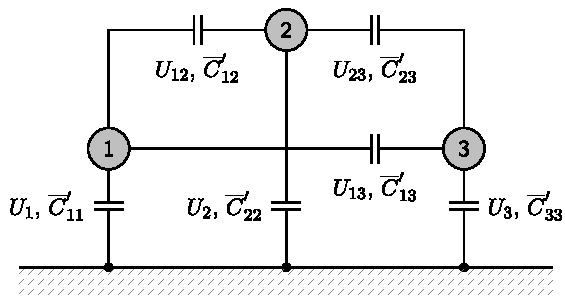
\includegraphics{res/LT14}
\end{center}

Die Potentialdifferenzen bzw. Spannungen zwischen den Leitern sind dabei mit $U_{12}, U_{13}$ und $U_{23}$ bezeichnet, während die Leiterspannungen gegenüber dem Referenzleiter als $U_{1}, U_{2}$ und $U_{3}$ angegeben sind. Konkret setzen sich die Ladungsbeläge $q^{\prime}$ der drei Leiter wie folgt zusammen


\begin{align}
	q_{1}^{\prime} & =\bar{C}_{11}^{\prime} U_{1}+\bar{C}_{12}^{\prime} U_{12}+\bar{C}_{13}^{\prime} U_{13}=\bar{C}_{11}^{\prime} U_{1}+\bar{C}_{12}^{\prime}\left(U_{1}-U_{2}\right)+\bar{C}_{13}^{\prime}\left(U_{1}-U_{3}\right)  \\
	& =\left(\bar{C}_{11}^{\prime}+\bar{C}_{12}^{\prime}+\bar{C}_{13}^{\prime}\right) U_{1}-\bar{C}_{12}^{\prime} U_{2}-\bar{C}_{13}^{\prime} U_{3}  \\
	q_{2}^{\prime} & =-\bar{C}_{21}^{\prime} U_{1}+\left(\bar{C}_{21}^{\prime}+\bar{C}_{22}^{\prime}+\bar{C}_{23}^{\prime}\right) U_{2}-\bar{C}_{23}^{\prime} U_{3}  \\
	q_{3}^{\prime} & =-\bar{C}_{31}^{\prime} U_{1}-\bar{C}_{32}^{\prime} U_{2}+\left(\bar{C}_{31}^{\prime}+\bar{C}_{32}^{\prime}+\bar{C}_{33}^{\prime}\right) U_{3} 
\end{align}


Werden die statischen Kapazitätsbeläge $C^{\prime}$ über


\begin{equation}
	C_{i i}^{\prime}=\sum_{j=1}^{n} \bar{C}_{i j}^{\prime} \quad \text { und } \quad C_{i j}^{\prime}=-\bar{C}_{i j}^{\prime} 
\end{equation}


durch die partiellen Kapazitätsbeläge $\bar{C}^{\prime}$ ausgedrückt, erhält man hiermit die Matrixgleichung

\begin{equation}
	\left(\begin{array}{c}
		q_{1}^{\prime}  \\
		q_{2}^{\prime} \\
		\vdots \\
		q_{n}^{\prime}
	\end{array}\right)=\underbrace{\left(\begin{array}{cccc}
			C_{11}^{\prime} & C_{12}^{\prime} & \cdots & C_{1 n}^{\prime} \\
			C_{21}^{\prime} & C_{22}^{\prime} & \cdots & C_{2 n}^{\prime} \\
			\vdots & \vdots & \ddots & \vdots \\
			C_{n 1}^{\prime} & C_{n 2}^{\prime} & \cdots & C_{n n}^{\prime}
		\end{array}\right)}_{=: \mathrm{C}^{\prime}}\left(\begin{array}{c}
		U_{1} \\
		U_{2} \\
		\vdots \\
		U_{n}
	\end{array}\right)
\end{equation}

mit der statischen bzw. MAXwELLschen Kapazitätsmatrix $\mathbf{C}^{\prime}$.

Berechnung der statischen Kapazitäten Um die Elemente der statischen Kapazitätsmatrix $\mathbf{C}^{\prime}$ bestimmen zu können, müssen die einzelnen Ladungsbeläge und Potentiale auf den Leitern bekannt sein. Während sich die Spannung in der Regel ohne Probleme messen lässt, sind Ladungen dagegen nur sehr schwer direkt ermittelbar. Man erhält diese daher häufig aus analytischen oder numerischen Rechnungen.

Im Gegensatz zur Berechnung der Koppelinduktivitäten hängen die Kapazitäten allerdings von der vollständigen Geometrie aller Leiter des Systems ab. Man behilft sich daher mit der Definition der sogenannten Potentialkoeffizientenmatrix $\mathbf{K}^{\prime}$ gemäß


\begin{equation}
	\vec{U}=\mathbf{K}^{\prime} \vec{q}^{\prime} \quad \text { mit } \quad \mathbf{C}^{\prime}=\mathbf{K}^{\prime-1} 
\end{equation}


sodass die statischen Kapazitätsmatrix hieraus durch Invertieren berechnet werden kann. Die Potentialkoeffizienten gestatten dabei eine analytische Behandlung im Falle einiger spezieller Leiteranordnungen. So folgt zum Beispiel aus dem elektrischen Feld


\begin{equation}
	\vec{E}(\vec{r})=\iiint_{V} \rho_{\mathrm{V}}\left(\vec{r}^{\prime}\right) \frac{\vec{r}-\vec{r}^{\prime}}{\left|\vec{r}-\vec{r}^{\prime}\right|^{3}} \mathrm{~d} V 
\end{equation}


für den Spezialfall zylindrischer Leiter in einem homogenen Medium über einer leitfähigen Ebene (Hochspannungs-Übertragungsleitungen) mittels Spiegelungsmethode die Beziehung


\begin{equation}
	K_{i j}^{\prime}=\frac{1}{2 \pi \varepsilon_{0}} \ln \left(\frac{r_{i \tilde{j}}}{r_{i j}}\right) \quad, \quad\left[K^{\prime}\right]=1 \mathrm{~m} / \mathrm{F} 
\end{equation}


mit $r_{i j}$ und $r_{i \tilde{j}}$ als dem Abstand des Leiters $i$ zum Leiter $j$ bzw. zu dessen Spiegelbild $\tilde{j}$.

\subsection{Baum-Liu-Tesche-Gleichung für Mehrfachleitungen}
\subsubsection{Netzwerke}
Um ein Leitungssystem als elektrisches Netzwerk zu modellieren, müssen die wesentlichen Ausbreitungswege elektromagnetischer Wellen (ausgedehnte Leitungen, Gehäuseschirme etc.) sowie die möglichen Streuzentren innerhalb des Systems (Leitungsknicke, Verzweigungen usw.) identifiziert werden. Eine derartige Netzwerktopologie besteht dabei aus

\begin{itemize}
	\item den Kanten, welche die vorhandenen Propagationswege - ausgedrückt durch Propagationsmatrizen - beschreiben, sowie
	\item den Knoten bzw. Ecken, welche den Streuzentren - dargestellt durch ihre Streumatrizen entsprechen.
\end{itemize}

Das vollständige elektrische Netzwerk wird dann mithilfe der BLT-Gleichung gelöst. Die Nummerierung der einzelnen Netzwerkelemente bestimmt die Gestalt der Knotenmatrix. 

\subsubsection{Knotenmatrix}
Betrachtet wird nun die Streumatrix eines Knotens $\nu$ mit den Kanten $\mu$. Für die einfallenden und reflektierten Wellen gilt die Beziehung


\begin{equation}
	\left(\left(U^{\mathrm{refl}}\right)_{\mu}\right)_{\nu}=\left((S)_{\mu, \mu^{\prime}}\right)_{\nu} \cdot\left(\left(U^{\mathrm{inc}}\right)_{\mu}\right)_{\nu} 
\end{equation}


mit den Vektoren der reflektierten und inzidenten Wellenspannungen


\begin{equation}
	\vec{U}^{\mathrm{refl}}=\vec{a} \sqrt{\mathbf{Z}_{\mathrm{C}}} \quad \text { bzw. } \quad \overrightarrow{U^{\mathrm{inc}}}=\vec{b} \sqrt{\mathbf{Z}_{\mathrm{C}}} 
\end{equation}


eines Knotens, welche über die Matrix der Leitungswellenimpedanzen $\mathbf{Z}_{C}$ in Beziehung gesetzt werden. Diese Spannungsvektoren sind dabei sogenannte Mehrebenenvektoren. Beispielsweise sei

\begin{equation}
	\vec{x}=\left(\begin{array}{l}
		x_{1}  \\
		x_{2} \\
		x_{3} \\
		x_{4} \\
		x_{5}
	\end{array}\right) \in \mathbb{K}^{5}
\end{equation}

mit den Elementen $x_{1}, x_{2}$ eines Zweileitersystems und den Elementen $x_{3}, x_{4}, x_{5}$ eines Dreileitersystems. Mithilfe der freien Summe $\dot{+}$ lässt sich dies umschreiben zu

\begin{equation}
	\vec{x}=\begin{pmatrix}\begin{pmatrix}{x_{1}}\\{x_{2}}\end{pmatrix}\\\begin{pmatrix}
			x_{3}  \\
			x_{4} \\
			x_{5}
	\end{pmatrix}\end{pmatrix}=\underbrace{\binom{x_{1}}{x_{2}}}_{\in \mathbb{K}^{2}}\dot{+}\underbrace{\left(\begin{array}{l}
			x_{3} \\
			x_{4} \\
			x_{5}
		\end{array}\right)}_{\in \mathbb{K}^{3}}
\end{equation}

womit für den Spannungsvektor der reflektierten Welle folgt

\begin{equation}
	\left(\left(U^{\mathrm{refl}}\right)_{\mu}\right)_{\nu}=\left(\left(\begin{array}{c}
		U_{1,1}^{\mathrm{refl}}  \\
		U_{1,2}^{\mathrm{refl}} \\
		\vdots \\
		U_{1, n_{1}}^{\mathrm{refl}}
	\end{array}\right)_{1}\left(\begin{array}{c}
		U_{2,1}^{\mathrm{refl}} \\
		U_{2,2}^{\mathrm{refl}} \\
		\vdots \\
		U_{2, n_{2}}^{\mathrm{refl}}
	\end{array}\right)_{2} \ldots .\left(\begin{array}{c}
		U_{\mu, 1}^{\mathrm{refl}} \\
		U_{\mu, 2}^{\mathrm{ref}} \\
		\vdots \\
		U_{\mu, n_{\mu}}^{\mathrm{refl}}
	\end{array}\right)_{\mu}\right)_{\nu}
\end{equation}

Die Streumatrix besitzt dann die Dimension


\begin{equation}
	\operatorname{dim}\left((S)_{\mu, \mu^{\prime}}\right)_{\nu}=N_{\nu} \times N_{\nu^{\prime}} \quad \text { mit } \quad N_{\nu}=\sum_{i=1}^{\mu} n_{i} 
\end{equation}


Die Bestimmung von $U^{\text {refl }}$ und $U^{\text {inc }}$ erfolgt über


\begin{align}
	\left(\left(U^{\mathrm{refl}}\right)_{\mu}\right)_{\nu} & :=\left(\left(U_{1}\right)_{\mu}\right)_{\nu}+\left(\left(Z_{\mathrm{C}}\right)_{\mu, \mu^{\prime}}\right)_{\nu}\left(\left(I_{1}\right)_{\mu}\right)_{\nu}  \\
	\left(\left(U^{\mathrm{inc}}\right)_{\mu}\right)_{\nu} & :=\left(\left(U_{1}\right)_{\mu}\right)_{\nu}-\left(\left(Z_{\mathrm{C}}\right)_{\mu, \mu^{\prime}}\right)_{\nu}\left(\left(I_{1}\right)_{\mu}\right)_{\nu} 
\end{align}


mit der Gesamtspannung $\vec{U}_{1}$ am Eingang der Leitung und dem Gesamtstrom $\vec{I}_{1}$. Es ist darin


\begin{align}
	&\left(\left(U_{1}\right)_{\mu}\right)_{\nu}=\frac{1}{2}\left[\left(\left(U^{\mathrm{refl}}\right)_{\mu}\right)_{\nu}+\left(\left(U^{\mathrm{inc}}\right)_{\mu}\right)_{\nu}\right]  \\
	&\left(\left(I_{1}\right)_{\mu}\right)_{\nu}=\frac{1}{2}\left(\left(Z_{\mathrm{C}}\right)_{\mu, \mu^{\prime}}\right)_{\nu}\left[\left(\left(U^{\mathrm{refl}}\right)_{\mu}\right)_{\nu}-\left(\left(U^{\mathrm{inc}}\right)_{\mu}\right)_{\nu}\right] 
\end{align}


Einsetzen und Umstellen nach den inzidenten und reflektierten Spannungen führt schließlich auf


\begin{equation}
	\left((S)_{\mu, \mu^{\prime}}\right)_{\nu}=\left[\left((Z)_{\mu, \mu^{\prime}}\right)_{\nu}\left(\left(Z_{\mathrm{C}}\right)_{\mu, \mu^{\prime}}\right)_{\nu}^{-1}-\left((E)_{\mu, \mu^{\prime}}\right)_{\nu}\right]^{-1}\left[\left((Z)_{\mu, \mu^{\prime}}\right)_{\nu}\left(\left(Z_{\mathrm{C}}\right)_{\mu, \mu^{\prime}}\right)_{\nu}^{-1}+\left((E)_{\mu, \mu^{\prime}}\right)_{\nu}\right] 
\end{equation}


mit der Einheitsmatrix $\left((E)_{\mu, \mu^{\prime}}\right)_{\nu}$ am Knoten $\nu$. Für alle Knoten ist eine Streumatrix zu erstellen und nach dem Schema der Welleninzidenzmatrix bzw. Wellenverbindungsmatrix anzuordnen.

\subsubsection{Propagationsmatrix}
Aus der Theorie der Mehrfachleitungen ergibt sich die Spannung $\vec{U}(z)$ als Überlagerung der in positiver und negativer $z$-Richtung laufenden Wellen $\vec{U}^{ \pm}(z)$ gemäß


\begin{equation}
	\vec{U}(z)=\vec{U}^{+}(z)+\vec{U}^{-}(z) 
\end{equation}


Eine Verknüpfung der reflektierten Wellen am Anfang der Leitung mit den inzidenten Wellen führt auf

\begin{equation}
	\underbrace{\binom{\vec{U}^{+}(0)}{\vec{U}^{-}(L)}}_{\begin{array}{c}
			\text { Vektor der }  \\
			\text { refl. Wellen }
	\end{array}}=\left(\begin{array}{cc}
		0 & \mathbf{T}^{-1} \mathrm{e}^{\mathbf{D} L} \mathbf{T} \\
		\mathbf{T}^{-1} \mathrm{e}^{\mathrm{D} L} \mathbf{T} & 0
	\end{array}\right) \cdot \underbrace{\binom{\vec{U}^{-}(0)}{\vec{U}^{+}(L)}}_{\begin{array}{c}
			\text { Vektor der } \\
			\text { inzid. Wellen }
	\end{array}}+\frac{1}{2} \vec{U}_{\mathrm{S}}
\end{equation}

In kompakter Form geschrieben, lautet diese Relation


\begin{equation}
	\left(\vec{U}^{\mathrm{ref}}\right)_{\tau}=\left(\mathbf{P}_{m, n}\right)_{\tau}\left(\vec{U}^{\mathrm{inc}}\right)_{\tau}+\frac{1}{2}\left(\vec{U}_{\mathrm{S}}\right)_{\tau} 
\end{equation}


unter Verwendung der Propagationsmatrix $\left(\mathbf{P}_{m, n}\right)_{\tau}$ entlang einer Kante $\tau$, geordnet nach den Wellen $m$ und $n$.

\subsubsection{Netzwerk-BLT-Gleichung}
Die Streubeziehung zwischen reflektierten und inzidenten Wellen ist durch


\begin{equation}
	\left(U^{\mathrm{refl}}\right)_{i}=\left((S)_{\mu, \mu^{\prime}}\right)_{i, j}\left(U^{\mathrm{inc}}\right)_{i} 
\end{equation}


gegeben, wobei der index $i$ den entsprechenden Eintrag der Netzwerkmatrix bezeichnet. Die Propagation entlang der Kanten wird mithilfe der Gleichung


\begin{equation}
	\left(U^{\mathrm{refl}}\right)_{i}=\left((P)_{\mu, \mu^{\prime}}\right)_{i, j}\left(U^{\mathrm{inc}}\right)_{i}+\frac{1}{2}\left(U_{\mathrm{S}}\right)_{i} 
\end{equation}


beschrieben. Gleichsetzen und Auflösen nach den inzidenten Wellen $\left(U^{\text {inc }}\right)_{i}$ führt auf


\begin{equation}
	\left(U^{\mathrm{inc}}\right)_{i}=\frac{1}{2}\left[\left((S)_{\mu, \mu^{\prime}}\right)_{i, j}-\left((P)_{\mu, \mu^{\prime}}\right)_{i, j}\right]^{-1}\left(U_{\mathrm{S}}\right)_{i} 
\end{equation}


Die Überlagerung von inzidenten und reflektierten Wellen ergibt letztlich


\begin{align}
	(U)_{i} & =\left(U^{\mathrm{inc}}\right)_{i}+\left(U^{\mathrm{refl}}\right)_{i}=\left(U^{\mathrm{inc}}\right)_{i}+\left((S)_{\mu, \mu^{\prime}}\right)_{i, j}\left(U^{\mathrm{ref}}\right)_{i}  \\
	& =\frac{1}{2}\left[(E)_{i, j}+\left((S)_{\mu, \mu^{\prime}}\right)_{i, j}\right]\left[\left((S)_{\mu, \mu^{\prime}}\right)_{i, j}-\left((P)_{\mu, \mu^{\prime}}\right)_{i, j}\right]^{-1}\left(U_{\mathrm{S}}\right)_{i} 
\end{align}
\subsection{Herleitung der Leitungsgleichungen mithilfe des Produktintegrals}
Zum Ziel einer den Telegraphengleichungen entsprechenden Darstellung gelangt man ebenso über Ansatzfunktionen für $i\left(l^{\prime}\right)$ und $\frac{\partial i}{\partial l^{\prime}}$ eines beliebig gearteten Leiters (allgemeiner Verlauf im Raum mit dem Kurvenparameter $l^{\prime}$ anstelle $z^{\prime}$ ) und der axiomatischen Annahme einer Matrixgleichung der Form

\begin{equation}
	\frac{\mathrm{d}}{\mathrm{d} l}\binom{\phi}{i}+\mathrm{j} \omega \underbrace{\left(\begin{array}{ll}
			P_{11}(k, l) & P_{12}(k, l)  \\
			P_{21}(k, l) & P_{22}(k, l)
		\end{array}\right)}_{=: \mathbf{P}(k, l)}\binom{\phi}{i}=\binom{U_{\text {exct }}}{0}
\end{equation}

also einem Differentialgleichungssystem mit nichtkonstanten Parametern, dessen Lösung mithilfe des sogenannten Produktintegrals bzw. dem Matrizanten $\boldsymbol{\Omega}$ erfolgt. Für DGL-Systeme der Art


\begin{equation}
	\frac{\mathrm{d} \mathbf{X}}{\mathrm{d} t}=\mathbf{P}(t) \mathbf{X} 
\end{equation}


mit $\mathbf{P}(t)$ als einer stetigen Matrixfunktion von $t \in(a, b)$ kann eine Berechnung gemäß der rekursiven Vorschrift


\begin{align}
	\frac{\mathrm{d} \mathbf{X}_{k}}{\mathrm{~d} t} & =\mathbf{P}(t) \mathbf{X}_{k-1} \quad k=1,2, \ldots  \\
	\mathbf{X}_{k} & =\mathbf{E}+\int_{t_{0}}^{t} \mathbf{P}(\tau) \mathbf{X}_{k-1} \mathrm{~d} \tau 
\end{align}


mit $\mathbf{E}$ als der Einheitsmatrix erfolgen. Es ist also konkret


\begin{align}
	\mathbf{X}_{0} & =\mathbf{E}  \\
	\mathbf{X}_{1} & =\mathbf{E}+\int_{t_{0}}^{t} \mathbf{P}(\tau) \mathbf{X}_{0} \mathrm{~d} \tau=\mathbf{E}+\int_{t_{0}}^{t} \mathbf{P}(\tau) \mathrm{d} \tau  \\
	\mathbf{X}_{2} & =\mathbf{E}+\int_{t_{0}}^{t} \mathbf{P}(\tau) \mathbf{X}_{1} \mathrm{~d} \tau=\mathbf{E}+\int_{t_{0}}^{t} \mathbf{P}(\tau) \mathrm{d} \tau+\int_{t_{0}}^{t} \mathbf{P}(\tau) \int_{t_{0}}^{\tau} \mathbf{P}(\sigma) \mathrm{d} \sigma \mathrm{d} \tau 
\end{align}


Dies schreibt man gleichfalls in der Form


\begin{equation}
	\mathbf{X}=\boldsymbol{\Omega}_{t_{0}}^{t} \cdot \mathbf{C} 
\end{equation}


mit $\mathbf{C}$ als einer beliebigen konstanten Matrix.

Eine weitere alternative Lösungsmethode führt über eine Zerlegung des Intervalls $(a, b)$ in kleine Teilintervalle, in denen sich die Matrixfunktion $\mathbf{P}(t)$ als konstant annehmen lässt. Der Matrizant formuliert sich dann als Matrixexponent, der durch eine TAYLOR-Entwicklung mit Abbruch nach dem linearen Glied gemäß


\begin{equation}
	\boldsymbol{\Omega}_{t_{k-1}}^{t_{k}}=\mathrm{e}^{\mathbf{P}\left(\tau_{k}\right) \Delta t_{k}} \approx \mathbf{E}+\mathbf{P}\left(\tau_{k}\right) \Delta t_{k} \quad \text { mit } \quad \Delta t_{k}=t_{k}-t_{k-1} 
\end{equation}


angenähert wird. Hierin ist $t_{k} \in \Delta t_{k}$ ein fester Punkt eines Teilintervalls, der häufig in dessen Mitte liegt. Durch sukzessives Einsetzen und Ausmultiplizieren erhält man


\begin{equation}
	\boldsymbol{\Omega}_{t_{0}}^{t}=\boldsymbol{\Omega}_{t_{n}}^{t} \boldsymbol{\Omega}_{t_{n-2}}^{t_{n-1}} \cdots \boldsymbol{\Omega}_{t_{0}}^{t_{1}}=\mathrm{e}^{\mathbf{P}\left(\tau_{n}\right) \Delta t_{n}} \mathrm{e}^{\mathbf{P}\left(\tau_{n-1}\right) \Delta t_{n-1}} \cdots \mathrm{e}^{\mathbf{P}\left(\tau_{1}\right) \Delta t_{1}} 
\end{equation}


Für den Fall infinitesimal kleiner Intervallteilung mit $n \rightarrow \infty$ und dementsprechend $\Delta t \rightarrow 0$ folgt hieraus das Produktintegral


\begin{equation}
	\boldsymbol{\Omega}_{t_{0}}^{t}=\prod_{\tau=t_{0}}^{t} \mathrm{e}^{\mathbf{P}(\tau) \mathrm{d} \tau} \approx \prod_{\tau=t_{0}}^{t}(\mathbf{E}+\mathbf{P}(\tau) \mathrm{d} \tau) 
\end{equation}


und entsprechend


\begin{equation}
	\binom{\phi(l)}{i(l)}=\boldsymbol{\Omega}_{l_{0}}^{l}(-\mathrm{j} \omega \mathbf{P}(l))\binom{\phi\left(l_{0}\right)}{i\left(l_{0}\right)} 
\end{equation}


Hierin ist die Parametermatrix $\mathbf{P}(l)$ allerdings noch unbekannt. Zur Bestimmung nutzt man nun, dass $\boldsymbol{\Omega}_{l_{0}}^{l}$ die Differentialgleichung erfüllt. Durch Einsetzen in diese bekommt man eine Gleichung der Form


\begin{equation}
	\frac{\mathrm{d}}{\mathrm{d} l} \boldsymbol{\Omega}_{l_{0}}^{l}(-\mathrm{j} \omega \mathbf{P}(l))+\mathrm{j} \omega \mathbf{P}(l) \boldsymbol{\Omega}_{l_{0}}^{l}(-\mathrm{j} \omega \mathbf{P}(l))=0 
\end{equation}


wobei zunächst der homogene Fall ohne Berücksichtigung der Anregung betrachtet werde. Der zweite Summand wird genau dann zu Null, sobald einer seiner Faktoren Null ist, was letztlich auf die Triviallösung $\binom{\phi}{i}=\binom{0}{0}$ führt. Folglich braucht nur der erste Summand weiter betrachtet zu werden. Aus diesem berechnet sich dann die Parametermatrix gemäß


\begin{equation}
	\mathbf{P}(l)=\frac{\mathrm{j}}{\omega} \frac{\mathrm{d}}{\mathrm{d} l} \boldsymbol{\Omega}_{l_{0}}^{l}\left(\boldsymbol{\Omega}_{l_{0}}^{l}\right)^{-1} 
\end{equation}


Praktisch geht man nun derart vor, dass ein Anfangswert für den Matrizanten aus dem niederfrequenten Fall oder mithilfe einer Lösung aus der klassischen Leitungstheorie angesetzt und damit $\mathbf{P}(l)$ bestimmt wird. Genügt dieser der Differentialgleichung, ist man am Ziel. Andernfalls wird mit dem erhaltenen Ergebnis für den Matrizanten eine neue Parametermatrix ermittelt usw., bis man sich auf diese Weise iterativ dem Ziel annähert. Der Matrizant enthält im vorliegenden Fall genau zwei linear unabhängige Lösungsvektoren, nämlich

\begin{equation}
	\begin{array}{ll}
		\left(\Omega_{l_{0}}^{l}\right)_{11}=\phi_{1}(l) & \left(\Omega_{l_{0}}^{l}\right)_{12}=\phi_{2}(l) \\
		\left(\Omega_{l_{0}}^{l}\right)_{21}=i_{1}(l) & \left(\Omega_{l_{0}}^{l}\right)_{22}=i_{2}(l) 
	\end{array}
\end{equation}

Einsetzen in die Ausgangsgleichung ergibt


\begin{align}
	\mathrm{j} \omega 4 \pi \varepsilon_{0} \phi_{1}(l)+\int_{l_{0}}^{L} G_{\mathrm{C}}\left(l, l^{\prime}, k\right) \frac{\mathrm{d} i_{1}\left(l^{\prime}\right)}{\mathrm{d} l} \mathrm{~d} l^{\prime}=0  \\
	\frac{\mathrm{d} \phi_{1}(l)}{\mathrm{d} l}+\mathrm{j} \omega \frac{\mu_{0}}{4 \pi} \int_{l_{0}}^{L} G_{\mathrm{L}}\left(l, l^{\prime}, k\right) i_{1}\left(l^{\prime}\right) \mathrm{d} l^{\prime}=0 
\end{align}


mit den Greenschen Funktionen $G_{\mathrm{C}}$ und $G_{\mathrm{L}}$. Damit folgt


\begin{align}
	\phi_{1}(l) & =\frac{\mathrm{j}}{4 \pi \varepsilon_{0} \omega} \int_{l_{0}}^{L} G_{\mathrm{C}}\left(l, l^{\prime}, k\right) \frac{\mathrm{d} i_{1}\left(l^{\prime}\right)}{\mathrm{d} l} \mathrm{~d} l^{\prime}  \\
	\frac{\mathrm{d} \phi_{1}(l)}{\mathrm{d} l} & =-\mathrm{j} \omega \frac{\mu_{0}}{4 \pi} \int_{l_{0}}^{L} G_{\mathrm{L}}\left(l, l^{\prime}, k\right) i_{1}\left(l^{\prime}\right) \mathrm{d} l^{\prime} 
\end{align}


Analog formuliert sich dies für $\phi_{2}$ und $\frac{\mathrm{d} \phi_{2}}{\mathrm{~d} l}$. Der Matrizant ermittelt sich dann insgesamt zu

\begin{equation}
	\boldsymbol{\Omega}_{l_{0}}^{l}(-\mathrm{j} \omega \mathbf{P}(l))=\left(\begin{array}{cc}
		\frac{\mathrm{j}}{4 \pi \varepsilon_{0} \omega} \int_{l_{0}}^{L} G_{\mathrm{C}}\left(l, l^{\prime}, k\right) \frac{\mathrm{d} i_{1}}{\mathrm{~d} l} \mathrm{~d} l^{\prime} & \frac{\mathrm{j}}{4 \pi \varepsilon_{0} \omega} \int_{l_{0}}^{L} G_{\mathrm{C}}\left(l, l^{\prime}, k\right) \frac{\mathrm{d} i_{2}}{\mathrm{~d} l} \mathrm{~d} l^{\prime}  \\
		i_{1} & i_{2}
	\end{array}\right)
\end{equation}

bzw.

\begin{equation}
	\frac{\mathrm{d}}{\mathrm{d} l} \boldsymbol{\Omega}_{l_0}^l=\left(\begin{array}{cc}
		\frac{\mathrm{d} \phi_1}{\mathrm{~d} l} & \frac{\mathrm{d} \phi_2}{\mathrm{~d} l} \\
		\frac{\mathrm{d} i_1}{\mathrm{~d} l} & \frac{\mathrm{d} i_2}{\mathrm{~d} l}
	\end{array}\right)=\left(\begin{array}{cc}
		-\mathrm{j} \omega \frac{\mu_0}{4 \pi} \int_{l_0}^L G_{\mathrm{L}}\left(l, l^{\prime}, k\right) i_1 \mathrm{~d} l^{\prime} & -\mathrm{j} \omega \frac{\mu_0}{4 \pi} \int_{l_0}^L G_{\mathrm{L}}\left(l, l^{\prime}, k\right) i_2 \mathrm{~d} l^{\prime} \\
		\frac{\mathrm{d} i_1}{\mathrm{~d} l} & \frac{\mathrm{d} i_2}{\mathrm{~d} l}
	\end{array}\right)
\end{equation}

Die Parameter erster Ordnung $\mathbf{P}^{1}(l)$ bestimmt man nun mit Mitteln der Störungstheorie. Als Ansatz der klassischen Leitungstheorie werde dazu eine einfache, geradlinige und verlustlose Leitung gewählt, auf der ein TEM-Mode einer Welle propagiere. Von dieser ausgehend, berechnet man zunächst einen analytischen Ausdruck für den Strom und nutzt diesen als Grundlage weiterer Integrationsschritte. Die Differentialgleichung zweiter Ordnung lautet


\begin{equation}
	\frac{\mathrm{d}^{2}}{\mathrm{~d} l^{2}} I(l)+k^{2} I(l)=0 \quad \text { mit } \quad k=\frac{\omega}{c}=\frac{2 \pi}{\lambda} 
\end{equation}


mit den bekannten Lösungen der hin- und rücklaufenden Welle


\begin{equation}
	I_{1}(l)=I_{0,1} \mathrm{e}^{-\mathrm{j} k l} \quad, \quad I_{2}(l)=I_{0,2} \mathrm{e}^{+\mathrm{j} k l} 
\end{equation}


Es ist also


\begin{equation}
	\boldsymbol{\Omega}_{0}^{L}\left(P^{0}\right)_{21}=\mathrm{e}^{-\mathrm{j} k l} \quad, \quad \boldsymbol{\Omega}_{0}^{L}\left(P^{0}\right)_{22}=\mathrm{e}^{+\mathrm{j} k l} 
\end{equation}


Einsetzen in die Bestimmungsgleichung der Parametermatrix liefert schließlich


\begin{equation}\begin{split}
		\mathbf{P}^{1}(l)= & \frac{\mathrm{j}}{\omega}\left(\begin{array}{cc}
			-\mathrm{j} \omega \frac{\mu_{0}}{4 \pi} \int_{0}^{L} G_{\mathrm{L}}\left(l, l^{\prime}, k\right) \mathrm{e}^{-\mathrm{j} k l^{\prime}} \mathrm{d} l^{\prime} & -\mathrm{j} \omega \frac{\mu_{0}}{4 \pi} \int_{0}^{L} G_{\mathrm{L}}\left(l, l^{\prime}, k\right) \mathrm{e}^{\mathrm{j} k l^{\prime}} \mathrm{d} l^{\prime} \\
			-\mathrm{j} k \mathrm{e}^{-\mathrm{j} k l} & \mathrm{j} k \mathrm{e}^{\mathrm{j} k l}
		\end{array}\right) \\
		& \cdot\left(\begin{array}{cc}
			\frac{1}{4 \pi \varepsilon_{0} c} \int_{0}^{L} G_{\mathrm{C}}\left(l, l^{\prime}, k\right) \mathrm{e}^{-\mathrm{j} k l^{\prime}} \mathrm{d} l^{\prime} & \frac{1}{4 \pi \varepsilon_{0} c} \int_{0}^{L} G_{\mathrm{C}}\left(l, l^{\prime}, k\right) \mathrm{e}^{\mathrm{j} k l^{\prime}} \mathrm{d} l^{\prime} \\
			\mathrm{e}^{-\mathrm{j} k l} & \mathrm{e}^{\mathrm{j} k l}
		\end{array}\right)^{-1} 
\end{split}\end{equation}
\fi
